% =======================================================================================================
% Capítulo 3 - Materiais e Métodos
% As seções 3.3 a 3.8 incorporam, revisados, os relatórios do projeto (ver capitulos/importado/).
% =======================================================================================================

Este capítulo descreve o sistema desenvolvido e os procedimentos usados para avaliá-lo. A Seção~\ref{sec:mm_visao} apresenta a visão geral da proposta e delimita o que já existia no Projeto MOMEA e o que constitui contribuição desta dissertação. A Seção~\ref{sec:mm_antecedentes} resume a plataforma de aquisição contínua que antecedeu este trabalho. As Seções~\ref{sec:mm_decisoes} a~\ref{sec:mm_delineamento} tratam do extrator de \textit{hits} em FPGA: as decisões de projeto, a implementação e o delineamento do ensaio comparativo com um sistema comercial. As Seções~\ref{sec:mm_bomba} a~\ref{sec:mm_cwru} descrevem o uso dos registros de \textit{hits} para classificar condições de operação, a implementação embarcada dessa classificação e a validação externa em uma base pública. A Seção~\ref{sec:mm_ferramentas} lista as ferramentas utilizadas.

% -------------------------------------------------------------------------------------------------------
\section{Visão geral da proposta}
\label{sec:mm_visao}

A Figura~\ref{fig:pipeline_proposto} resume a cadeia proposta. O sinal de EA é captado por um sensor piezoelétrico, amplificado e digitalizado a 10\,MSa/s. Em vez de transmitir todas as amostras, a lógica programável do FPGA detecta os \textit{hits} e calcula seus descritores (amplitude, contagens, tempo de subida, duração e energia), de modo que cada \textit{hit} é reduzido a um registro de 32 bytes. Esses registros são então agregados em janelas de tempo, das quais se extraem descritores estatísticos que alimentam uma rede MLP. A classificação pode ocorrer no computador, como nos ensaios com a bomba, ou no próprio FPGA, no processador embarcado MicroBlaze ou em um acelerador gerado por síntese de alto nível (HLS).

\begin{figure}[htbp]
	\centering
	\resizebox{\textwidth}{!}{%
	\begin{tikzpicture}[
		font=\small, node distance=5mm and 5mm,
		bloco/.style={draw, rounded corners=2pt, align=center, minimum height=12mm, text width=23mm},
		exist/.style={bloco, fill=gray!12},
		novo/.style={bloco, fill=blue!10, very thick},
		sw/.style={bloco, fill=orange!12, very thick},
		seta/.style={-{Latex[length=2mm]}, thick}]
		\node[exist] (sens) {Sensor de EA\\e pré-amplificador\\(34\,dB)};
		\node[exist, right=of sens] (adc) {Conversor A/D\\12 bits,\\10\,MSa/s};
		\node[novo, right=of adc] (hit) {Filtro digital e\\detector de \textit{hits}\\(lógica do FPGA)};
		\node[novo, right=of hit] (reg) {Registro de\\32 bytes por \textit{hit}\\(MicroBlaze, UDP)};
		\node[sw, below=12mm of reg] (jan) {Descritores por\\janela de 5\,s\\(36 valores)};
		\node[sw, left=of jan] (mlp) {MLP\\(frequência e\\condição)};
		\node[sw, left=of mlp, text width=27mm] (emb) {Inferência int8\\na MicroBlaze\\ou em IP HLS};
		\node[bloco, left=of emb, text width=22mm] (dec) {Estado da\\máquina};
		\draw[seta] (sens) -- (adc);
		\draw[seta] (adc) -- node[above, font=\scriptsize]{amostras} (hit);
		\draw[seta] (hit) -- node[above, font=\scriptsize]{\textit{hits}} (reg);
		\draw[seta] (reg) -- (jan);
		\draw[seta] (jan) -- (mlp);
		\draw[seta] (mlp) -- (emb);
		\draw[seta] (emb) -- (dec);
	\end{tikzpicture}}
	\caption[Cadeia proposta: extração de \textit{hits} na borda e classificação por MLP]{Cadeia proposta. Em cinza, elementos que já existiam no Projeto MOMEA; em azul, o extrator de \textit{hits} em FPGA desenvolvido neste trabalho (Seções~\ref{sec:mm_decisoes} a~\ref{sec:mm_delineamento}); em laranja, a classificação a partir dos registros e sua implementação embarcada (Seções~\ref{sec:mm_bomba} a~\ref{sec:mm_cwru}). Fonte: o autor.}
	\label{fig:pipeline_proposto}
\end{figure}

Essa organização responde a uma questão central do trabalho: por que usar aprendizado de máquina se a detecção já seleciona os trechos que ultrapassam o limiar? As duas etapas têm papéis distintos. A detecção de \textit{hits} é uma etapa de \emph{redução de dados e extração de atributos}: ela descarta o ruído de fundo e resume cada evento em poucos números, mas não interpreta o que os eventos significam. Um único \textit{hit} não indica, por si só, a condição da máquina, porque eventos de mesma amplitude podem vir de cavitação, de impactos mecânicos ou de ruído hidráulico. A condição se manifesta na \emph{população} de \textit{hits} ao longo do tempo (taxa, distribuição de amplitudes e energias, duração, periodicidade), e é essa população que o classificador interpreta. Assim, o limiar decide \emph{o que} é registrado; o modelo decide \emph{o que} os registros indicam.

\subsection{Delimitação das contribuições}

Para deixar claro o que é contribuição desta dissertação, distinguem-se três grupos de elementos:
\begin{itemize}
	\item \textbf{pré-existentes no Projeto MOMEA}: sensores, pré-amplificadores e bancada; a plataforma de aquisição contínua MomeaProbe/MomeaCapture, com interface USB~3.0 (Seção~\ref{sec:mm_antecedentes}); e os estudos com redes convolucionais sobre espectrogramas, conduzidos por outro membro da equipe;
	\item \textbf{desenvolvidos nesta dissertação}: o extrator de \textit{hits} em FPGA, com registro compacto e comunicação por UDP (Seções~\ref{sec:mm_decisoes} e~\ref{sec:mm_implementacao}); sua avaliação em ensaio simultâneo com o sistema comercial Vallen AMSY-6 (Seção~\ref{sec:mm_delineamento}); a classificação das condições de operação de uma bomba a partir dos registros de \textit{hits} (Seção~\ref{sec:mm_bomba}); a implementação da classificação em int8, na MicroBlaze e em lógica dedicada, verificada por simulação (Seção~\ref{sec:mm_embarcado}); e a validação externa do método em uma base pública de rolamentos (Seção~\ref{sec:mm_cwru});
	\item \textbf{realizados apenas em simulação}: a execução da inferência na placa. O processador MicroBlaze e o acelerador HLS foram verificados por simulação RTL e por síntese, mas não executados no \textit{hardware}, pelos motivos discutidos na Seção~\ref{sec:mm_embarcado}.
\end{itemize}

\subsection{Bases de dados utilizadas}

A Tabela~\ref{tab:bases} resume as bases usadas, seu tamanho e a forma como foram divididas entre treino e teste. A base de bombas do UWA \textit{System Health Lab}, prevista na qualificação, não foi utilizada: os registros de \textit{hits} do próprio MOMEA e a base CWRU cobriram, respectivamente, a aplicação-alvo e a necessidade de uma referência pública.

\begin{table}[htbp]
	\centering
	\small
	\caption{Bases de dados utilizadas, tamanho e divisão entre treino e teste.}
	\label{tab:bases}
	\setlength{\tabcolsep}{4pt}
	\begin{tabular}{L{0.17\textwidth}L{0.29\textwidth}L{0.19\textwidth}L{0.24\textwidth}}
		\toprule
		\textbf{Base} & \textbf{Conteúdo} & \textbf{Tamanho} & \textbf{Divisão treino/teste} \\
		\midrule
		Ensaio elétrico R1 & \textit{Bursts} senoidais injetados simultaneamente no MOMEA e no AMSY-6 & 48\,303 estímulos; 3 frequências e 5 taxas & Não há treino: comparação de instrumentos \\
		Bancada da bomba (MOMEA) & Registros de \textit{hits} de 2 canais em 56 corridas (8 frequências \(\times\) 7 configurações de válvulas) & 283\,618 \textit{hits}; 3\,540 janelas de 5\,s; 36 descritores & Validação cruzada sem sorteio de \textit{hits}: blocos de tempo, corrida e série deixadas de fora \\
		CWRU (48\,kHz, lado do acionamento) & Vibração com rolamento são e com defeitos na pista interna, na esfera e na pista externa & 40 gravações; 1\,376 janelas de 0,25\,s & Janelas sorteadas, carga e diâmetro do defeito deixados de fora \\
		\bottomrule
	\end{tabular}
\end{table}

Em nenhuma das validações \textit{hits} ou janelas de uma mesma gravação foram sorteados livremente entre treino e teste como critério principal, porque isso superestima o desempenho, como se mostra nos Capítulos~\ref{chap:resultados} e na literatura \cite{kaufman2012,roberts2017}. O sorteio aparece apenas como referência, para tornar visível o tamanho desse viés.

% -------------------------------------------------------------------------------------------------------
\section{Antecedentes: aquisição contínua no Projeto MOMEA}
\label{sec:mm_antecedentes}

Na etapa inicial do Projeto MOMEA, foi desenvolvida a plataforma \textbf{MomeaProbe/MomeaCapture}. O MomeaProbe é o \textit{hardware} de aquisição, com dois conversores A/D de 12 bits a 8\,MSa/s e transmissão por USB~3.0 (Figura~\ref{fig:MomeaProbe12USB}). O MomeaCapture é a aplicação em C++/Qt que recebe, compacta, armazena em banco de dados e exibe os sinais (Figura~\ref{fig:MomeaCapture}). Essa infraestrutura permitiu registrar longas séries temporais contínuas, a partir das quais outro membro da equipe treinou redes convolucionais bidimensionais sobre espectrogramas para classificar regimes de cavitação.

\begin{figure}[htbp]
	\centering
	\begin{subfigure}[b]{0.38\textwidth}
		\centering
		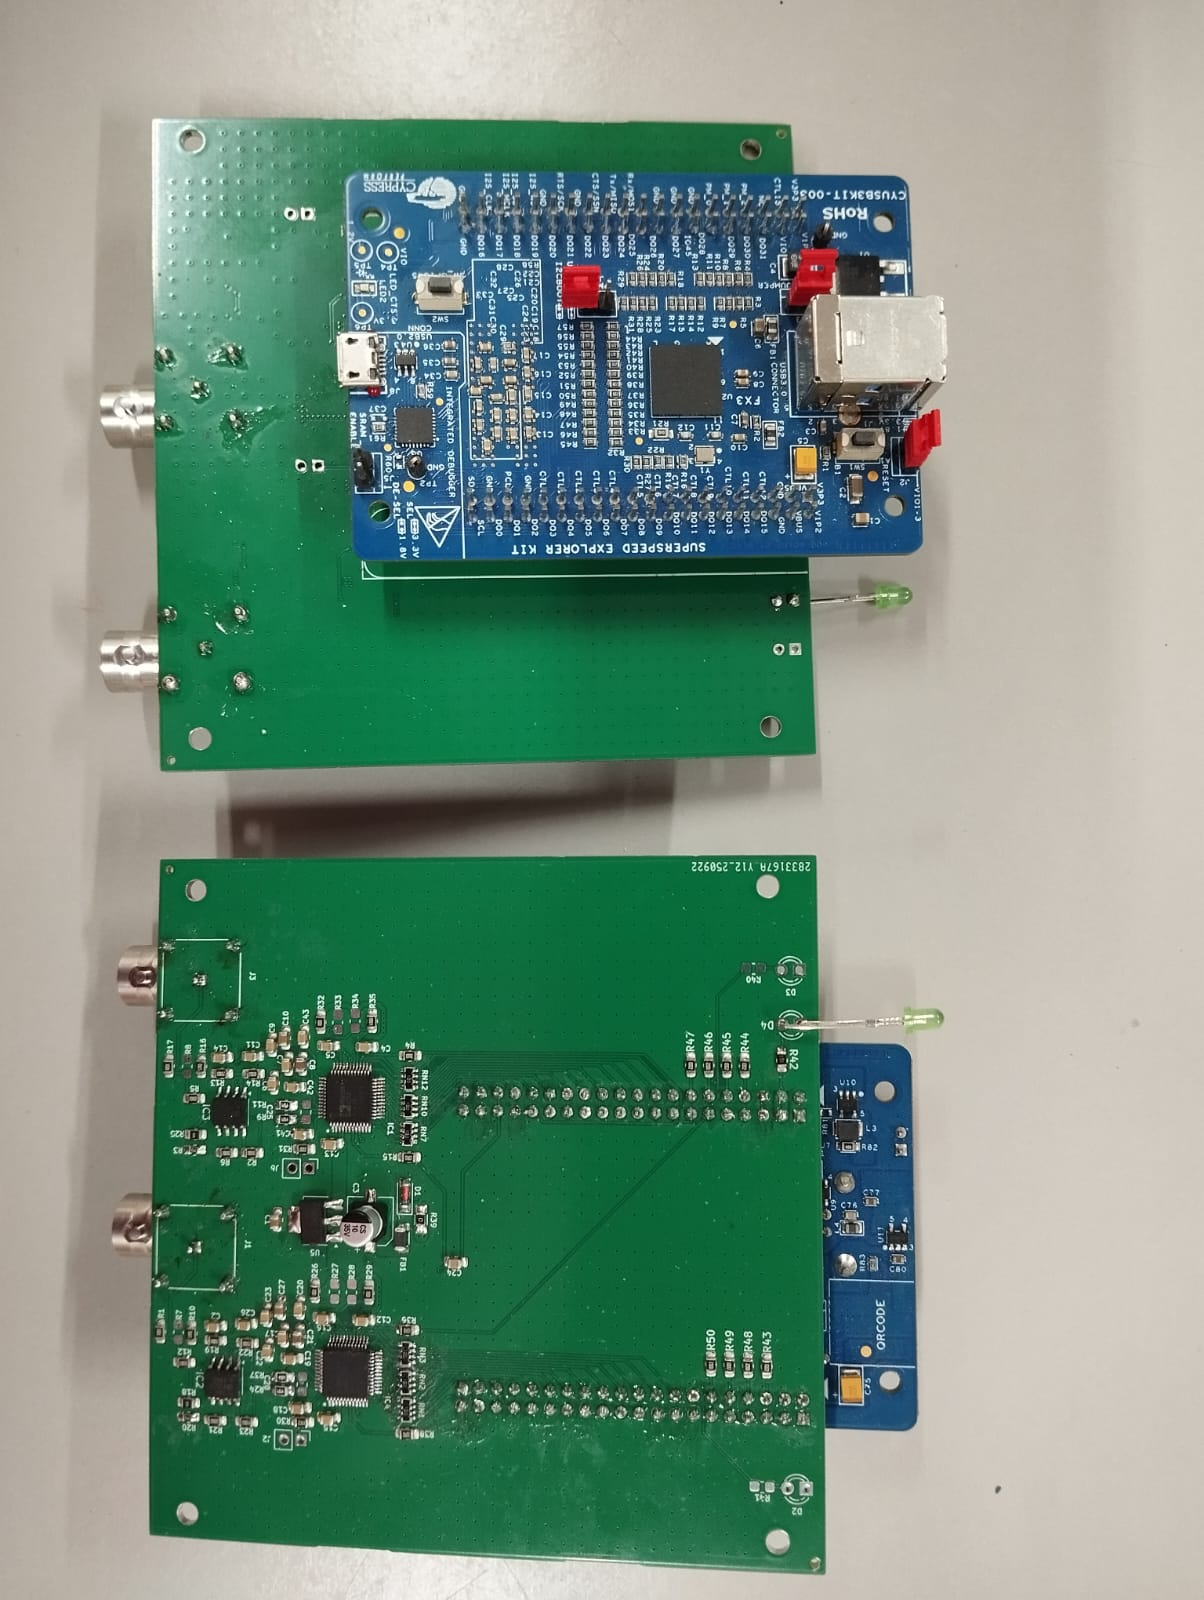
\includegraphics[angle=90, width=\linewidth]{figs/PlacasADC_AD9226.jpeg}
		\caption{Placas de captura MomeaProbe12USB.}
		\label{fig:MomeaProbe12USB}
	\end{subfigure}\hfill
	\begin{subfigure}[b]{0.58\textwidth}
		\centering
		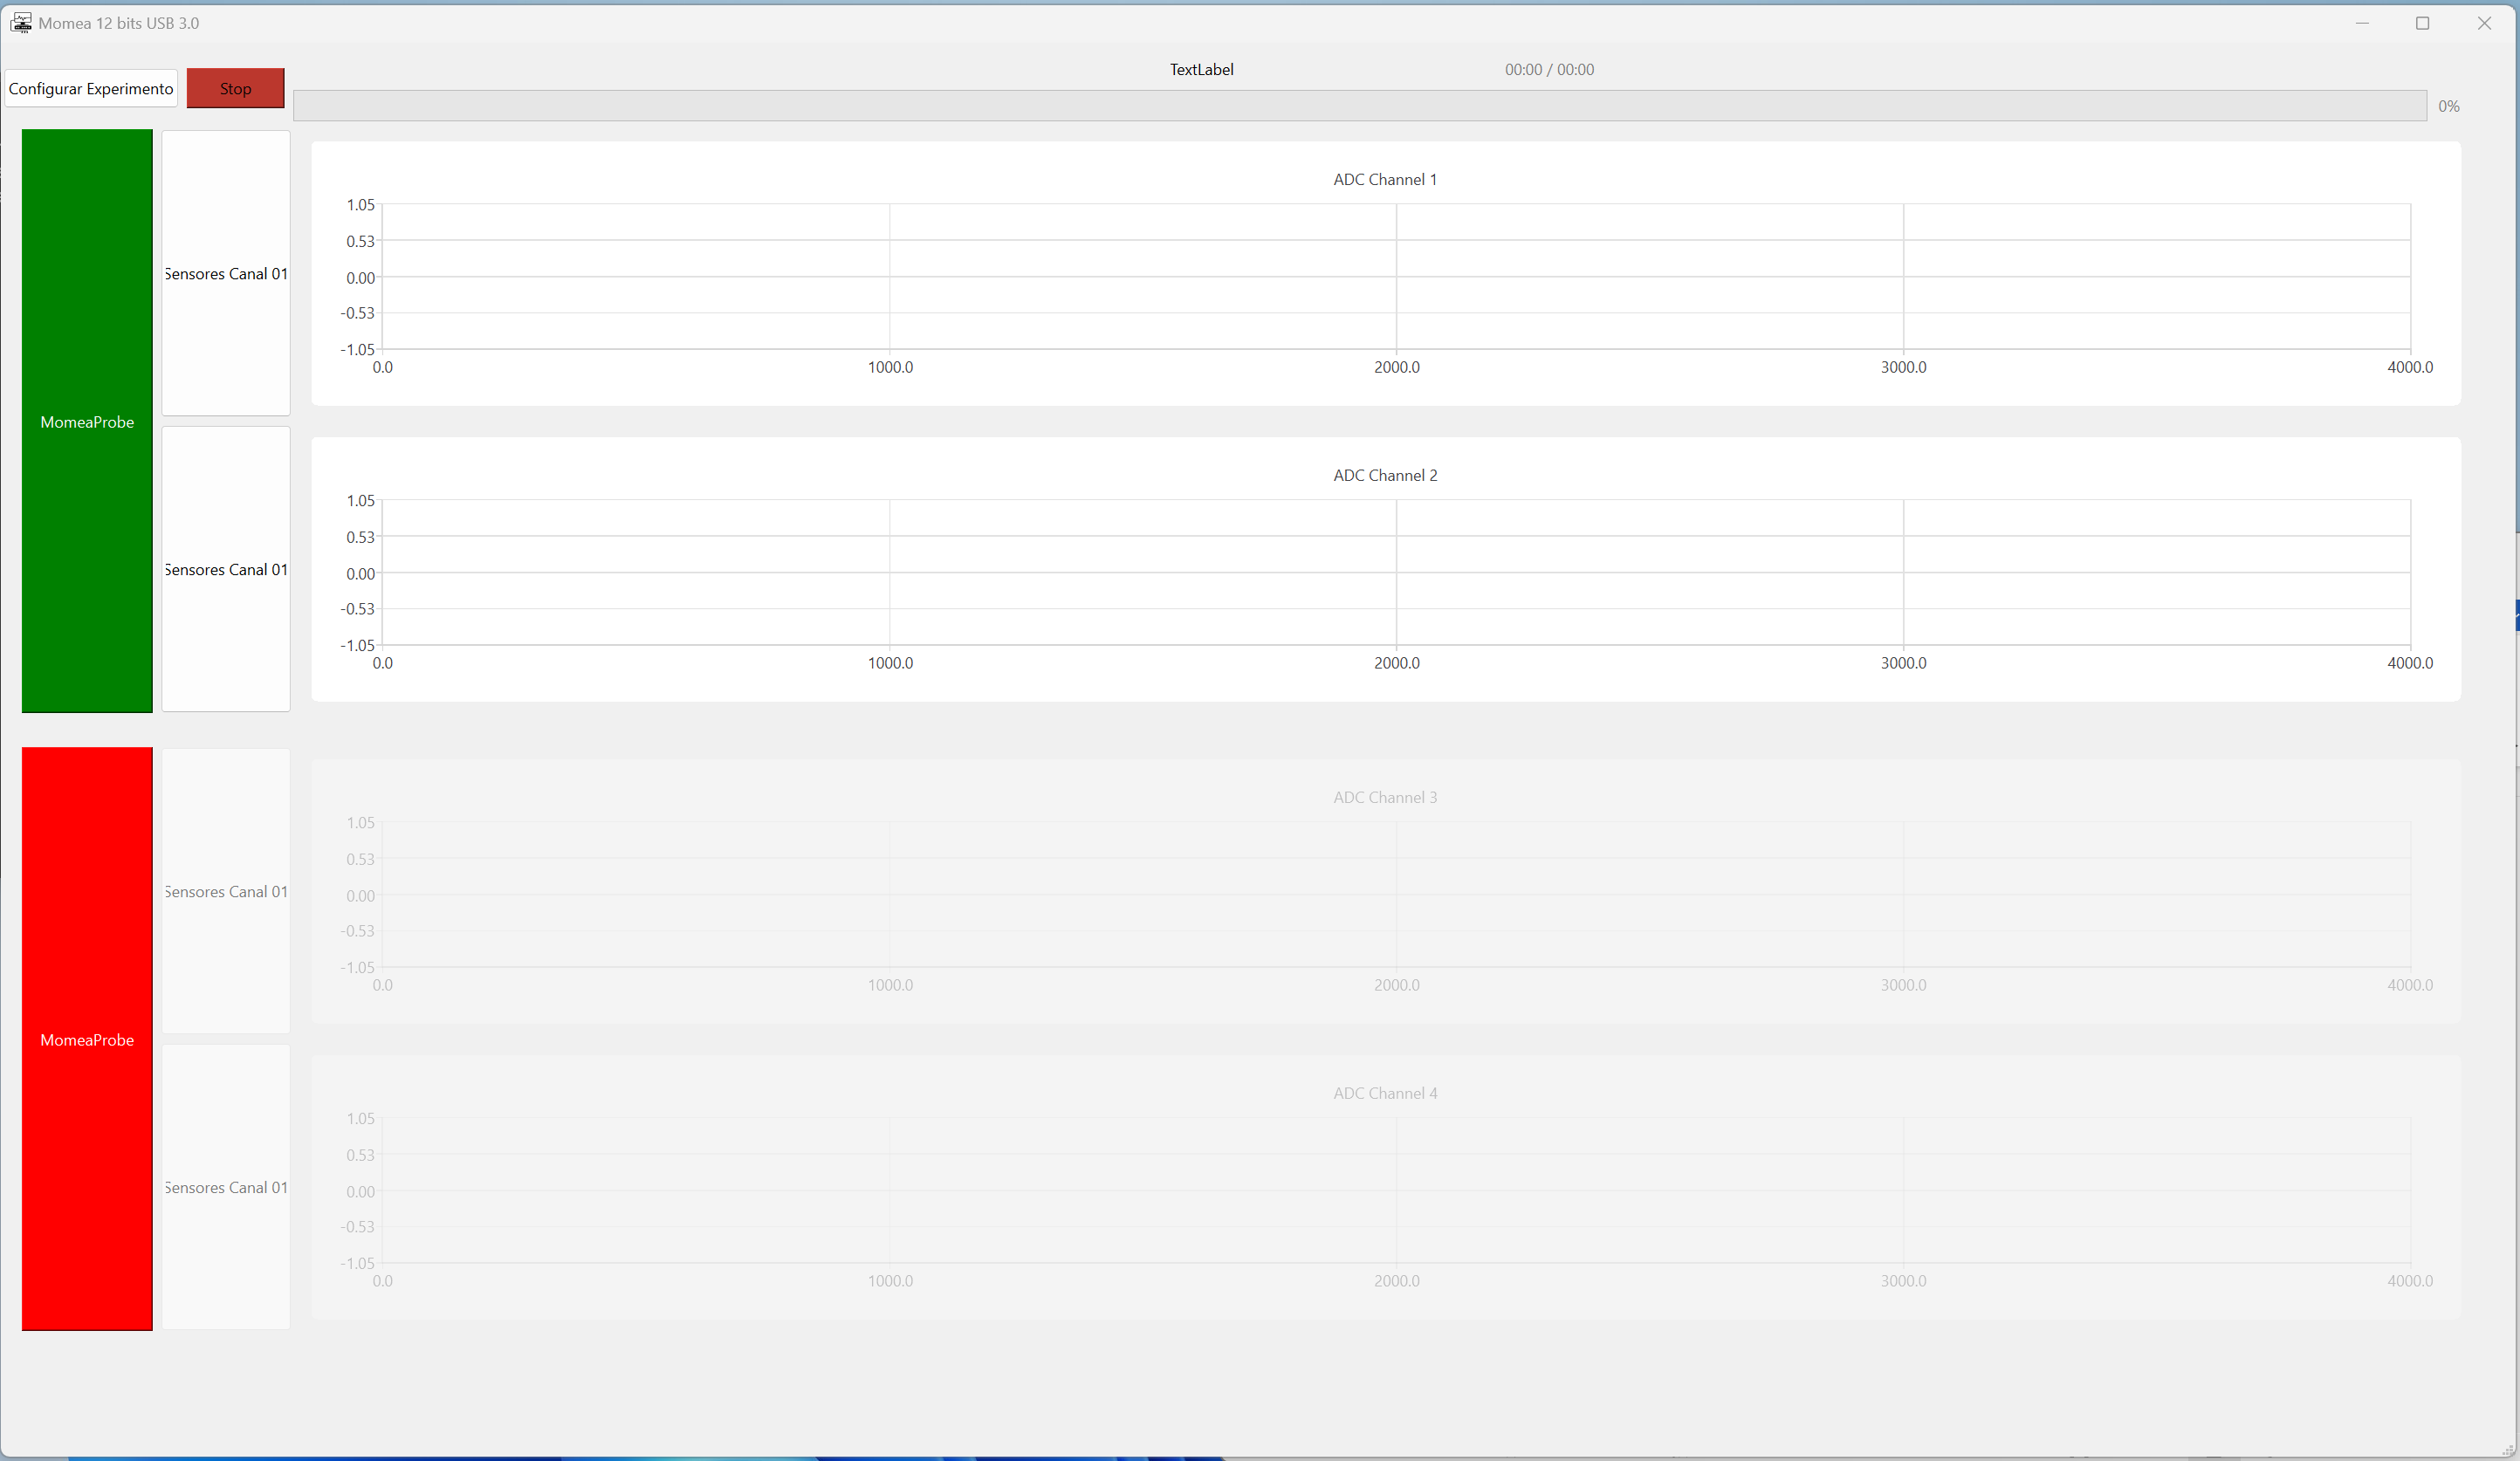
\includegraphics[width=\linewidth]{figs/MomeaCapture.png}
		\caption{Aplicação MomeaCapture.}
		\label{fig:MomeaCapture}
	\end{subfigure}
	\caption{Plataforma de aquisição contínua que antecedeu este trabalho. Fonte: o autor.}
	\label{fig:momea_usb}
\end{figure}

O uso dessa plataforma evidenciou o problema que motivou esta dissertação. A 8 a 10\,MSa/s por canal, com 12 a 16 bits por amostra, cada canal produz de 16 a 20\,MB/s, isto é, dezenas de gigabytes por hora. Manter esse fluxo exigiu, no computador, aquisição em múltiplas \textit{threads}, \textit{buffers} circulares, compactação contínua (LZMA) e escrita de alta vazão em disco. Na Figura~\ref{fig:MomeaUSB}, os dados brutos atravessam todo o caminho até a aplicação e só então são segmentados e analisados, de modo que a análise ocorre depois da gravação, e não em tempo real. A maior parte desse volume corresponde a ruído de fundo entre os eventos de interesse, que são esparsos.

\begin{figure}[htbp]
	\centering
	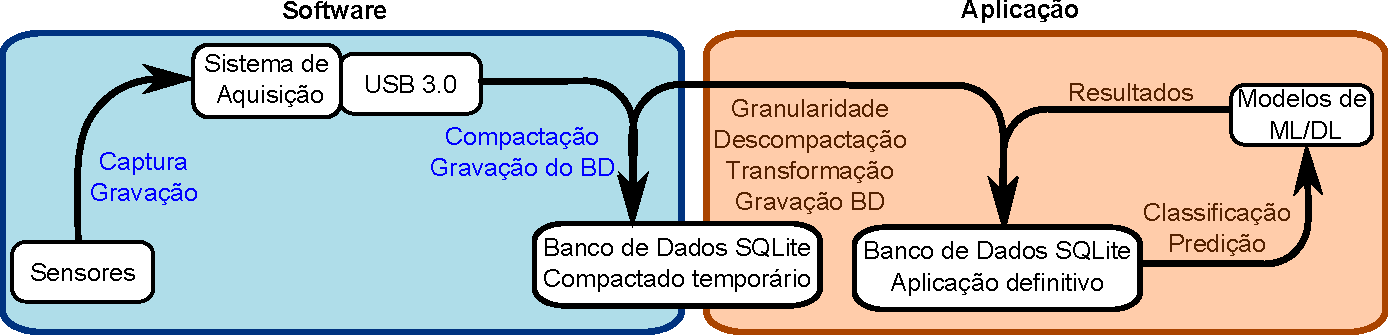
\includegraphics[width=0.95\linewidth]{figs/FluxoOperacaoMOMEAUSB}
	\caption[Fluxo de operação do sistema Momea USB]{Fluxo de operação do sistema MOMEA com aquisição contínua por USB: os dados brutos são compactados, armazenados em um banco temporário e só depois processados pela aplicação. Fonte: o autor.}
	\label{fig:MomeaUSB}
\end{figure}

A proposta desta dissertação desloca a redução de dados para antes da transmissão (Figura~\ref{fig:MomeaFPGA}): o FPGA detecta e parametriza os \textit{hits}, e apenas os registros seguem para a aplicação, por Ethernet a 100\,Mb/s. O destaque da figura é a diferença em relação ao fluxo USB: o bloco ``FPGA + HIT'' substitui a transmissão contínua de amostras, e a etapa de compactação deixa de ser necessária. As decisões que levaram a essa arquitetura são detalhadas a seguir.

\begin{figure}[htbp]
	\centering
	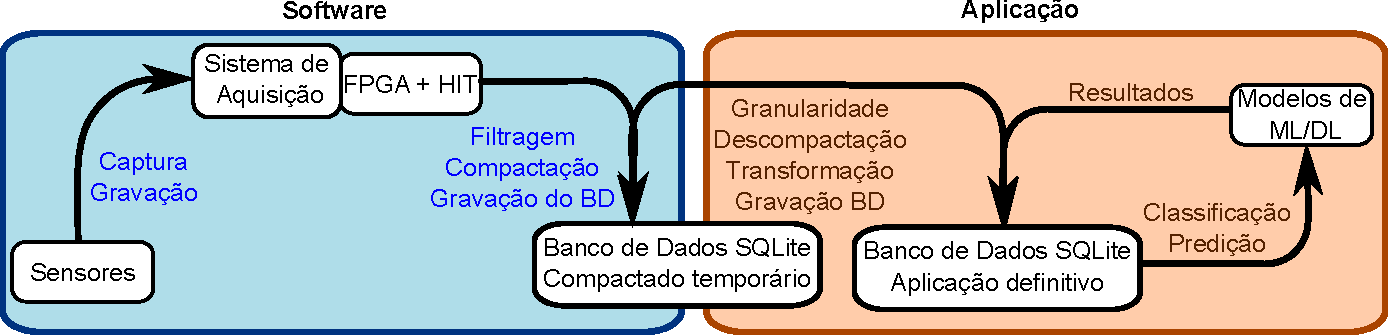
\includegraphics[width=0.9\linewidth]{figs/FluxoOperacaoMOMEAFPGA}
	\caption[Fluxo de operação do sistema Momea FPGA]{Fluxo de operação do sistema MOMEA com extração de \textit{hits} no FPGA. Em relação à Figura~\ref{fig:MomeaUSB}, o bloco ``FPGA + HIT'' (destacado) substitui a transmissão contínua das amostras. Fonte: o autor.}
	\label{fig:MomeaFPGA}
\end{figure}

% -------------------------------------------------------------------------------------------------------
\section{Arquitetura proposta: decisões de projeto}
\label{sec:mm_decisoes}
% Gerado por ferramentas/importar_relatorios.py a partir de ARTIGO_V2-10.11.2026/3-Decisoes_tecnologicas_metodologicas2.tex.
% Revisado à mão na dissertação: edite este arquivo, não a fonte.
% =======================================================================================================

Esta seção apresenta os requisitos e as decisões que conduziram à arquitetura adotada. A exposição é organizada segundo a relação requisito--alternativa--decisão--evidência, e não segundo a cronologia do desenvolvimento. O objetivo é explicitar os compromissos envolvidos e estabelecer quais resultados devem sustentar cada escolha nas Seções~\ref{sec:mm_implementacao} a~6.

% -------------------------------------------------------------------------------------------------------
\subsection{Requisitos e critérios de avaliação}
\label{v2:subsec:requisitos_arquitetura}

O cenário considerado é o monitoramento contínuo, distribuído e de longo prazo de sinais de EA. Nesse contexto, uma decisão de projeto somente pode ser considerada justificada quando o requisito correspondente é associado a um critério verificável. A Tabela~\ref{v2:tab:requisitos_sistema} resume os requisitos adotados e as evidências necessárias. Todavia, algumas informações são obtidas somente quando da realização dos ensaios, que são discutidos na Seção~\ref{sec:res_extrator}.

\begingroup
\footnotesize
\renewcommand{\arraystretch}{1.25}
\begin{longtable}{
		|>{\raggedright\arraybackslash}p{0.25\textwidth}
		|>{\raggedright\arraybackslash}p{0.34\textwidth}
		|>{\raggedright\arraybackslash}p{0.34\textwidth}|}
	\caption{Requisitos do sistema e respectivos valores quantitativos estabelecidos.}
	\label{v2:tab:requisitos_sistema}\\
	\hline
	\textbf{Requisito} & \textbf{Valor / meta} & \textbf{Situação} \\
	\hline
	\endfirsthead
	\multicolumn{3}{c}
	{\tablename\ \thetable{} -- continuação}\\
	\hline
	\textbf{Requisito} & \textbf{Valor / meta} & \textbf{Situação} \\
	\hline
	\endhead
	\hline
	\multicolumn{3}{r}{Continua na próxima página.}\\
	\endfoot
	\hline
	\endlastfoot
	Número de canais & 2 (dois canais independentes, A e B) & Definido \\
	\hline
	Taxa de amostragem efetiva & 10 MSa/s por canal ($\Delta t = 100$ ns) & Definido \\
	\hline
	Resolução do ADC & 12 bits + 1 bit de sobretensão por canal & Definido \\
	\hline
	Maior taxa sustentada de hits & Testada até 333 hits/s por canal (10\,000 \textit{bursts} em 30\,s), sem perda na comunicação (0/48\,280 registros) & Ensaio executado em 15/10/2026 (Seção~\ref{sec:res_extrator}); valor preliminar \\
	\hline
	Duração da rajada suportada & A medir (função da profundidade da FIFO/DMA) & Não ensaiada: com HLT de 2000\,\(\mu\)s cada \textit{hit} ocupa o canal por 2,27 a 2,44\,ms, e intervalos bem menores que 3\,ms exigem HLT reduzido e gerador com sequenciamento interno de rajadas \\
	\hline
	Latência admissível & A medir (caminho FSM$\to$DMA$\to$UDP$\to$receptor); mínimo de \(T_{\mathrm{HDT}} + T_{\mathrm{HLT}} = 2{,}25\,\mathrm{ms}\) após o último cruzamento & Não medida: a distribuição pedida exige instrumento com estatística de intervalos (Seção~\ref{sec:res_extrator}) \\
	\hline
	Erro máximo por descritor ($\tau_x$) & Valores iniciais propostos (Tabela~\ref{v2:tab:tau_x_iniciais}) & Metodológico; congelar antes da análise final \\
	\hline
	Custo-alvo por ponto & A consolidar (BOM do ponto completo) & A consolidar \\
\end{longtable}
\endgroup

Na versão submetida aos ensaios, o sistema tem dois canais a 10\,MSa/s e sustentou até 333 \textit{hits}/s por canal sem perda; os demais valores quantitativos são apresentados nas Seções~\ref{sec:mm_implementacao} e~\ref{sec:res_extrator}. 
% -------------------------------------------------------------------------------------------------------
\subsection{Arquitetura inicial baseada em \textit{streaming} contínuo}
\label{v2:subsec:streaming_continuo}

A plataforma inicialmente desenvolvida no Projeto MOMEA, denominada MOMEA-USB, transferia integralmente as amostras digitalizadas para um computador hospedeiro. O módulo de aquisição empregava dois conversores A/D com resolução nominal de 12 bits e taxa de amostragem de \(8\,\mathrm{MS/s}\) por canal, com transmissão por USB~3.0. A aplicação hospedeira, desenvolvida em C++ com o \textit{framework} Qt, realizava a recepção, a bufferização, o armazenamento e o processamento dos dados. 

O MOMEA-USB transporta os dois canais combinados em uma palavra de 32 bits, organizada como: 12 bits de dado + 1 bit de sobretensão + 3 bits de padding (canal A) e o mesmo arranjo para o canal B -- totalizando 16 bits por canal alinhados por byte -- e não empacotamento contínuo de 12 bits. Aplica-se compressão LZMA no nível 3 (a escala vai de 0 a 9), obtendo uma razão de compressão de aproximadamente 60\% em média (isto é, o arquivo comprimido fica em torno de 60\% do tamanho original).

A taxa associada às amostras depende do formato utilizado no transporte. Para \(N_{\mathrm{c}}\) canais, taxa \(f_{\mathrm{s}}\) e \(b_{\mathrm{tr}}\) bits transportados por amostra, a taxa sem sobrecargas é:
\begin{equation}
	R_{\mathrm{stream}} = N_{\mathrm{c}}f_{\mathrm{s}} \frac{b_{\mathrm{tr}}}{8}
	\label{v2:eq:taxa_streaming_secao3}
\end{equation}

Para dois canais a \(8\,\mathrm{MS/s}\), obtêm-se \(24\,\mathrm{MB/s}\) quando 12 bits são efetivamente empacotados e \(32\,\mathrm{MB/s}\) quando cada amostra ocupa uma palavra de 16 bits. Em aquisição ininterrupta, esses valores correspondem, respectivamente, a aproximadamente \(2{,}07\,\mathrm{TB/dia}\) e \(2{,}76\,\mathrm{TB/dia}\), antes de cabeçalhos, metadados, redundância e eventuais arquivos auxiliares.

Esses valores não mostram que o enlace USB~3.0, isoladamente, seja insuficiente. O desempenho depende da cadeia inteira, incluindo empacotamento, controlador USB, cópias em memória, escalonamento do sistema operacional, processamento, sistema de arquivos e unidade de armazenamento. A vazão sustentada medida foi de cerca de 28\,MB/s, sem perdas observadas. O sistema emprega um buffer circular de 1 GB, cuja ocupação máxima atingiu picos de cerca de 5\,\%. A aquisição durou 12 horas contínuas, a 8\,MSa/s, com compressão LZMA e sem perdas registradas pelos contadores. Assim, as limitações da arquitetura foram avaliadas por medições de vazão sustentada, ocupação dos \textit{buffers} e perdas, e não apenas pela taxa nominal da interface.

A arquitetura baseada em \textit{streaming} preserva o conjunto integral de amostras dentro dos limites de banda, resolução e ruído da cadeia. Isso mantém a possibilidade de aplicar posteriormente diferentes métodos de processamento ao mesmo registro. No cenário de operação contínua, entretanto, foram identificados três compromissos:

\begin{itemize}
	\item \textbf{Processamento e entrada/saída no computador hospedeiro:} a recepção sustentada exige bufferização, processamento concorrente e escrita com vazão suficiente. Por isso, neste trabalho, a ocorrência e a localização de perdas são demonstradas por contadores, e não inferidas de variações de desempenho.
	
	\item \textbf{Volume armazenado em relação à atividade de interesse:} em regimes esparsos, grande parte das amostras não pertence às janelas posteriormente identificadas como \textit{hits}. Essa fração depende do limiar, do DDT, da atividade observada e da definição da janela, devendo ser medida nos ensaios.
	
	\item \textbf{Latência variável:} as etapas de recepção, eventual compressão, armazenamento e análise introduzem atrasos dependentes da carga do hospedeiro e do subsistema de entrada e saída. Sem uma arquitetura de tempo real e uma análise de pior caso, não se deve atribuir limite determinístico a essa latência.
\end{itemize}

Esses compromissos não invalidam o \textit{streaming}. A preservação das formas de onda continua especialmente útil para caracterização de sinais, avaliação de novos algoritmos, investigação de 
ovo{eventos} não previstos e construção de bases de dados. A experiência com a MOMEA-USB motivou, porém, a avaliação de uma arquitetura em que o modo principal de operação transmite descritores extraídos localmente.

% -------------------------------------------------------------------------------------------------------
\subsection{Decisão pela extração de descritores na borda}
\label{v2:subsec:extracao_borda}

A arquitetura adotada desloca para o dispositivo de aquisição a detecção, a delimitação temporal e a extração dos descritores dos \textit{hits}. A decisão é adequada quando a informação requerida pelo nível superior pode ser representada por esses descritores e quando a taxa resultante é inferior à do fluxo de amostras.

Se \(\lambda_{\mathrm{h}}\) é a taxa total média de \textit{hits}, \(B_{\mathrm{reg}}\) é o tamanho do registro, \(m\) é o número médio de registros agregados por pacote, \(B_{\mathrm{ov}}\) é a sobrecarga por pacote referida ao ponto em que a vazão é avaliada e \(R_{\mathrm{aux}}\) reúne o tráfego de estado (keep-alive), comandos de configuração, mensagens de sincronização e retransmissões eventualmente implementadas, a taxa média pode ser aproximada por:
\begin{equation}
	R_{\mathrm{borda}} \approx \lambda_{\mathrm{h}}B_{\mathrm{reg}} + \frac{\lambda_{\mathrm{h}}}{m}B_{\mathrm{ov}} + R_{\mathrm{aux}}
	\label{v2:eq:taxa_borda}
\end{equation}

Todas as parcelas da Equação~\eqref{v2:eq:taxa_borda} devem ser expressas na mesma unidade, por exemplo, bytes por segundo. Para o registro de 256 bits descrito na Seção~\ref{sec:mm_implementacao}, \(B_{\mathrm{reg}}=32\) bytes, mas esse valor não inclui cabeçalhos, preenchimento, intervalo entre quadros nem retransmissões eventualmente implementadas pela aplicação. Na versão ensaiada, cada datagrama leva um único registro (\(m = 1\)), e a sobrecarga de Ethernet, IP e UDP é de 42 bytes por datagrama (46 com a sequência de verificação do quadro). A condição de redução de tráfego é
\begin{equation}
	R_{\mathrm{borda}} < R_{\mathrm{stream}}
	\label{v2:eq:condicao_reducao_borda}
\end{equation}

Desprezando a variação de \(R_{\mathrm{aux}}\) com a taxa de \textit{hits} (aproximação que deve ser verificada experimentalmente), a taxa aproximada de \textit{hits} no ponto de equilíbrio é:
\begin{equation}
	\lambda_{\mathrm{h,lim}} \approx \frac{R_{\mathrm{stream}}-R_{\mathrm{aux}}}{B_{\mathrm{reg}}+B_{\mathrm{ov}}/m}
	\label{v2:eq:taxa_limite_hits}
\end{equation}

Essa expressão evidencia que a redução não é uma constante da arquitetura. Ela depende da atividade detectada, do limiar, dos parâmetros temporais, do tamanho do registro, da agregação em pacotes e do tráfego auxiliar. A taxa de transmissão deixa de ser diretamente proporcional a \(N_{\mathrm{c}}f_{\mathrm{s}}\), mas a própria taxa de \textit{hits} ainda pode depender da amostragem, da banda e do detector.

O compromisso central é a não preservação integral da forma de onda no modo considerado. Após o descarte das amostras, não é possível recalcular os descritores com outro limiar ou outro DDT, aplicar retrospectivamente métodos baseados na forma de onda nem examinar 
ovo{eventos} não reconhecidos. A extração local é, portanto, uma transformação com perda de informação, e não uma compressão convencional com reconstrução do sinal.

Em atividade aproximadamente contínua ou sob ruído que produza muitos \textit{hits}, a vantagem de comunicação pode diminuir ou desaparecer. Além da taxa média, importa a maior rajada. Se a lógica produz registros à taxa \(\lambda_{\mathrm{in}}\), o software os retira à taxa de serviço \(\mu_{\mathrm{out}}\), e uma rajada com \(\lambda_{\mathrm{in}}>\mu_{\mathrm{out}}\) dura \(T_{\mathrm{b}}\), uma estimativa mínima para a capacidade adicional de fila é:
\begin{equation}
	C_{\mathrm{fila,min}} \geq \left(\lambda_{\mathrm{in}} - \mu_{\mathrm{out}}\right) T_{\mathrm{b}}
	\label{v2:eq:capacidade_fila_rajada}
\end{equation}

\noindent
expressa em número de registros. A validade dessa aproximação requer que as taxas sejam aproximadamente constantes durante a rajada. Quando a capacidade é excedida, o descarte é explícito e registrado por contadores de perda.

Um modo híbrido, com captura seletiva de formas de onda, pode reduzir a perda de flexibilidade analítica. Neste trabalho, esse modo não foi implementado e é tratado como extensão futura.

% -------------------------------------------------------------------------------------------------------
\subsection{Seleção da plataforma de hardware}
\label{v2:subsec:plataforma_hardware}

A seleção do hardware foi orientada pela execução contínua do caminho por amostra, pela necessidade de paralelismo nos filtros e acumuladores, pelas interfaces disponíveis, pelo custo por ponto e pela complexidade de integração. A Tabela~\ref{v2:tab:alternativas_arquitetura} resume as alternativas documentadas no desenvolvimento.

\begingroup
\footnotesize
\renewcommand{\arraystretch}{1.25}
\begin{longtable}
	{|>{\raggedright\arraybackslash}p{0.20\textwidth}
		|>{\raggedright\arraybackslash}p{0.25\textwidth}
		|>{\raggedright\arraybackslash}p{0.22\textwidth}
		|>{\raggedright\arraybackslash}p{0.20\textwidth}|}
	\caption{Alternativas arquiteturais consideradas e decisão adotada.}
	\label{v2:tab:alternativas_arquitetura}\\
	\hline
	\textbf{Alternativa} & \textbf{Vantagem preservada} & \textbf{Compromisso principal} & \textbf{Decisão} \\
	\hline
	\endfirsthead
	\multicolumn{4}{c}
	{\tablename\ \thetable{} -- continuação}\\
	\hline
	\textbf{Alternativa} & \textbf{Vantagem preservada} & \textbf{Compromisso principal} & \textbf{Decisão} \\
	\hline
	\endhead
	\hline
	\endlastfoot
	MOMEA-USB com processamento no hospedeiro & Forma de onda integral e grande flexibilidade de processamento posterior. & Vazão e armazenamento contínuos; dependência do hospedeiro; latência variável. & Linha de base. \\
	\hline
	Artix-7 com caminho de dados em lógica e MicroBlaze & Paralelismo por amostra, partição explícita entre dados e controle e ausência de processador \textit{hard} não utilizado. & O processador \textit{soft-core} e seus periféricos consomem recursos da lógica; rede e software continuam sujeitos a filas e variação temporal. & Selecionada. \\
	\hline
	Zynq-7000 com processador ARM integrado & Processador \textit{hard}, controladores e interfaces integrados ao sistema de processamento. & Complexidade de inicialização e integração entre PS e PL; eventual custo de recursos não exigidos pelo caminho crítico. & Considerada, não adotada. \\
\end{longtable}
\endgroup

O dispositivo selecionado foi o Artix-7 XC7A35T. A especificação da família informa \(33\,280\) células lógicas, \(5\,200\) \textit{slices}, 90 blocos DSP48E1 e \(1\,800\,\mathrm{Kb}\) de memória em blocos, equivalentes a 50 blocos de \(36\,\mathrm{Kb}\) \cite{xilinx2020ds180}. Como cada \textit{slice} da série 7 contém quatro LUTs e oito \textit{flip-flops}, o dispositivo oferece \(20\,800\) LUTs e \(41\,600\) registradores de \textit{slice}.

Esses números descrevem capacidade nominal, não suficiência para a aplicação. A decisão somente é sustentada pelos relatórios da versão implementada: utilização hierárquica de LUTs, registradores, BRAM e DSP; recursos de relógio e entrada/saída; potência estimada; e análise temporal pós-roteamento. O dispositivo é o Artix-7 XC7A35TICSG324-1L, encapsulamento CSG324, grau de velocidade -1L (baixa tensão, faixa industrial). A utilização e a análise temporal da versão implementada são apresentadas na Seção~\ref{sec:mm_implementacao} (Tabela~\ref{v2:tab:utilizacao_pos_implementacao}). 

A margem de recursos precisa ser avaliada em conjunto com a temporização e a largura de banda interna: baixa ocupação não garante que novos módulos possam ser acrescentados sem comprometer o fechamento temporal.

A família Zynq-7000 combina lógica programável e sistema de processamento baseado em ARM Cortex-A9 \cite{xilinx2018ds190}. No sistema proposto, o caminho por amostra é executado na lógica e as funções de controle possuem taxa inferior. Embora o Zynq pudesse oferecer maior desempenho de software, a complexidade adicional de inicialização e integração entre PS e PL não se justificava para as funções de controle requeridas, que são de baixa taxa e podem ser atendidas pelo MicroBlaze. Essa justificativa não demonstra superioridade geral do Artix-7: ela é válida para a partição adotada e deve ser complementada por comparação de custo, consumo, recursos e esforço de integração.

O argumento econômico deve considerar o ponto de medição completo. A comparação deve incluir placa de processamento, conversão A/D, condicionamento analógico, memória, comunicação, alimentação, conectores e proteções. Valores monetários devem trazer data, quantidade, moeda e natureza do item---placa de desenvolvimento, protótipo ou estimativa de produção.

% -------------------------------------------------------------------------------------------------------
\subsection{Partição entre lógica programável e software embarcado}
\label{v2:subsec:divisao_hw_sw}

A arquitetura separa o caminho de dados, executado na taxa das amostras, do caminho de controle, executado na taxa de geração e transmissão dos registros. Essa partição é resumida na Tabela~\ref{v2:tab:particao_hw_sw}.
\begin{table}[htbp]
	\centering
	\footnotesize
	\caption{Partição funcional entre lógica programável e software.}
	\label{v2:tab:particao_hw_sw}
	\renewcommand{\arraystretch}{1.25}
	\begin{tabular}
		{|>{\raggedright\arraybackslash}p{0.22\textwidth}
			|>{\raggedright\arraybackslash}p{0.35\textwidth}
			|>{\raggedright\arraybackslash}p{0.35\textwidth}|}
		\hline
		\textbf{Camada} & \textbf{Funções} & \textbf{Condição de desempenho} \\ 
		\hline
		Lógica programável & Recepção das amostras, filtragem, limiar, máquina de estados, pico, contagens e acumuladores. & Fechamento temporal; ausência de bloqueio no caminho por amostra; tratamento explícito de transbordos e cruzamentos de domínio. \\
		\hline
		MicroBlaze e FreeRTOS & Configuração, retirada e empacotamento dos registros, pilha de comunicação, comandos e informações de estado. & Tempo de serviço superior à taxa média de entrada; prioridades e filas dimensionadas para a rajada especificada. \\
		\hline
		Computador ou nível superior & Recepção, verificação de sequência, persistência, visualização e análise posterior. & Detecção de perdas, tratamento de reordenação e preservação dos metadados de configuração e sincronização. \\
		\hline
	\end{tabular}
\end{table}

A implementação em lógica explora paralelismo e produz uma latência de \textit{pipeline} expressa por número definido de ciclos, desde que todas as restrições temporais sejam satisfeitas e o caminho não seja interrompido por contenção ou contrapressão. Isso não torna fixa a latência de emissão do registro: o registro somente pode ser consolidado depois do último cruzamento e da expiração do DDT.

O MicroBlaze executa FreeRTOS para organizar tarefas assíncronas de comunicação e configuração. O escalonamento preemptivo facilita a atribuição de prioridades, mas não garante, isoladamente, ausência de perda ou prazo de resposta. Da arquitetura tem-se: processador soft-core MicroBlaze executando FreeRTOS e pilha lwIP, com transferência dos registros por DMA e transmissão UDP. Quando da pós-implementação será discutida a frequência do processador, as prioridades das tarefas, os tempos máximos de execução, as interrupções, a profundidade das filas, a política de \textit{cache} e o mecanismo de coerência com o DMA, quando aplicável.

Se a latência for medida desde a entrada da amostra correspondente ao primeiro cruzamento até a disponibilização do registro no receptor, uma decomposição apropriada é \(L_{\mathrm{total}} = L_{\mathrm{pipe}} + t_{\mathrm{dur}} + T_{\mathrm{DDT,impl}} + L_{\mathrm{fin}} + L_{\mathrm{fila}} + L_{\mathrm{SW}} + L_{\mathrm{rede}}\), em que \(L_{\mathrm{pipe}}\) é a latência até a decisão correspondente, \(t_{\mathrm{dur}}\) é a duração entre primeiro e último cruzamentos, \(L_{\mathrm{fin}}\) é a finalização do registro na lógica e as três últimas parcelas representam fila, software e rede. Se a referência temporal for o último cruzamento, o termo \(t_{\mathrm{dur}}\) deve ser omitido. Apenas \(L_{\mathrm{pipe}}\), \(T_{\mathrm{DDT,impl}}\) e \(L_{\mathrm{fin}}\) podem ser associados diretamente a quantidades determinadas de ciclos; as demais parcelas dependem da carga.

% -------------------------------------------------------------------------------------------------------
\subsection{Comunicação, observabilidade de perdas e sincronização}
\label{v2:subsec:interface_comunicacao}

Adotou-se Ethernet 10/100 para desacoplar o ponto de aquisição de uma conexão USB direta e permitir sua integração a uma rede comutada. No modo de \(100\,\mathrm{Mb/s}\), a taxa nominal do enlace equivale a \(12{,}5\,\mathrm{MB/s}\); no modo de \(10\,\mathrm{Mb/s}\), equivale a \(1{,}25\,\mathrm{MB/s}\). A vazão útil é menor devido aos cabeçalhos, ao preenchimento, ao preâmbulo e ao intervalo entre quadros. Nos ensaios, o enlace operou no modo de 100\,Mb/s. 

Para taxa de pacotes \(\lambda_{\mathrm{p}}\), conteúdo útil médio \(B_{\mathrm{payload}}\) e sobrecarga por pacote \(B_{\mathrm{ov,rede}}\), a taxa no enlace pode ser estimada por 
\begin{equation}
	R_{\mathrm{rede}} \approx 8\lambda_{\mathrm{p}} \left(B_{\mathrm{payload}} + B_{\mathrm{ov,rede}}\right)
	\label{v2:eq:taxa_rede}
\end{equation}

\noindent
em bits por segundo. A definição de \(B_{\mathrm{ov,rede}}\) deve indicar se a medição considera apenas UDP/IP, o quadro Ethernet ou todos os elementos transmitidos no meio físico.

Os registros são transportados por UDP. Esse protocolo reduz o estado e os mecanismos do transporte, mas não garante entrega, ordenação nem proteção contra duplicação \cite{postel1980udp}. A decisão por UDP deve, portanto, ser acompanhada na camada de aplicação por número sequencial de pacotes, quantidade de registros por pacote, contador cumulativo de registros produzidos e indicação de reinicialização. 

O cabeçalho de aplicação com versão do protocolo, identificação do dispositivo, número de sequência, quantidade de registros, contador cumulativo, carimbo de tempo de referência, tamanho do conteúdo e indicadores de erro ou reinicialização foi especificado, mas não implementado na versão ensaiada. Cada datagrama da porta 5007 leva apenas os 32 bytes de um registro de \textit{hit}, sem cabeçalho de aplicação nem número de sequência gerado no dispositivo. Na versão ensaiada, a observabilidade de perdas é obtida por contadores independentes em cada etapa: na lógica, o contador \texttt{HITCNT} (\textit{hits}, ROVL e MAXDUR por canal) e os registradores de depuração do mapa AXI; no firmware, os contadores de transferências do DMA e de falhas de envio; e, no receptor, a numeração dos datagramas e dos registros na chegada. Ao fim de cada captura, o \textit{software} de aquisição compara o total de registros contado na lógica com o total recebido e gravado, de modo que \(N_{\mathrm{perdidos}} = N_{\mathrm{HITCNT}} - N_{\mathrm{rx}}\). Duplicações e trocas de ordem não são detectáveis individualmente sem número de sequência; o risco é reduzido pelo enlace direto entre a placa e o computador, sem comutadores. O cabeçalho especificado permanece como evolução prevista, e o campo de 32 bits livre no registro é candidato a número de sequência.

A Ethernet também não fornece determinismo temporal nem qualificação industrial por si só. A robustez física depende de transceptor, isolamento, conectores, cabeamento, alimentação, proteção contra transientes e compatibilidade eletromagnética. A latência depende das filas, da pilha, do controlador, dos comutadores e da carga da rede.

Se registros de diferentes canais ou dispositivos forem correlacionados pelo tempo, deve existir mecanismo explícito de sincronização. A arquitetura prevista é um carimbo de tempo gerado por um contador livre no FPGA, com largura de 64 bits e resolução de 100 ns (um período de amostra a 10 MHz, igual à grade do AMSY-6), com época zerada nos comandos START e STOP. O campo correspondente já está reservado no registro do \textit{hit}, mas o \textit{bitstream} ensaiado o envia zerado. Como a conectividade Ethernet não estabelece base de tempo comum, a sincronização com o AMSY-6 prevista é um sinal de disparo do gerador aplicado às duas cadeias, com associação entre estímulos e \textit{hits} por janelas temporais em torno de cada disparo. Sem o carimbo, essa associação \textit{hit} a \textit{hit} e a medição da deriva entre as bases de tempo não são possíveis; nos ensaios desta etapa, a associação foi feita por bloco de estímulos.

% -------------------------------------------------------------------------------------------------------
\subsection{Verificação instrumental e validação no domínio de aplicação}
\label{v2:subsec:metodologia_validacao}

O trabalho distingue \textit{verificação instrumental} e \textit{validação no domínio de aplicação}. A primeira examina se a cadeia elétrica e digital implementa os descritores especificados. A segunda examina se o instrumento fornece informação útil para detectar ou caracterizar cavitação no ambiente de uso. As duas etapas respondem a perguntas diferentes e não são equivalentes.

\subsubsection{Estratégias experimentais}
Duas estratégias são complementares:

\begin{description}
	\item[Estímulo elétrico controlado:] um gerador produz formas de onda com amplitude, duração, frequência, fase e espaçamento configurados. A injeção após o sensor elimina da avaliação os efeitos do acoplamento e da propagação mecânica e é adequada para verificar aquisição, detecção e parametrização.
	
	\item[Ensaio de cavitação:] inclui o fenômeno físico, o sensor, o acoplamento, a estrutura e o ruído da máquina. É necessário para a validação no domínio, mas não isola com facilidade erros da eletrônica ou do algoritmo, pois as fontes físicas ativas não são diretamente conhecidas.
\end{description}

Este trabalho adota, nesta etapa, o estímulo elétrico controlado. Logo, suas conclusões limitam-se à parte da cadeia posterior ao ponto de injeção. O ensaio não valida sensor, acoplamento, propagação estrutural nem capacidade de discriminar cavitação em operação real.

\subsubsection{Hierarquia das referências}
Os valores configurados no gerador não constituem referência exata. Cabos, divisores, terminações, impedâncias de entrada e largura de banda modificam o sinal. A metodologia deve distinguir quatro níveis:

\begin{enumerate}
	\item Os valores nominais programados no gerador;
	
	\item A forma de onda efetivamente aplicada em um plano de referência elétrico, medida por instrumento independente com calibração, largura de banda, taxa de amostragem e incerteza conhecidas;
	
	\item Os descritores de referência calculados \textit{off-line} a partir dessa forma de onda, empregando as definições da Seção~\ref{sec:fund_hits} e convenções explícitas de amostragem, limiar e janela; e
	
	\item Os descritores do AMSY-6, utilizado como instrumento de comparação, mas não como 
ovo{referência primária}.
\end{enumerate}

A mesma forma de onda é aplicada simultaneamente às duas cadeias, por meio de um divisor cujas atenuação, largura de banda, isolamento e impedâncias precisam ser caracterizados; em ensaios sequenciais, a repetibilidade e a deriva do gerador entram na avaliação de incerteza. Os instrumentos são um gerador de sinais e um osciloscópio digital Minipa MVB DSO de 100\,MHz, usado como referência da forma de onda (nível 2 da hierarquia de referências), com as características da Tabela~\ref{v2:tab:instrumentos}.

\begingroup
\footnotesize
\renewcommand{\arraystretch}{1.25}
\begin{longtable}{
		|>{\raggedright\arraybackslash}p{0.19\textwidth}
		|>{\raggedright\arraybackslash}p{0.34\textwidth}
		|>{\raggedright\arraybackslash}p{0.38\textwidth}|}
	\caption{Instrumentos utilizados nos ensaios e respectivas especificações principais.}
	\label{v2:tab:instrumentos}\\
	\hline
	\textbf{Instrumento} & \textbf{Especificação} & \textbf{Valor / Observação} \\
	\hline
	\endfirsthead
	\multicolumn{3}{c}
	{\tablename\ \thetable{} -- continuação}\\
	\hline
	\textbf{Instrumento} & \textbf{Especificação} & \textbf{Valor / Observação} \\
	\hline
	\endhead
	\hline
	\multicolumn{3}{r}{Continua na próxima página.}\\
	\endfoot
	\hline
	\endlastfoot
	Osciloscópio digital & Modelo & Minipa, linha MVB DSO, 100 MHz \\
	\hline
	& Banda (upgrade) & 50 / 70 / 100 MHz \\
	\hline
	& Amostragem em tempo real & até 1 GSa/s \\
	\hline
	& Amostragem acumulativa & 50 GSa/s por canal (sinais repetitivos) \\
	\hline
	& Canais de entrada & 2 \\
	\hline
	& Base de tempo & 2 ns ~ 50 s/DIV \\
	\hline
	& Fator de deflexão vertical & 1 mV ~ 20 V/DIV \\
	\hline
	& Precisão vertical básica & 3\% \\
	\hline
	& Precisão horizontal básica & ±50 ppm \\
	\hline
	& Tempo de subida & 3,5 ns \\
	\hline
	& Tensão máxima de entrada & 400 V (DC + pico AC), 1 MHz \\
	\hline
	& Memória por canal & 25 kByte \\
	\hline
	Gerador de sinais & Modelo & Rigol DG832, 2 canais, 35 MHz \\
	\hline
	& Canais & 2 \\
	\hline
	& Frequência (seno) & 1 µHz ~ 35 MHz \\
	\hline
	& Taxa de amostragem & até 125 MSa/s \\
	\hline
	& Resolução vertical & 16 bits \\
	\hline
	& Profundidade de memória & 2 Mpts padrão (8 Mpts opcional) \\
	\hline
	& Estabilidade de frequência & ±1 ppm \\
	\hline
	& Ruído de fase & -105 dBc/Hz \\
	\hline
	& Jitter de saída & tão baixo quanto 200 ps \\
	\hline
	& Precisão de frequência & ±(1 ppm do ajuste + 10 µHz), 18--28 °C \\
	\hline
	& Formas de onda arbitrárias & até 160 integradas; edição por PC \\
	\hline
\end{longtable}
\endgroup

\subsubsection{Matriz de ensaios e critérios de aceitação}
A matriz de ensaios deve explorar não apenas condições nominais, mas também fronteiras que revelem diferenças de implementação:

\begin{itemize}
	\item Amplitudes próximas ao limiar e próximas à saturação;
	
	\item Diferentes frequências dentro da banda e próximas às frequências de corte;
	
	\item Durações e números de ciclos distintos; 
	
	\item Separações de \(N_{\mathrm{DDT}}-1\), \(N_{\mathrm{DDT}}\) e \(N_{\mathrm{DDT}}+1\) amostras;
	
	\item Condições comparáveis nas proximidades do RAT, quando houver comparação de cascatas; e
	
	\item Repetições suficientes para estimar dispersão, perdas e repetibilidade.
\end{itemize}

Para cada descritor \(x\), podem ser calculados o erro \(e_x = x_{\mathrm{prop}} - x_{\mathrm{ref}}\), e, quando \(x_{\mathrm{ref}}\) estiver suficientemente afastado de zero, o erro relativo
\begin{equation}
	e_{x,\mathrm{rel}} = \frac{x_{\mathrm{prop}}-x_{\mathrm{ref}}}{x_{\mathrm{ref}}}
	\label{v2:eq:erro_relativo_descritor}
\end{equation}

O erro relativo não é usado para referências nulas ou muito pequenas; nesses casos, usa-se o erro absoluto ou o desvio em unidades de resolução (LSB ou equivalente). Em ensaios repetidos, reportam-se viés, dispersão e intervalos de incerteza, além das taxas de detecção, perda e fragmentação. A avaliação de incerteza considera gerador, instrumento independente, divisor, ganho, resolução temporal, quantização e repetibilidade, seguindo princípios compatíveis com o JCGM~100 \cite{jcgm2008}.

Os limites de aceitação devem ser definidos antes da interpretação dos resultados e relacionados à resolução e à incerteza de cada descritor. Os valores iniciais de \(\tau_x\) da Tabela~\ref{v2:tab:tau_x_iniciais} partem da resolução de cada descritor e das componentes de incerteza descritas na Seção~\ref{sec:mm_delineamento}. A base do AMSY-6 provém da especificação do fabricante, e a do sistema proposto, dos componentes da cadeia. A banda do osciloscópio de referência (100 MHz) é adequada, mas sua precisão vertical de 3\,\% é a maior componente de incerteza da referência de amplitude e, como a energia é proporcional ao quadrado da tensão, da referência de energia, cuja incerteza relativa é \(2 \times 3\,\% \approx 6\,\%\). A referência de tempo do osciloscópio (\(\pm 50\) ppm) é folgada para os descritores temporais. A coluna de repetibilidade traz o desvio-padrão medido no ensaio simultâneo de 15/10/2026 como dado de entrada, e não como critério escolhido a partir do resultado.

\begingroup
\footnotesize
\renewcommand{\arraystretch}{1.25}
\begin{longtable}{
		|>{\raggedright\arraybackslash}p{0.11\textwidth}
		|>{\raggedright\arraybackslash}p{0.21\textwidth}
		|>{\raggedright\arraybackslash}p{0.15\textwidth}
		|>{\raggedright\arraybackslash}p{0.17\textwidth}
		|>{\raggedright\arraybackslash}p{0.22\textwidth}|}
	\caption{Valores iniciais propostos para as tolerâncias \(\tau_x\).}
	\label{v2:tab:tau_x_iniciais}\\
	\hline
	\textbf{Descritor} & \textbf{Base no sistema proposto (componentes)} & \textbf{Base no AMSY-6 (fabricante)} & \textbf{Repetibilidade medida no sistema proposto (15/10)} & \textbf{\(\tau_x\) inicial proposto} \\
	\hline
	\endfirsthead
	\hline
	\textbf{Descritor} & \textbf{Base no sistema proposto} & \textbf{Base no AMSY-6} & \textbf{Repetibilidade} & \textbf{\(\tau_x\) inicial} \\
	\hline
	\endhead
	\hline
	\endlastfoot
	Amplitude & 1 LSB referido à entrada (3,13--3,23\,mV no ADC) + incerteza do ganho do pré-amplificador (34,00\,dB medidos) & Não informada na especificação consultada & \(\sigma = 0{,}04\)--\(0{,}06\)\,dB & \(\pm\)(1 LSB + \(u\) do ganho); contra a referência do osciloscópio, \(\pm 3\,\%\) (\(0{,}26\)\,dB) \\
	\hline
	Tempo de subida & 1 amostra (100\,ns) + fase do \textit{burst} em relação à grade de 10\,MHz & Resolução de 100\,ns (ASIP-2 a 10\,MHz) & Não aplicável com envelope retangular (pico ambíguo) & \(\pm 1\) amostra + \textit{jitter} de fase; avaliado só com envelope realista \\
	\hline
	Duração & 1--2 amostras (100--200\,ns) + convenção de término & 100\,ns & \(\sigma = 0{,}04\)--\(0{,}06\,\mu\)s & \(\pm 2\) amostras; comparação com o AMSY-6 apenas como descritor assemelhado \\
	\hline
	Contagens & Discreto; depende do limiar e do sinal de decisão & Discreto & Constante (10) em 48\,197 de 48\,198 \textit{hits} & \(\pm 1\) \\
	\hline
	Energia & \(2\times\) a incerteza relativa da amplitude (entra ao quadrado) & Definição de eu do fabricante & 0,12--0,64\,\% (desvio relativo) & \(\pm 6\,\%\) contra a referência; comparação com o AMSY-6 apenas como descritor assemelhado \\
\end{longtable}
\endgroup

 Uma forma geral é:
\begin{equation}
	\left|x_{\mathrm{prop}} - x_{\mathrm{ref}} \right| \leq \tau_x
	\label{v2:eq:criterio_aceitacao_descritor}
\end{equation}

\noindent
em que \(\tau_x\) é a tolerância previamente estabelecida. A comparação com o AMSY-6 avalia concordância entre implementações; a comparação com os descritores derivados da forma de onda medida fornece referência independente. Nenhuma das duas substitui a posterior validação em uma bancada de cavitação.
% =======================================================================================================


% -------------------------------------------------------------------------------------------------------
\section{Implementação do extrator de \textit{hits}}
\label{sec:mm_implementacao}
% Gerado por ferramentas/importar_relatorios.py a partir de ARTIGO_V2-10.11.2026/4-Implementacao_sistema2.tex.
% Revisado à mão na dissertação: edite este arquivo, não a fonte.
% =======================================================================================================

Esta seção descreve a implementação da cadeia de aquisição, detecção, parametrização e transmissão dos registros de \textit{hits}. O protótipo avaliado nos ensaios da Seção~\ref{sec:res_extrator} foi construído segundo a arquitetura descrita a seguir. A exposição distingue os elementos confirmados no protótipo das informações que ainda dependem de verificação final no esquemático, no código-fonte e nos relatórios das ferramentas de desenvolvimento.

% -------------------------------------------------------------------------------------------------------
\subsection{Visão geral da arquitetura}
\label{v2:subsec:visao_geral_arquitetura}

O sistema adota uma organização funcional comparável à encontrada em instrumentos de EA, sem pretender reproduzir integralmente a arquitetura interna de um equipamento comercial. A cadeia compreende sensor, pré-amplificação, filtragem e ganho analógicos, conversão A/D, processamento em lógica programável, software embarcado e comunicação Ethernet.

\begin{figure}[htbp]
	\centering
	\IfFileExists{figuras/arquitetura_geral_sistema.pdf}
	{
		\includegraphics[width=\textwidth]
		{figuras/arquitetura_geral_sistema.pdf}
	}
	{
		\fbox{
			\parbox[c][4.0cm][c]{0.92\textwidth}{
				\centering
				\textbf{Diagrama da arquitetura}\\[0.3cm] (arquivo \texttt{figuras/arquitetura\_geral\_sistema.pdf})
				
			}
		}
	}
	\caption{Arquitetura geral do sistema embarcado de aquisição, detecção e parametrização de \textit{hits} de emissão acústica.}
	\label{v2:fig:arquitetura_geral}
\end{figure}

No domínio analógico, o sinal proveniente do sensor é amplificado e limitado em banda antes de ser adequado à faixa de entrada do conversor. O filtro analógico participa da rejeição das componentes que poderiam sofrer \textit{aliasing}; essa função não pode ser transferida integralmente para o processamento digital, pois componentes já sobrepostas à banda útil após a amostragem não podem ser separadas posteriormente.

No domínio digital, a lógica programável recebe as amostras, executa a filtragem, compara o sinal processado com o limiar, delimita os \textit{hits} e acumula seus descritores. Os registros consolidados são encaminhados ao subsistema com MicroBlaze e FreeRTOS, que realiza a retirada, o empacotamento, o atendimento aos comandos de configuração e a transmissão por UDP.

As interfaces da versão ensaiada, com largura, taxa, relógio e controle de fluxo, são:
\begin{itemize}
	\item ADC AD9226 \(\rightarrow\) \texttt{adc12\_frontend}: 2 canais \(\times\) 12 bits + OTR, 10\,MSa/s, relógio de 10\,MHz gerado por MMCM;
	\item filtro IIR (\texttt{adc\_ctrl\_axi} / \texttt{iir\_biquad\_df2}): Butterworth passa-baixas de 4ª ordem (2 \textit{biquads}), coeficientes Q3.17 de 20 bits, domínio de 100\,MHz;
	\item extrator (\texttt{ae\_hit\_extractor} rev 0.08, dentro do \texttt{ae\_hit\_axi\_wrapper} rev 0.08) \(\rightarrow\) \texttt{hit\_to\_axis} rev 0.07: palavra de 256 bits, AXI-Stream com TLAST ao fim de cada \textit{hit};
	\item \texttt{axis\_data\_fifo} \(\rightarrow\) AXI DMA (S2MM, modo simples) \(\rightarrow\) DDR3 pelo controlador MIG (interface a 81,25\,MHz; referência de 200\,MHz);
	\item MicroBlaze + FreeRTOS + lwIP (100\,MHz) \(\rightarrow\) AXI Ethernet Lite (PHY a 25\,MHz) \(\rightarrow\) UDP: comandos na porta 5006 e registros na porta 5007;
	\item controle de fluxo: sinal \texttt{tready} do AXI-Stream; estouro da FIFO sinalizado por \texttt{overflow\_out} do \texttt{hit\_to\_axis}.
\end{itemize}

% -------------------------------------------------------------------------------------------------------
\subsection{\textit{Front-end} analógico}
\label{v2:subsec:front_end_analogico}

O \textit{front-end} analógico realiza o acoplamento elétrico com o sensor, a amplificação, a limitação de banda e a adequação do sinal à entrada do conversor A/D. São utilizados dois sensores Vallen: o VS45-H (sensor de baixa frequência, faixa nominal 30–100 kHz) e o VS900-M (sensor de banda larga).

Em primeira aproximação e fora das regiões de ressonância, um sensor piezoelétrico pode ser representado por uma fonte de tensão associada a uma capacitância \(C_{\mathrm{s}}\). Sua impedância é, portanto, dependente da frequência:
\begin{equation}
	Z_{\mathrm{s}}(f)
	\approx
	\frac{1}{j2\pi f C_{\mathrm{s}}},
	\label{v2:eq:impedancia_sensor}
\end{equation}
sendo utilizado apenas para ilustrar a dependência frequencial da impedância, e não como substituto da resposta eletromecânica completa do transdutor.

O pré-amplificador utilizado nos ensaios possui ganho de patamar medido de \(34{,}00\,\mathrm{dB}\), próximo do ganho nominal do pré-amplificador AEP5 usado com o AMSY-6 (34\,dB). A descrição anterior deste texto (três amplificadores AD8065, com \textit{buffer} seguido de dois estágios de ganho 10, totalizando 40\,dB nominais) não corresponde ao circuito efetivamente ensaiado.

Ganho e banda foram medidos por varredura de 1\,kHz a 35\,MHz, com 100\,mVpp injetados pelo gerador e saída lida no osciloscópio de referência, na mesma montagem de cabos RG59 e divisor usada nos ensaios. Os resultados estão na Tabela~\ref{v2:tab:preamp_medido}. A versão original do circuito tinha corte superior em \(\approx 0{,}99\,\mathrm{MHz}\), abaixo da meta de 2\,MHz; a modificação do circuito levou o corte para \(\approx 2{,}5\,\mathrm{MHz}\), sem saturação na faixa. Também foi eliminada a oscilação de 43\,MHz que surgia no \textit{buffer} de entrada com o cabo do sensor conectado: o resistor de isolação na entrada passou de \(100\,\Omega\) para \(1\,\mathrm{k}\Omega\).

\begin{table}[htbp]
	\centering
	\footnotesize
		\caption{Ganho e banda medidos dos pré-amplificadores.}
	\label{v2:tab:preamp_medido}
	\begin{tabular}{|p{0.30\textwidth}|p{0.14\textwidth}|p{0.16\textwidth}|p{0.26\textwidth}|}
		\hline
		\textbf{Pré-amplificador} & \textbf{Ganho de patamar} & \textbf{Corte superior (\(-3\,\mathrm{dB}\))} & \textbf{Observação} \\
		\hline
		Sistema proposto, versão original & 33,90\,dB & \(\approx 0{,}99\,\mathrm{MHz}\) & Abaixo da meta de 2\,MHz \\
		\hline
		Sistema proposto, após modificação (usado nos ensaios) & 34,00\,dB & \(\approx 2{,}50\,\mathrm{MHz}\) & Atende a meta de 2\,MHz; sem saturação na faixa \\
		\hline
		Vallen AEP5 (referência) & 34,22\,dB & \(\approx 4{,}10\,\mathrm{MHz}\) & Próximo do nominal de 34\,dB \\
		\hline
	\end{tabular}
\end{table}

Todas as conversões entre \(\mathrm{dB}_{\mathrm{AE}}\) e códigos do ADC usam o ganho de 34\,dB: por exemplo, o limiar de \(80\,\mathrm{dB}_{\mathrm{AE}}\) corresponde a 155 códigos, ou \(\approx 0{,}50\,\mathrm{V}\) na entrada da placa.

O AD8065 é um amplificador de realimentação de tensão com entrada FET. A documentação informa, entre outros valores típicos, corrente de polarização de entrada de \(1\,\mathrm{pA}\), densidade espectral de ruído de tensão de \(7\,\mathrm{nV}/\sqrt{\mathrm{Hz}}\) a \(10\,\mathrm{kHz}\) e largura de banda de \(145\,\mathrm{MHz}\) em ganho unitário \cite{analogdevicesad8065}. Esses números não demonstram, isoladamente, a adequação do circuito montado. A banda do conjunto e a estabilidade com o cabo do sensor foram tratadas acima.

Denotando por \(G_{\mathrm{pre}}(f)\) a resposta do pré-amplificador, por \(H_{\mathrm{PB}}(f)\) a resposta do filtro passa-banda analógico e por \(G_{\mathrm{aj}}(f)\) a resposta do estágio de ganho ajustável, a resposta do \textit{front-end} é:
\begin{equation}
	G_{\mathrm{AFE}}(f) = G_{\mathrm{pre}}(f) H_{\mathrm{PB}}(f) G_{\mathrm{aj}}(f)
	\label{v2:eq:ganho_front_end}
\end{equation}

Consequentemente, a conversão da amplitude digital para uma grandeza referida à entrada não emprega apenas o produto dos ganhos nominais, mas um ganho efetivo \(G_{\mathrm{AFE,cal}}\) obtido por calibração, na banda e na configuração de ganho correspondentes ao ensaio. No lado digital, a banda é conformada por um Butterworth passa-baixas de 4ª ordem com corte padrão de 600\,kHz, configurável pelos comandos SETFILT e SETFILTCH (Subseção~\ref{v2:subsec:filtragem_digital}). A migração para um passa-banda de 25 a 800\,kHz, banda padrão do AMSY-6, foi decidida e depende da verificação de temporização e de recursos.

A placa é alimentada por tensões simétricas próximas de \(\pm12\,\mathrm{V}\). Reguladores das famílias 7809 e 7909 produzem, nominalmente, \(+9\,\mathrm{V}\) e \(-9\,\mathrm{V}\) para os estágios analógicos. No protótipo, sinal e alimentação são conduzidos por cabos ou condutores independentes. Não foi adotada uma interface IEPE; portanto, alimentação por corrente constante e transmissão de sinal no mesmo par de condutores permanecem fora do escopo da implementação avaliada.

% -------------------------------------------------------------------------------------------------------
\subsection{Conversão analógico-digital}
\label{v2:subsec:conversao_ad}

A conversão A/D emprega resolução nominal de 12 bits. A partir da análise do HDL (\texttt{ae\_hit\_extractor.v} e do \textit{wrapper}), as informações consolidadas para a caracterização da conversão A/D na versão atual do sistema são apresentadas na Tabela~\ref{v2:tab:caracterizacao_adc}.

\begingroup
\footnotesize
\renewcommand{\arraystretch}{1.2}
\begin{longtable}{
		|>{\raggedright\arraybackslash}p{0.20\textwidth}
		|>{\raggedright\arraybackslash}p{0.35\textwidth}
		|>{\raggedright\arraybackslash}p{0.35\textwidth}|}
	\caption{Informações necessárias para caracterizar a conversão A/D.}
	\label{v2:tab:caracterizacao_adc}\\
	\hline
	\textbf{Item} & \textbf{Situação nesta versão} & \textbf{Informação para fechamento} \\
	\hline
	\endfirsthead
	\multicolumn{3}{c}
	{\tablename\ \thetable{} -- continuação}\\
	\hline
	\textbf{Item} & \textbf{Situação nesta versão} & \textbf{Informação para fechamento} \\
	\hline
	\endhead
	\hline
	\endlastfoot
	Resolução & 12 bits por canal + 1 bit OTR (over-range). & Codificação offset-binary (signed = raw $-$ 0x800);\newline alinhamento paralelo;\newline códigos extremos indicados pelo bit OTR. \\
	\hline
	Componente & AD9226 (Analog Devices),\newline 1 conversor dedicado. & Modelo e fabricante confirmados;\newline folha de dados disponível para consulta. \\
	\hline
	Amostragem & 10 MSa/s por canal (alvo do projeto). & Taxa efetiva definida;\newline 1 canal dedicado (sem multiplexação);\newline desalinhamento entre canais não se aplica. \\
	\hline
	Entrada analógica & Unipolar 0--5 V, diferencial,\newline V\textsubscript{ref} interno 2 V. & Faixa total 0--5 V;\newline impedância 5\,k$\Omega$//7\,pF;\newline modo diferencial com circuito de acionamento compatível. \\
	\hline
	Interface digital & Paralela (12 bits ao FPGA),\newline níveis 3,3 V,\newline captura na borda de subida. & Padrão CMOS 3,3 V;\newline barramento paralelo de 12 bits;\newline dados válidos na borda de subida do clock. \\
	\hline
	Relógio & 10 MHz dedicada à captura dos ADCs,\newline gerada pelo MMCM. & Fontes geradas pelo MMCM:\newline 100 MHz (MicroBlaze/AXI),\newline 200 MHz (interface memória),\newline 25 MHz (Ethernet),\newline 10 MHz (ADCs);\newline jitter a ser caracterizado. \\
	\hline
	Faixa calibrada & Na entrada da placa, por ajuste senoidal (IEEE 1057), calibração de 12/10/2026. & Canal A: \(-6{,}92\) a \(+6{,}30\,\mathrm{V}\), \(3{,}2278\,\mathrm{mV/código}\), zero em 2142,325;\newline canal B: \(-6{,}70\) a \(+6{,}10\,\mathrm{V}\), \(3{,}1265\,\mathrm{mV/código}\), zero em 2143,889. \\
	\hline
	Simultaneidade & Os dois canais são amostrados no mesmo relógio de 10\,MHz. & --- \\
	\hline
	ENOB & Não estimado. & \\
\end{longtable}
\endgroup

Para um conversor ideal de \(N\) bits e faixa total \(V_{\mathrm{FS}}\), o incremento nominal de quantização é:
\begin{equation}
	\Delta V_{\mathrm{ADC}} = \frac{V_{\mathrm{FS}}}{2^N}
	\label{v2:eq:lsb_adc}
\end{equation}

Para \(N=12\),
\begin{equation}
	\Delta V_{\mathrm{ADC}} = \frac{V_{\mathrm{FS}}}{4096}
	\label{v2:eq:lsb_adc_12bits}
\end{equation}

Referido à entrada do pré-amplificador, o incremento nominal é:
\begin{equation}
	\Delta V_{\mathrm{in}} = \frac{\Delta V_{\mathrm{ADC}}} {\left|G_{\mathrm{AFE,cal}}\right|}
	\label{v2:eq:lsb_referido_entrada}
\end{equation}

\noindent
em que \(G_{\mathrm{AFE,cal}}\) é o ganho efetivo obtido por calibração. Esse incremento não representa, por si só, o menor sinal detectável. O limite prático também depende do ruído, da interferência, da linearidade, do relógio e do número efetivo de bits.

Quando o SINAD da cadeia estiver disponível, o ENOB pode ser estimado por:
\begin{equation}
	\mathrm{ENOB} = \frac{\mathrm{SINAD}-1{,}76}{6{,}02}
	\label{v2:eq:enob}
\end{equation}

Com a taxa confirmada de \(10\,\mathrm{MSa/s}\), o intervalo elementar entre amostras é:
\begin{equation}
	\Delta t_{\mathrm{s}} = \frac{1}{10\times10^6} = 100\,\mathrm{ns}
	\label{v2:eq:resolucao_temporal_8msps}
\end{equation}

Esse valor coincide com a resolução temporal dos descritores do AMSY-6. A especificação do AMSY-6 informa conversão A/D a \(40\,\mathrm{MS/s}\) com 16 bits por canal; os 18 bits referem-se ao resultado do filtro FIR interno. O processamento dos descritores de \textit{hits} opera a \(10\,\mathrm{MHz}\), com resolução temporal de \(100\,\mathrm{ns}\) \cite{vallen2022}. Logo, a comparação não deve opor simplesmente ``12 bits'' a ``18 bits'', mas considerar ADC, ENOB, faixa de entrada, ruído referido à entrada, ganho e resolução dos descritores.

% -------------------------------------------------------------------------------------------------------
\subsection{Filtragem digital e aritmética de ponto fixo}
\label{v2:subsec:filtragem_digital}

A cadeia digital utiliza filtros IIR em cascata de seções de segunda ordem (\textit{biquads}). O filtro implementado no HDL é um passa-baixas Butterworth de 4ª ordem, composto por duas seções de segunda ordem (dois \textit{biquads}) em cascata, realizadas em Forma Direta II Transposta (\texttt{iir\_biquad\_df2.v}), com coeficientes calculados em tempo de execução pelo firmware do MicroBlaze e escritos nos registradores AXI (mapa \texttt{adc\_ctrl\_axi} rev 0.10). A frequência de corte padrão é 600\,kHz. A versão anterior, de 2ª ordem (seção única), foi substituída porque a 4ª ordem atenua 80\,dB por década acima do corte, contra 40\,dB por década, e rejeita melhor o ruído entre a banda de interesse e a frequência de Nyquist (5\,MHz).

O método de projeto é o Butterworth analógico com transformada bilinear (\texttt{butter2\_lpf}) à taxa de amostragem de 10\,MHz. A frequência de corte é configurável em tempo de execução pelos comandos UDP \texttt{SETFILT} e \texttt{SETFILTCH}. O ganho DC do conjunto é unitário e é balanceado entre as duas seções pela raiz quadrada, de modo que nenhuma seção intermediária exceda a faixa; o resultado foi validado bit a bit contra o modelo de referência com senoide de 100\,kHz. Os coeficientes são representados em Q3.17 com 20 bits assinados. O exemplo do cabeçalho do HDL ($a_1 = -1,91119707$) corresponde a uma seção com $f_c = 100\,kHz$ a $f_s = 10\,MHz$. Mesmo com 4ª ordem, a rejeição de \textit{aliasing} continua a cargo do filtro analógico, pois o filtro digital atua após a amostragem; o filtro digital conforma a banda analisada.

Considerando \(a_0=1\) e a convenção de sinais adotada abaixo, cada seção é descrita por:
\begin{equation}
	y[n] = b_0x[n] + b_1x[n-1] + b_2x[n-2] - a_1y[n-1] - a_2y[n-2]
	\label{v2:eq:biquad}
\end{equation}

Os coeficientes utilizam uma palavra assinada de 20 bits, com 17 bits fracionários. Nesta seção, essa representação é denominada Q3.17 sob a convenção em que os três bits anteriores ao ponto incluem o sinal. Essa declaração é necessária porque a notação \(Qm.n\) não é uniforme na literatura. O intervalo representável é:
\begin{equation}
	-4 \leq c \leq 4-2^{-17}
	\label{v2:eq:intervalo_q317}
\end{equation}

\noindent
com resolução
\begin{equation}
	\Delta c = 2^{-17}
	\label{v2:eq:resolucao_q317}
\end{equation}

Para um coeficiente real \(c\) pertencente a esse intervalo, a quantização por arredondamento é representada por:
\begin{equation}
	\widehat{c} = 2^{-17} \operatorname{round} \left(2^{17}c\right)
	\label{v2:eq:quantizacao_coeficiente}
\end{equation}

A especificação dos coeficientes não caracteriza integralmente a aritmética. As amostras de entrada e saída são de 12 bits assinadas em complemento de 2 (\texttt{DATA\_W=12}, \texttt{DATA\_SIGNED=1}). Os coeficientes são de 20 bits assinados em Q3.17 (\texttt{COEF\_W=20}, \texttt{IIR\_FRAC=17}). O acumulador e os estados internos ($s_1$, $s_2$) possuem 36 bits (\texttt{ACC\_W = DATA\_W + COEF\_W + 4}) assinados. O produto de 36 bits pelo coeficiente de 20 bits é seguido de deslocamento aritmético de 17 bits (\texttt{>>> FRAC}); a política de arredondamento é o truncamento (deslocamento aritmético com sinal, sem soma de 1/2 LSB). O transbordo na saída é tratado por saturação para a faixa de 12 bits; os estados de 36 bits oferecem folga contra transbordo interno. O escalonamento entre as duas seções é feito pela divisão do ganho DC (raiz quadrada do ganho total em cada seção). A latência do \textit{pipeline} é de 5 ciclos de amostra e a taxa de iniciação é de 1 ciclo por amostra (\textit{II}=1); o modo \textit{bypass} (\texttt{filt\_enable=0}) aplica o atraso correspondente de 5 ciclos para manter o alinhamento.

A implementação inicial possuía intervalo insuficiente para alguns coeficientes. Nessas configurações, a conversão para ponto fixo provocava transbordo e alterava a resposta do filtro. A adoção da palavra assinada de 20 bits com 17 bits fracionários eliminou o transbordo observado nos coeficientes avaliados. A verificação numérica está em andamento na Camada 1/2 do plano de validação. Ela inclui a comparação entre a resposta em ponto flutuante e a resposta em ponto fixo com os mesmos coeficientes; a verificação da posição dos polos antes e depois da quantização para a representação Q3.17; a resposta ao impulso e a senóides, incluindo amplitudes próximas ao limite de 12 bits para exercitar a saturação de saída; testes de ciclos-limite (entrada nula após excitação) e de crescimento dos estados internos de 36 bits; além da avaliação de magnitude, fase e atraso de grupo, pois esses parâmetros afetam o primeiro cruzamento, o tempo de subida, a duração e as contagens do \textit{hit}. Enquanto apenas um conjunto de coeficientes for testado, a conclusão permanece restrita a esse conjunto.

% -------------------------------------------------------------------------------------------------------
\subsection{Máquina de estados para detecção de \textit{hits}}
\label{v2:subsec:maquina_estados_hit}

O núcleo de detecção opera sobre um sinal digital \(u[n]\). O sinal \(u[n]\) é a magnitude da diferença entre o código do ADC e o zero calibrado do canal, \(\texttt{mag} = |\texttt{código} - z_{\mathrm{c}}|\) (rev 0.07; os valores de \(z_{\mathrm{c}}\) são escritos nos registradores \texttt{ZERO\_A}/\texttt{ZERO\_B}). Essa escolha é consistente com a definição \(\mathcal{D}\{\cdot\}\) da Seção~\ref{v2:subsec:formalizacao_hit}: qualquer semiciclo, positivo ou negativo, pode iniciar ou manter o \textit{hit}, mas, com \texttt{pos\_only} = 1, apenas os cruzamentos ascendentes do semiciclo positivo são contados (rev 0.05).

Para um comparador sem histerese, o cruzamento ascendente é definido pela borda de subida do sinal lógico \texttt{above = (mag >= threshold)}. Assim, a condição de cruzamento ascendente no índice \(n\) é:
\begin{equation}
	u[n-1] < V_{\mathrm{th}} \quad\text{e}\quad u[n] \ge V_{\mathrm{th}}
	\label{v2:eq:cruzamento_ascendente_secao4}
\end{equation}
A igualdade está incluída para refletir a implementação no HDL, que utiliza \(\ge\) (e não \(>\)). Não há histerese nem comparação bipolar.

De acordo com a arquitetura confirmada, a máquina de estados possui quatro estados: \texttt{IDLE}, \texttt{ACTIVE}, \texttt{CLOSING} e \texttt{LOCKOUT}:

\begin{description}
	\item[\texttt{IDLE}:] aguarda o primeiro cruzamento. Quando ele ocorre, registra-se o índice inicial \(n_0\), inicializam-se os acumuladores e a máquina passa a \texttt{ACTIVE}.
	
	\item[\texttt{ACTIVE}:] atualiza os descritores (pico, contagens, energia) enquanto o sinal permanece acima do limiar. O temporizador de silêncio (HDT) é zerado a cada amostra que excede o limiar. Quando a condição ativa deixa de ser satisfeita, o temporizador passa a contar amostras de silêncio; se o sinal retornar acima do limiar antes da expiração, o temporizador é reiniciado e a máquina permanece em \texttt{ACTIVE}. Se o temporizador atingir o valor configurado, a máquina transita para \texttt{CLOSING} em um único ciclo.
	
	\item[\texttt{CLOSING}:] estado de duração de um único ciclo. Apenas captura os valores já consolidados e inicia o \texttt{LOCKOUT}, ao fim do qual o sinal \texttt{hit\_valid} é gerado para transmissão. Nenhum descritor (pico, contagens, energia) é atualizado durante este estado; todos se referem à janela ativa \([n_0, n_\ell]\), e a cauda de discriminação (HDT) não é incluída na duração nem na energia.
	
	\item[\texttt{LOCKOUT}:] estado de bloqueio re-armável (HLT) após o encerramento do \textit{hit}. Desde a rev 0.05, um cruzamento do limiar durante o \texttt{LOCKOUT} reinicia a contagem do HLT e marca o \textit{hit} com o indicador ROVL, equivalente ao indicador R do AMSY-6; o registro só é emitido (\texttt{hit\_valid}) ao fim do rearme. O mecanismo reproduz o bloqueio do RAT do AMSY-6, mas não produz descritores de cascata, pois não integra os \textit{hits} consecutivos.
\end{description}

Para uma taxa \(f_{\mathrm{s}}\), o temporizador de encerramento (HDT) é configurado por um registrador de 20 bits (\texttt{HDT\_CYCLES}), com incremento de uma amostra e faixa de 0 a \(2^{20}-1\) (até \(\approx 0{,}105\,\text{s}\) a 10 MHz). O contador é zerado a cada amostra acima do limiar e incrementado nas amostras de silêncio. O encerramento ocorre quando o contador atinge ou ultrapassa o valor configurado, ou seja, na \(N_{\mathrm{HDT}}\)-ésima amostra de silêncio. A relação entre o número de ciclos e o tempo é:
\begin{equation}
	N_{\mathrm{HDT}} = \texttt{HDT\_CYCLES}, \qquad T_{\mathrm{HDT,impl}} = \frac{N_{\mathrm{HDT}}}{f_{\mathrm{s}}}
	\label{v2:eq:ddt_implementado}
\end{equation}
com a convenção de que o fechamento se dá no ciclo em que a condição \(\text{contador} \ge N_{\mathrm{HDT}}\) é satisfeita.

A máquina de três estados original foi expandida para quatro estados. O \texttt{LOCKOUT} re-armável reproduz o bloqueio e o indicador do RAT do AMSY-6, mas não há descritores de cascata; essa diferença funcional é considerada na comparação com o AMSY-6 e neutralizada nos ensaios pelo uso de estímulos isolados. Duas consequências do rearme são relevantes para os ensaios: um estímulo que chega durante o bloqueio é absorvido no \textit{hit} anterior (marcado com ROVL), e a latência mínima de emissão a partir do último cruzamento é \(T_{\mathrm{HDT}} + T_{\mathrm{HLT}}\).

Para limitar \textit{hits} longos, a rev 0.06 introduziu uma duração máxima \(T_{\max}\), configurável pelo comando SETHITMAX (padrão de 100\,ms, próximo do \textit{timeout} de \(\approx 100\,\mathrm{ms}\) do AMSY-6). Ao atingi-la, o \textit{hit} é encerrado e marcado com o indicador MAXDUR, contado por canal no registrador \texttt{HITCNT}. Sem esse limite, um sinal contínuo acima do limiar manteria o canal ocupado indefinidamente sem emitir registros.

\textbf{Testes de fronteira do DDT.} A convenção de encerramento foi verificada em 29/10/2026 por simulação do HDL atual (\texttt{ae\_hit\_extractor} rev 0.08, Icarus Verilog, \textit{testbench} \texttt{tb\_ddt.v}). Com amostras a 10\,MSa/s (uma a cada 10 ciclos de 100\,MHz) e limiar de 100 códigos, aplicaram-se dois pulsos de 5 amostras a 500 códigos separados por \(G\) amostras de silêncio. Os resultados estão na Tabela~\ref{v2:tab:fronteira_ddt}: o \textit{hit} se encerra na \(N_{\mathrm{HDT}}\)-ésima amostra de silêncio; a separação de \(N_{\mathrm{HDT}}-1\) amostras funde os pulsos em um \textit{hit} (duração de \(5+G+5\) amostras e 2 contagens), e as separações de \(N_{\mathrm{HDT}}\) e \(N_{\mathrm{HDT}}+1\) geram dois \textit{hits}, com o mesmo resultado para \(N_{\mathrm{HDT}} = 20\) e \(N_{\mathrm{HDT}} = 2500\). Com HLT de \(N_{\mathrm{HLT}}\) amostras, o segundo pulso é absorvido no rearme (ROVL) para \(N_{\mathrm{HDT}} \le G \le N_{\mathrm{HDT}} + N_{\mathrm{HLT}} - 1\) e torna-se novo \textit{hit} para \(G \ge N_{\mathrm{HDT}} + N_{\mathrm{HLT}}\). O tempo morto efetivo após o último cruzamento é, portanto, exatamente \(N_{\mathrm{HDT}} + N_{\mathrm{HLT}}\) amostras.

\begingroup
\footnotesize
\renewcommand{\arraystretch}{1.15}
\begin{longtable}{|c|c|c|c|c|>{\raggedright\arraybackslash}p{0.38\textwidth}|}
	\caption{Teste de fronteira do DDT por simulação do extrator rev 0.08 (\texttt{tb\_ddt.v}).}
	\label{v2:tab:fronteira_ddt}\\
	\hline
	\(N_{\mathrm{HDT}}\) & \(N_{\mathrm{HLT}}\) & \(G\) & \(G - N_{\mathrm{HDT}}\) & \textit{Hits} & Resultado \\
	\hline
	\endfirsthead
	\hline
	\(N_{\mathrm{HDT}}\) & \(N_{\mathrm{HLT}}\) & \(G\) & \(G - N_{\mathrm{HDT}}\) & \textit{Hits} & Resultado \\
	\hline
	\endhead
	\hline
	\endlastfoot
	20 & 0 & 19 & \(-1\) & 1 & 1 \textit{hit} fundido (29 amostras, 2 contagens) \\
	20 & 0 & 20 & 0 & 2 & 2 \textit{hits} separados \\
	20 & 0 & 21 & \(+1\) & 2 & 2 \textit{hits} separados \\
	\hline
	2500 & 0 & 2499 & \(-1\) & 1 & 1 \textit{hit} fundido (2509 amostras, 2 contagens) \\
	2500 & 0 & 2500 & 0 & 2 & 2 \textit{hits} separados \\
	2500 & 0 & 2501 & \(+1\) & 2 & 2 \textit{hits} separados \\
	\hline
	20 & 50 & 20 & 0 & 1 & 1 \textit{hit}; 2º pulso absorvido (ROVL) \\
	20 & 50 & 21 & \(+1\) & 1 & 1 \textit{hit}; 2º pulso absorvido (ROVL) \\
	20 & 50 & 69 & \(+49\) & 1 & 1 \textit{hit}; 2º pulso absorvido (ROVL) \\
	20 & 50 & 70 & \(+50\) & 2 & 2 \textit{hits} separados \\
	20 & 50 & 71 & \(+51\) & 2 & 2 \textit{hits} separados \\
\end{longtable}
\endgroup

Os demais itens da verificação foram tratados da seguinte forma:
\begin{itemize}
	\item \textbf{Erro de uma amostra:} o defeito observado durante o desenvolvimento (transição \texttt{ACTIVE}\(\rightarrow\)\texttt{CLOSING} que nunca ocorria e tempo de subida com \(-1\) amostra) foi corrigido na rev 0.04: a FSM passou a testar o contador de silêncio a cada ciclo, e o tempo de subida recebeu \(+1\). Desde então, duração e energia vão até o último cruzamento \(n_\ell\).
	\item \textbf{\textit{Hits} longos e encerramento forçado:} a duração máxima (MAXDUR) foi verificada em simulação (\textit{testbench} \texttt{tb\_maxdur}), e o \textit{hardware} possui contadores próprios.
	\item \textbf{Transbordo dos acumuladores:} energia em 48 bits, \textit{Signal Strength} em 32 bits, tempos em 24 bits e contagens em 16 bits, todos com saturação, sem retorno a zero.
	\item \textbf{Saturação do ADC:} indicador OTR pegajoso por \textit{hit} (SAT). Nenhum \textit{hit} com SAT ocorreu nos ensaios.
\end{itemize}

% -------------------------------------------------------------------------------------------------------
\subsection{Formato do registro de \textit{hit}}
\label{v2:subsec:formato_registro_hit}

Cada \textit{hit} consolidado é representado por uma palavra de 256 bits, correspondente a 32 bytes (\texttt{hit\_to\_axis} rev 0.07). O mapa do registro, extraído da declaração no HDL, é apresentado na Tabela~\ref{v2:tab:mapa_registro_hit}; no datagrama, o byte 0 corresponde aos bits [7:0]. Os campos incluem amplitude de pico, contagens, tempo de subida, duração, energia, \textit{Signal Strength}, canal, os indicadores SAT, ROVL e MAXDUR, um campo de 64 bits reservado ao carimbo de tempo e 32 bits livres. A versão anterior, de 128 bits, foi ampliada porque a energia passou a 48 bits (com 32 bits, ela saturava em \(\approx 0{,}8\,\mathrm{ms}\) com senoide a meia escala), os indicadores ROVL e MAXDUR entraram nas revisões 0.05 e 0.06 e o carimbo de tempo precisava de espaço próprio.

\begingroup
\footnotesize
\renewcommand{\arraystretch}{1.2}
\begin{longtable}{|
		>{\raggedright\arraybackslash}p{2.3cm}|
		>{\raggedright\arraybackslash}p{1.4cm}|
		>{\raggedright\arraybackslash}p{1.1cm}|
		>{\raggedright\arraybackslash}p{2.2cm}|
		>{\raggedright\arraybackslash}p{2.6cm}|
		>{\raggedright\arraybackslash}p{3.2cm}|}
	\caption{Mapa do registro de \textit{hit} (256 bits).}
	\label{v2:tab:mapa_registro_hit}\\
	\hline
	\textbf{Campo} & \textbf{Bits} & \textbf{Larg.} & \textbf{Codificação} & \textbf{Escala} & \textbf{Faixa e condição excepcional} \\
	\hline
	\endfirsthead
	\multicolumn{6}{c}
	{\tablename\ \thetable{} -- continuação}\\
	\hline
	\textbf{Campo} & \textbf{Bits} & \textbf{Larg.} & \textbf{Codificação} & \textbf{Escala} & \textbf{Faixa e condição excepcional} \\
	\hline
	\endhead
	\hline
	\endlastfoot
	Amplitude de pico & 255:244 & 12 bits & Inteiro sem sinal & Código ADC (\(|\text{código} - z_{\mathrm{c}}|\)) & 0 a 4095; verificar indicador de saturação. \\
	\hline
	Contagens & 243:228 & 16 bits & Inteiro sem sinal & 1 cruzamento ascendente do limiar positivo & Satura em 65\,535. \\
	\hline
	Tempo de subida & 227:204 & 24 bits & Inteiro sem sinal & Amostras (100 ns) & Satura em \(2^{24}-1\). \\
	\hline
	Duração & 203:180 & 24 bits & Inteiro sem sinal & Amostras (100 ns) & Até \(n_\ell\); satura em \(2^{24}-1\). \\
	\hline
	Energia & 179:132 & 48 bits & Inteiro sem sinal & \(\Sigma \text{mag}^2\) até \(n_\ell\) (código)\textsuperscript{2} & Satura em \(2^{48}-1\) (sem \textit{wrap}). \\
	\hline
	\textit{Signal Strength} & 131:100 & 32 bits & Inteiro sem sinal & \(\Sigma |\text{mag}|\) até \(n_\ell\) (código) & Satura em \(2^{32}-1\) (sem \textit{wrap}). \\
	\hline
	Saturação (SAT) & 99 & 1 bit & Indicador OTR pegajoso & 1 = \textit{over-range} no ADC durante o \textit{hit} & Indica recorte no conversor. \\
	\hline
	Canal & 98 & 1 bit & Identificador & 0 = A, 1 = B & 2 canais. \\
	\hline
	ROVL & 97 & 1 bit & Indicador & 1 = estímulo absorvido no rearme & Equivalente ao indicador R do AMSY-6. \\
	\hline
	\textit{Timestamp} & 96:33 & 64 bits & Inteiro sem sinal & Previsto: ciclos de 100 ns & Reservado; enviado zerado na versão ensaiada. \\
	\hline
	MAXDUR & 32 & 1 bit & Indicador & 1 = \textit{hit} encerrado pela duração máxima & --- \\
	\hline
	Reservado & 31:0 & 32 bits & -- & -- & Livre (candidato a número de sequência). \\
\end{longtable}
\endgroup

O carimbo de tempo de 64 bits está reservado no registro, mas não implementado (Seção~\ref{v2:subsec:formalizacao_hit}). O número de sequência também não é gerado no dispositivo; o campo livre de 32 bits é candidato a recebê-lo.

Para um campo inteiro sem sinal de largura \(w\) e resolução \(\delta\), a maior grandeza representável é
\begin{equation}
	x_{\max} = \left(2^w-1\right)\delta
	\label{v2:eq:faixa_campo_registro}
\end{equation}

Esse cálculo se aplica aos campos temporais, contagens e energia. A energia acumulada é a soma dos quadrados da magnitude (\(\Sigma \text{mag}^2\)), durante a fase ativa do \textit{hit} e até o último cruzamento \(n_\ell\). Essa grandeza é proporcional à integral do quadrado da tensão (\(\int v^2 dt\), a ``\textit{True Energy}'') a menos do intervalo de amostragem \(\Delta t\) e do fator de calibração \(K_q\). O acumulador interno tem largura de 48 bits e aritmética inteira exata: mag (12 bits) \(\rightarrow\) mag² (24 bits) \(\rightarrow\) acumulação em 48 bits, sem arredondamento. O campo transmitido é o acumulador bruto em (código)², sem escalonamento prévio. A conversão para unidade física é realizada em \textit{software}: \(E_{\mathrm{V^2s}} \approx \Delta t \cdot K_q^2 \cdot \Sigma \text{mag}^2\), com o resultado expresso em eu (\(10^{-14}\,\mathrm{V^2s}\)) no arquivo de registros. O sistema acumula em paralelo o \textit{Signal Strength} (\(\Sigma |\text{mag}|\)), também de 32 bits e com saturação, reutilizando o mesmo caminho de dados sem multiplicador. Nenhum logaritmo ou reescalonamento é aplicado no hardware, preservando a resolução.

O indicador de saturação do ADC é distinto dos indicadores de transbordo interno. Quando ocorre recorte no conversor, amplitude e energia calculadas a partir do sinal recortado constituem limites inferiores para os valores que seriam obtidos sem saturação. Contagens e tempos também podem ser alterados, mas não possuem necessariamente viés de direção conhecido.

O carimbo de tempo associado ao primeiro cruzamento e os números de sequência do registro ou do pacote são necessários para ordenação, associação entre canais e observabilidade de perdas. Um cabeçalho de protocolo de aplicação, precedendo os registros no mesmo datagrama UDP, foi especificado com os seguintes campos: versão do protocolo (8 bits); identificação do dispositivo (16 bits); número de sequência do pacote (32 bits); quantidade de registros no pacote (16 bits); contador cumulativo de registros produzidos (32 bits); carimbo de tempo de referência (64 bits, resolução de 100\,ns); tamanho do conteúdo (16 bits); e indicadores de reinicialização, erro e estouro de fila (8 bits).

Esse cabeçalho não foi implementado na versão ensaiada. O \texttt{hit\_to\_axis} encerra cada transferência AXI-Stream com TLAST ao fim de cada \textit{hit}, de modo que cada transferência do DMA corresponde a um registro e é enviada imediatamente: cada datagrama da porta 5007 leva apenas os 32 bytes de um \textit{hit}, sem cabeçalho de aplicação, sem número de sequência e sem carimbo de tempo de referência. A observabilidade de perdas é obtida por contadores, descritos na Subseção~\ref{v2:subsec:software_comunicacao}. O agrupamento de vários registros por datagrama reduziria a sobrecarga, mas exige mudar a geração do TLAST e aumenta a latência; na taxa ensaiada (333 \textit{hits}/s por canal), ele não é necessário.

A palavra de 256 bits constitui uma representação reduzida com perda de informação, e não uma codificação que preserve a possibilidade de reconstruir a forma de onda. Se:
\begin{equation}
	N_{\mathrm{jan}} = \left\lceil T_{\mathrm{jan}}f_{\mathrm{s}} \right\rceil 
	\label{v2:eq:numero_amostras_janela}
\end{equation}

\noindent
é o número de amostras da janela e \(b_{\mathrm{tr}}\) é o número de bits transportados por amostra, o volume bruto arredondado para bytes é:
\begin{equation}
	B_{\mathrm{bruto,hit}} = \left\lceil \frac{N_{\mathrm{jan}}b_{\mathrm{tr}}}{8} \right\rceil
	\label{v2:eq:volume_bruto_hit}
\end{equation}

A razão intrínseca de redução por registro é:
\begin{equation}
	\Gamma_{\mathrm{hit}} = \frac{B_{\mathrm{bruto,hit}}}{32}
	\label{v2:eq:reducao_por_hit}
\end{equation}

Para os \textit{bursts} de 10 ciclos usados nos ensaios, a janela de um \textit{hit} amostrada a 10\,MSa/s em 16 bits ocupa 3776 bytes em 50\,kHz, 944 bytes em 200\,kHz e 420 bytes em 450\,kHz, o que dá \(\Gamma_{\mathrm{hit}} \approx 118\), 30 e 13, respectivamente (valores calculados).

A janela \(T_{\mathrm{jan}}\) não se confunde automaticamente com a duração reportada. Seu término depende da política de integração durante \texttt{CLOSING}. Além disso, a redução global é calculada no mesmo intervalo \(\Delta T\), incluindo pacotes, estado e configuração:
\begin{equation}
	\Gamma_{\mathrm{global}}(\Delta T) = \frac{B_{\mathrm{streaming}}(\Delta T)}{B_{\mathrm{borda}}(\Delta T)}
	\label{v2:eq:reducao_global}
\end{equation}

% -------------------------------------------------------------------------------------------------------
\subsection{Software embarcado e comunicação}
\label{v2:subsec:software_comunicacao}

O MicroBlaze executa FreeRTOS e mantém as tarefas de retirada dos registros, empacotamento, configuração e comunicação pela pilha lwIP. Os registros são transferidos da lógica programável para memória por DMA e encapsulados em datagramas UDP sobre Ethernet. A saída para o módulo \texttt{hit\_to\_axis} possui um \textit{gate} \texttt{hit\_run} (CTRL[2]) que impede a aceitação de \textit{hits} com o extrator parado. O subsistema de transferência tem a seguinte configuração:

\begin{itemize}
	\item \textbf{Controlador:} AXI DMA (\texttt{axi\_dma\_0}), canal S2MM em modo simples, sem \textit{scatter-gather}.
	\item \textbf{Caminho:} \texttt{hit\_to\_axis} (256 bits, TLAST por \textit{hit}) \(\rightarrow\) \texttt{axis\_data\_fifo} \(\rightarrow\) AXI DMA \(\rightarrow\) DDR3 pelo controlador MIG (região de 256\,MB a partir de \texttt{0x8000\_0000}).
	\item \textbf{\textit{Buffers}:} dois \textit{buffers} de 1024 bytes em DDR3, alinhados a 64 bytes, usados em alternância (\textit{ping-pong}). O próximo \textit{buffer} é armado assim que uma transferência termina. Cada \textit{buffer} comporta 32 registros, mas, com TLAST por \textit{hit}, cada transferência leva um registro (32 bytes).
	\item \textbf{Notificação:} consulta (\textit{polling}) ao registrador de estado do S2MM (bits \textit{Idle} e de erro) a cada \textit{tick} do FreeRTOS, com tempo-limite de 200\,ms; em caso de erro, o DMA é reiniciado e rearmado.
	\item \textbf{Coerência de \textit{cache}:} \texttt{Xil\_DCacheInvalidateRange} sobre o \textit{buffer} antes de armar a transferência e depois de concluí-la, antes da leitura pelo processador.
	\item \textbf{Contrapressão:} o sinal \texttt{tready} do AXI DMA retém a FIFO; com a FIFO cheia, o \texttt{hit\_to\_axis} sinaliza estouro (\texttt{overflow\_out}), lido no \textit{wrapper}.
	\item \textbf{Ethernet:} o AXI Ethernet Lite não possui DMA próprio; o MicroBlaze copia cada datagrama pela pilha lwIP (\texttt{lwip\_sendto}). Os comandos chegam pela porta 5006 e os registros saem pela porta 5007, com destino igual ao endereço IP de quem enviou o comando START.
\end{itemize}

O UDP evita estabelecimento de conexão, confirmações e retransmissões automáticas no transporte. Não fornece, contudo, entrega garantida, ordenação, proteção contra duplicação nem latência determinística \cite{postel1980udp}. No sistema implementado, como não há cabeçalho de aplicação (Subseção~\ref{v2:subsec:formato_registro_hit}), a observabilidade dessas propriedades é obtida por contadores independentes em cada etapa: na lógica, o registrador \texttt{HITCNT} conta \textit{hits}, ROVL e MAXDUR por canal, e os registradores de depuração (\texttt{0x50} a \texttt{0x74} do mapa AXI) expõem contadores de amostras e de \textit{hits}; no \textit{firmware}, há contadores de transferências do DMA e de falhas de envio, lidos pela porta serial; no receptor, os datagramas e os registros são numerados na chegada. Ao parar cada captura, o \textit{software} de aquisição lê o \texttt{HITCNT}, grava-o junto com os dados e o compara com o total recebido.

Os registros gerados, entregues ao DMA, encapsulados e recebidos são contados separadamente. Com \(N_{\mathrm{tx}}\) registros informados pelo transmissor e \(N_{\mathrm{rx}}\) registros válidos recebidos, após o tratamento de duplicações e retorno modular, podem ser calculados
\begin{equation}
	N_{\mathrm{perdidos}} = N_{\mathrm{tx}}-N_{\mathrm{rx}}, \qquad \widehat{p}_{\mathrm{perda}} = \frac{N_{\mathrm{perdidos}}}{N_{\mathrm{tx}}}
	\label{v2:eq:taxa_perda_udp}
\end{equation}

Essa expressão pressupõe que os contadores se referem ao mesmo intervalo e que reinicializações foram detectadas. Na versão ensaiada, \(N_{\mathrm{tx}}\) é o total do \texttt{HITCNT} na lógica.

\textbf{Ensaio de carga.} O ensaio foi executado com blocos de 1, 100, 1000, 5000 e 10\,000 \textit{bursts}, cada um em 30\,s (intervalos nominais de 300\,ms a 3\,ms), em 50, 200 e 450\,kHz, na captura simultânea com o AMSY-6 de 15/10/2026 (Seção~\ref{sec:mm_delineamento}). Não houve perda na comunicação: 0 em 48\,280 registros. Todos os estímulos não registrados pelo sistema proposto foram explicados no detector, por \textit{hits} com ROVL (estímulo absorvido no rearme) ou por \textit{hits} fundidos; como cada ROVL absorve pelo menos um estímulo, a perda entre a lógica e o computador tem limite superior zero. Pela Equação~\eqref{v2:eq:limite_zero_falhas}, o limite superior unilateral de 95\,\% para a probabilidade de perda é \(3/48\,280 \approx 6\times10^{-5}\). A maior taxa testada foi de 333 \textit{hits}/s em média por canal, com intervalo nominal de 3\,ms. A tabela por bloco está na Seção~\ref{sec:res_extrator}. O resultado é registrado como \(0/48\,280\), e não como garantia universal de perda nula.

Durante o ensaio, foi identificada e corrigida uma perda no receptor: a interface gráfica descartava datagramas acima de \(\approx 300\) \textit{hits}/s por causa do \textit{buffer} de recepção padrão do Windows. O receptor passou a usar \textit{buffer} de 8\,MB (\texttt{SO\_RCVBUF}, \textit{dashboard} rev 0.6), e as perdas na comunicação foram a zero.


O número de registros por datagrama estabelece um compromisso entre eficiência e latência de acumulação. O conteúdo IP deve respeitar a MTU efetiva do caminho para evitar fragmentação. Na versão ensaiada, cada datagrama leva 32 bytes de dados (um registro), o que resulta em quadro Ethernet de 74 bytes (14 de Ethernet + 20 de IP + 8 de UDP + 32), mais 4 bytes de sequência de verificação. O máximo é limitado pelo \textit{buffer} de 1024 bytes (32 registros), abaixo dos 1472 bytes que evitam fragmentação, com verificação em tempo de compilação no \textit{firmware}; com TLAST por \textit{hit}, sai sempre um registro por datagrama. Cada transferência concluída é enviada imediatamente, sem espera por agrupamento, de modo que não há envio parcial nem tempo-limite de agrupamento. A soma de verificação UDP é gerada pela pilha lwIP (\texttt{CHECKSUM\_GEN\_UDP} = 1, valor padrão).

Comandos de configuração enviados por UDP exigem identificadores de operação, confirmação e tratamento de duplicação, e operações repetidas precisam ser idempotentes ou ter regra explícita que impeça efeitos inconsistentes.

% -------------------------------------------------------------------------------------------------------
\subsection{Utilização de recursos e desempenho temporal}
\label{v2:subsec:utilizacao_recursos}

A utilização e a temporização definitivas são as do relatório pós-implementação; os valores pós-síntese servem como informação intermediária.

Para o XC7A35T, a documentação informa \(20\,800\) LUTs e \(41\,600\) registradores de \textit{slice}. O dispositivo também possui 50 blocos equivalentes de \(36\,\mathrm{Kb}\) e 90 DSP48E1 \cite{xilinx2020ds180}. Os valores da Tabela~\ref{v2:tab:utilizacao_pos_implementacao} vêm do relatório pós-síntese da versão anterior à migração da FIFO para BRAM; a situação da versão ensaiada é descrita logo após a tabela. A tabela mantém a unidade usada pelo relatório para BRAM (blocos RAMB36E1 e RAMB18E1), sem misturar as duas unidades.

\begingroup
\footnotesize
\renewcommand{\arraystretch}{1.2}
\begin{longtable}{
		|>{\raggedright\arraybackslash}p{0.20\textwidth}
		|>{\raggedright\arraybackslash}p{0.2\textwidth}
		|>{\raggedright\arraybackslash}p{0.2\textwidth}
		|>{\raggedright\arraybackslash}p{0.2\textwidth}|}
	\caption{Utilização pós-síntese da versão anterior à migração da FIFO para BRAM (valores de síntese).}
	\label{v2:tab:utilizacao_pos_implementacao}\\
	\hline
	\textbf{Recurso} & \textbf{Utilizado} & \textbf{Disponível} & \textbf{Utilização (\%)} \\
	\hline
	\endfirsthead
	\multicolumn{4}{c}
	{\tablename\ \thetable{} -- continuação}\\
	\hline
	\textbf{Recurso} & \textbf{Utilizado} & \textbf{Disponível} & \textbf{Utilização (\%)} \\
	\hline
	\endhead
	\hline
	\endlastfoot
	LUTs como lógica & 17.448 & \(20\,800\) & 83,9\% \\
	\hline
	LUTs como memória & 8.615 & 9.600 (LUTRAM) & 89,7\% \\
	\hline
	LUTs totais & 26.063 & \(20\,800\) & 125,3\% \\
	\hline
	Registradores de slice & 24.269 & \(41\,600\) & 58,3\% \\
	\hline
	BRAM36 equivalentes & 25,5 & 50 & 51,0\% \\
	\hline
	DSP48E1 & 23 & 90 & 25,6\% \\
	\hline
	Recursos de relógio & MMCM: 2, PLL: 1 & 5 cada & 40\% / 20\% \\
	\hline
	Entradas e saídas & 118 & 210 & 56,2\% \\
	\hline
	WNS (setup) & +0,427 ns & -- & -- \\
	\hline
	TNS (setup) & 0,000 ns & -- & -- \\
\end{longtable}
\endgroup

\textbf{Observações sobre a temporização:} O caminho crítico de \textit{setup} encontra-se no filtro IIR (\texttt{s1\_reg} do biquad em forma direta II), com atraso de 9,43 ns para um período de 10 ns (folga de +0,427 ns). Não há violações de \textit{setup} (TNS = 0). Entretanto, o relatório pós-síntese aponta violações de \textit{hold}: WHS = $-1,645$\,ns, THS = $-26,916$\,ns, com 55 \textit{endpoints} falhando. Essas violações são comuns nessa etapa e normalmente são corrigidas pelo \textit{place \& route}; caso persistam, serão tratadas individualmente. Além disso, 41 portas de entrada e 27 de saída não possuem restrições de \textit{I/O delay}, essas restrições serão adicionadas ao XDC. O excesso de LUTs totais (125,3\%) decorre principalmente do uso de LUT como memória (8.615, dos quais 7.912 como RAM distribuída), que será mitigado pela migração dessas memórias para Block RAM (há BRAM livre, 49\%) e pela execução de \texttt{opt\_design} após a síntese. As violações de \textit{hold} e o excesso de LUTs estão em correção para a versão pós-implementação final.

\textbf{Situação atual.} Após migrar a FIFO de LUTRAM para Block RAM, o uso de LUTs caiu de 125\,\% para 92\,\%. O fechamento temporal foi obtido após a inserção de um \textit{pipeline} de 2 estágios na entrada do extrator (rev 0.08, bit-exata à rev 0.07) e da restrição de cruzamento de domínio de relógio do monitor de temperatura do controlador MIG (\texttt{momea\_timing.xdc}).

A utilização pode ser decomposta por bloco funcional, conforme a hierarquia do projeto:

\begin{itemize}
	\item \textbf{Blocos compartilhados}: front-end ADC (\texttt{adc12\_frontend\_1mhz}, \texttt{adc\_ctrl\_axi}), serialização do \textit{hit} (\texttt{hit\_to\_axis}), \textit{buffer} de \textit{stream} (\texttt{axis\_data\_fifo}), DMA (\texttt{axi\_dma}), processador MicroBlaze (com \texttt{intc}, temporizador, memória \texttt{lmb\_bram}), controlador Ethernet (\texttt{axi\_ethernetlite}) e controlador de memória externa (\texttt{mig\_7series}).
	\item \textbf{Blocos replicados por canal}: o filtro IIR (\texttt{iir\_biquad\_df2}) e o extrator de \textit{hit} (\texttt{ae\_hit\_axi\_wrapper}, que contém a FSM e os acumuladores) são duplicados para cada canal (atualmente 2 canais).
	\item \textbf{Custo incremental}: a adição de um novo canal replicaria apenas o filtro IIR e o extrator de \textit{hit}, sem duplicar a infraestrutura compartilhada. Os números exatos de LUT/FF/DSP/BRAM por instância serão extraídos do relatório de utilização hierárquico pós-implementação (\texttt{report\_utilization -hierarchical}) para quantificar esse custo incremental.
\end{itemize}

Uma frequência máxima não pode ser inferida apenas do relatório pós-síntese nem do inverso de um único atraso crítico.

A latência do caminho por amostra é:
\begin{equation}
	L_{\mathrm{PL}} = \frac{N_{\mathrm{pipe}}}{f_{\mathrm{clk}}}
	\label{v2:eq:latencia_pl}
\end{equation}

\noindent
em que \(N_{\mathrm{pipe}}\) é medido entre pontos de referência explicitamente definidos. A partir do último cruzamento, a emissão do registro ocorre aproximadamente após
\begin{equation}
	L_{\mathrm{emissao}} = T_{\mathrm{DDT,impl}} + \frac{N_{\mathrm{fin}}}{f_{\mathrm{clk}}}
	\label{v2:eq:latencia_emissao_registro}
\end{equation}

\noindent
sem incluir esperas variáveis no DMA, no software e na rede. Para medir desde o primeiro cruzamento, inclui-se também a duração do \textit{hit}.

Com o \texttt{LOCKOUT} re-armável, o registro só é emitido ao fim do rearme, de modo que, na versão ensaiada, a Equação~\eqref{v2:eq:latencia_emissao_registro} passa a incluir o HLT: a latência mínima a partir do último cruzamento é \(T_{\mathrm{HDT}} + T_{\mathrm{HLT}} = 2{,}25\,\mathrm{ms}\) com 250/2000\,\(\mu\)s, mais cerca de 3 ciclos de \textit{pipeline}. Depois vêm até um \textit{tick} do FreeRTOS de consulta ao DMA e a cópia para a pilha lwIP. A hora de chegada no computador tem dispersão de dezenas de milissegundos causada pelo sistema operacional e não serve para medir a latência. O procedimento proposto é alternar um pino de GPIO a cada datagrama enviado e medir o intervalo entre a saída de sincronismo do gerador e esse pulso, em cada bloco da matriz experimental, reportando mediana e percentis.


A margem de recursos remanescente mostra disponibilidade física, mas não sustenta isoladamente a viabilidade de inferência embarcada. Esse argumento exige ao menos uma classe concreta de modelos e estimativas de operações, precisão, memória, largura de banda, potência e impacto no fechamento temporal.

% -------------------------------------------------------------------------------------------------------
\subsection{Software de apoio à configuração e aos ensaios}
\label{v2:subsec:software_apoio}

As ferramentas executadas no computador hospedeiro foram desenvolvidas em Python e não integram o caminho crítico de detecção. Elas estão organizadas em três grupos:
\begin{itemize}
	\item \textbf{Configuração e verificação:} rotinas para configurar limiar e parâmetros temporais e verificar a cadeia de detecção. O limiar é fixo e configurado em \(\mathrm{dB}_{\mathrm{AE}}\); o \textit{software} o converte em códigos com a calibração do canal e o ganho do pré-amplificador (por exemplo, \(80\,\mathrm{dB}_{\mathrm{AE}}\) com 34\,dB equivalem a 155 códigos, ou \(0{,}50\,\mathrm{V}\) no ADC). O ruído de fundo é medido pelo comando RAWSTAT (estatística exata dos códigos brutos numa janela configurável em milissegundos) ou pelo comando LEVEL (nível em códigos, volts e \(\mathrm{dB}_{\mathrm{AE}}\)). Com os pré-amplificadores de 34\,dB, o AMSY-6 registrou ruído RMS de 369 a \(414\,\mu\mathrm{V}\) (51 a \(52\,\mathrm{dB}_{\mathrm{AE}}\)); o limiar de \(80\,\mathrm{dB}_{\mathrm{AE}}\) fica, portanto, cerca de 28\,dB acima do ruído.

	\item \textbf{Visualização:} interface construída com \texttt{tkinter} e \texttt{matplotlib} para apresentar registros e estado da comunicação. Sua atualização assíncrona não integra a latência do instrumento.

	\item \textbf{Aquisição e persistência:} o \textit{dashboard} de aquisição (\texttt{ae\_hit\_dashboard.py} rev 0.6) recebe os datagramas com \textit{buffer} de 8\,MB, decodifica os registros e cria, a cada captura, uma pasta \texttt{AAAA-MM-DD\_HH-MM-SS} com três arquivos: \texttt{hits.csv}, com uma linha por \textit{hit} e 21 colunas (\texttt{hit\_id}, \texttt{rx\_time\_s}, \texttt{pkt\_id}, \texttt{channel}, \texttt{peak}, \texttt{peak\_v}, \texttt{amp\_dbae}, \texttt{counts}, \texttt{rise}, \texttt{rise\_us}, \texttt{duration}, \texttt{duration\_us}, \texttt{energy}, \texttt{energy\_eu}, \texttt{signal\_strength}, \texttt{ss\_nvs}, \texttt{sat}, \texttt{rovl}, \texttt{maxdur}, \texttt{timestamp}, \texttt{raw\_hex}); \texttt{config.json}, com limiar, HDT, HLT, duração máxima, \texttt{pos\_only}, ganho, calibração do ADC e a configuração lida do FPGA (comando GETHITCFG); e \texttt{summary.json}, com os totais por canal, os indicadores e os contadores \texttt{HITCNT} lidos ao parar. O computador numera datagramas e registros na chegada. Sem sequência gerada no dispositivo, as perdas são detectadas pela diferença entre o \texttt{HITCNT} e o total gravado; duplicações e trocas de ordem não são detectáveis individualmente, risco reduzido pelo enlace direto entre a placa e o computador (endereçamento 169.254.0.0/16), sem comutadores.
\end{itemize}

Para reprodutibilidade, as versões dos componentes usados nos ensaios estão na Tabela~\ref{v2:tab:reprodutibilidade}. Os \textit{scripts} e os exemplos de configuração estão nos repositórios do projeto.

\begingroup
\footnotesize
\renewcommand{\arraystretch}{1.15}
\begin{longtable}{|>{\raggedright\arraybackslash}p{0.30\textwidth}|>{\raggedright\arraybackslash}p{0.18\textwidth}|>{\raggedright\arraybackslash}p{0.42\textwidth}|}
	\caption{Versões dos componentes usados nos ensaios.}
	\label{v2:tab:reprodutibilidade}\\
	\hline
	\textbf{Componente} & \textbf{Versão} & \textbf{Observação} \\
	\hline
	\endfirsthead
	\hline
	\textbf{Componente} & \textbf{Versão} & \textbf{Observação} \\
	\hline
	\endhead
	\hline
	\endlastfoot
	Vivado / Vitis Classic & 2024.2 & Síntese, implementação e \textit{firmware} \\
	\hline
	\texttt{ae\_hit\_extractor.v} & rev 0.08 & \textit{Pipeline} de 2 estágios na entrada; bit-exato à rev 0.07 \\
	\hline
	\texttt{ae\_hit\_axi\_wrapper.v} & rev 0.08 & Registradores \texttt{ZERO\_A/B} (0x8C/0x90), \texttt{MAX\_DUR} (0x80), contadores ROVL e MAXDUR \\
	\hline
	\texttt{hit\_to\_axis.v} & rev 0.07 & Palavra de 256 bits com indicador MAXDUR \\
	\hline
	\texttt{adc\_ctrl\_axi} / IIR & mapa rev 0.10 & Butterworth de 4ª ordem (2 \textit{biquads}) \\
	\hline
	\texttt{momea\_timing.xdc} & --- & Restrição de CDC do monitor de temperatura do MIG \\
	\hline
	\texttt{udp\_control.c} & rev 1.0 & Calibração do ADC (SETCAL, GETCAL, RAWSTAT, LEVEL) \\
	\hline
	\texttt{hit\_dma\_task.c} & rev 0.07 & Destino = IP de quem enviou START \\
	\hline
	\texttt{network.c} & rev 0.13 & DHCP com retorno ao IP fixo 169.254.10.10 \\
	\hline
	\texttt{status\_led.c} / \texttt{main.c} & out/2026 & LEDs de estado (LD7 piscando = operacional) \\
	\hline
	\textit{Bootloader} SREC SPI & out/2026 & \textit{Bitstream} em 0x0 e \textit{firmware} em 0x400000 da memória QSPI \\
	\hline
	\texttt{ae\_hit\_dashboard.py} & rev 0.6 & \textit{Buffer} UDP de 8\,MB; gravação em CSV/JSON; comparação FPGA \(\times\) PC \\
	\hline
	\texttt{momea\_hit.py}, \texttt{adc\_cal.py}, \texttt{adc\_cal.json} & calibração de 12/10/2026 & Decodificação de 256 bits; calibração por canal \\
	\hline
	\texttt{momea\_burst\_dg832.py} & --- & Geração dos blocos no DG832; registro em \texttt{bursts\_*.csv} \\
	\hline
	\hline
	\hline
	\hline
\end{longtable}
\endgroup

% -------------------------------------------------------------------------------------------------------


% -------------------------------------------------------------------------------------------------------
\section{Delineamento experimental do extrator}
\label{sec:mm_delineamento}
% Gerado por ferramentas/importar_relatorios.py a partir de ARTIGO_V2-10.11.2026/5-Delineamento_experimental2.tex.
% Revisado à mão na dissertação: edite este arquivo, não a fonte.
%=======================================================================================================

Esta seção descreve o procedimento empregado para verificar a detecção e a parametrização de \textit{hits} pelo sistema proposto mediante estímulos elétricos controlados. O delineamento separa três questões que não devem ser tratadas como equivalentes: a capacidade de detectar os estímulos aplicados, o erro dos descritores em relação a uma referência elétrica independente e a concordância entre o sistema proposto e o Vallen AMSY-6.

O experimento constitui uma verificação instrumental da cadeia posterior ao ponto de injeção. Ele não reproduz a geração física da emissão acústica, a resposta do sensor, o acoplamento, a propagação das ondas pela estrutura nem as condições hidrodinâmicas da cavitação. Consequentemente, seus resultados não demonstram, isoladamente, a capacidade de detectar cavitação incipiente em uma máquina real. Portanto, os resultados não podem ser extrapolados para a detecção de cavitação em operação real sem uma campanha adicional de ensaios em campo.

% -------------------------------------------------------------------------------------------------------
\subsection{Objetivos, questões de avaliação e alcance}
\label{v2:subsec:objetivos_experimento}

O objetivo geral é caracterizar o comportamento dos dois sistemas quando submetidos, nas condições especificadas, a sinais elétricos transitórios repetíveis e mensuráveis. Esse objetivo é decomposto nas seguintes questões: 
\begin{enumerate}
	\item Qual é a probabilidade de detecção de um estímulo em função de sua amplitude, de sua relação sinal--ruído e de sua separação temporal em relação aos estímulos adjacentes;
	
	\item Com que frequência ocorrem falsos \textit{hits}, fragmentação de um estímulo em múltiplos \textit{hits} ou fusão de estímulos distintos em um único registro;
	
	\item Quais são o viés, a dispersão e o erro dos descritores de amplitude, tempo de subida, duração, contagens e energia em relação aos descritores obtidos de uma forma de onda de referência medida independentemente; e 
	
	\item Qual é a concordância entre os descritores fornecidos pelo sistema proposto e pelo AMSY-6, consideradas as diferenças de configuração e de arquitetura.
\end{enumerate}

O AMSY-6 é empregado como instrumento comercial de comparação, e não como referência primária. Analogamente, os valores programados no gerador não constituem, por si sós, valores exatos do sinal aplicado. Cabos, divisores, terminações, impedâncias de entrada e largura de banda modificam a forma de onda entregue a cada instrumento.

O termo ``equivalência'' não é utilizado neste trabalho; em seu lugar, emprega-se ``concordância'', que é quantificada pelos limites de concordância de Bland--Altman e pelos critérios de aceitação \(\tau_x\) definidos na Subseção~\ref{v2:subsec:criterios_aceitacao_incerteza}. Na ausência desses limites, o experimento caracteriza erro e concordância, mas não demonstra equivalência metrológica ou funcional.

% -------------------------------------------------------------------------------------------------------
\subsection{Sistema comercial de comparação e hierarquia das referências}
\label{v2:subsec:sistema_referencia_experimento}

O sistema comercial utilizado na comparação é o Vallen AMSY-6, sistema multicanal de medição de EA. Cada canal é constituído por sensor, pré-amplificador e um canal de uma placa ASIP-2, responsável pelo condicionamento, pela detecção e pela extração dos descritores dos \textit{hits} \cite{vallen2022}.

A especificação pública do ASIP-2/S informa conversão A/D a \(40\,\mathrm{MS/s}\) com resolução nominal de 16 bits por canal. O resultado do filtro FIR possui 18 bits; esse valor não corresponde à resolução do conversor. A extração dos descritores opera, na configuração padrão informada, a \(10\,\mathrm{MHz}\), com resolução temporal de \(100\,\mathrm{ns}\). Também são especificados filtros analógicos de entrada, um estágio FIR e filtros passa-banda digitais configuráveis. Portanto, não é correto caracterizar o AMSY-6 como uma cadeia exclusivamente digital após a conversão \cite{vallen2022}.

Nos ensaios, foi usado o canal 1 do AMSY-6, com AE habilitado e gravação de transientes desabilitada; os canais 2 a 4 ficaram desabilitados. Na sessão sem pré-amplificador (06/10/2026), a entrada foi configurada como ``AC input@100k (0 dB)'' e ligada diretamente ao gerador. Na sessão com pré-amplificador (15/10/2026), foi usado o AEP5 de 34\,dB, com ganho medido de 34,22\,dB e corte superior em \(\approx 4{,}1\,\mathrm{MHz}\). O limiar foi fixo em \(80\,\mathrm{dB}_{\mathrm{AE}}\), com DDT de \(250\,\mu\mathrm{s}\) e RAT de \(2000\,\mu\mathrm{s}\).

As diferenças entre os instrumentos devem ser descritas por grandezas mensuráveis, e não apenas pelo número nominal de bits. A comparação deve considerar, pelo menos, faixa de entrada, ganho efetivo, ruído referido ao plano de injeção, resolução temporal dos descritores, resposta em magnitude e fase, quantização e margem até a saturação. Para evitar uma circularidade na definição da referência, adota-se a seguinte hierarquia:

\begin{enumerate}
	\item \textbf{Programação nominal do gerador:} sequência digital, forma de onda, amplitude, frequência, duração, fase e parâmetros do ruído solicitados ao equipamento; 
	
	\item \textbf{Forma de onda elétrica de referência:} tensão efetivamente aplicada em um plano de referência definido, medida por um instrumento independente, com calibração, largura de banda, taxa de amostragem e incerteza documentadas;
	
	\item \textbf{Descritores de referência:} valores calculados \textit{off-line} a partir da forma de onda elétrica medida, empregando as definições da Seção~\ref{sec:fund_hits} e convenções explícitas de filtragem, amostragem, limiar, DDT e janela de integração; e 
	
	\item \textbf{Descritores dos instrumentos:} registros produzidos pelo sistema proposto e pelo AMSY-6.
\end{enumerate}

Os níveis 2 e 3 fornecem a referência independente para a avaliação dos dois instrumentos. Quando não for possível medir a forma de onda no plano de injeção com incerteza suficientemente pequena, os valores programados no gerador são identificados como nominais, e a análise fica restrita à concordância entre os sistemas.

% -------------------------------------------------------------------------------------------------------
\subsection{Configuração experimental e planos de injeção}
\label{v2:subsec:configuracao_experimental}

O sinal é produzido por um gerador de formas de onda arbitrárias e distribuído aos dois sistemas. Foi usado o gerador Rigol DG832 (2 canais, senoide até 35\,MHz, taxa de amostragem de saída de até 125\,MSa/s, resolução vertical de 16 bits, faixa de 0 a 10\,V, componente contínua programável, impedância de saída configurável em \(50\,\Omega\) ou alta impedância, estabilidade de frequência de \(\pm 1\) ppm, precisão de frequência de \(\pm\)(1\,ppm + 10\,\(\mu\)Hz), ruído de fase de \(-105\) dBc/Hz e \textit{jitter} de \(\approx 200\) ps; Tabela~\ref{v2:tab:instrumentos}). Nos ensaios, o canal CH2 operou em modo \textit{burst} de \(N\) ciclos, com disparo por \textit{software} via SCPI (USB) pelo \textit{script} \texttt{momea\_burst\_dg832.py}.

O sinal é distribuído por um divisor, atenuador ou rede de terminações. O divisor e os cabos não têm marca nem especificação de fabricante; por isso foram caracterizados por medição. A resposta em frequência do conjunto (cabos coaxiais RG59 e divisor) foi levantada de 1\,kHz a 35\,MHz, com o DG832 a 1\,Vpp e leitura no osciloscópio de referência.

A forma de onda no plano de referência é medida por um instrumento independente. Foi usado o osciloscópio Minipa MVB DSO: banda de 100\,MHz, até 1\,GSa/s em tempo real, 2 canais, resolução vertical de 8 bits, precisão vertical básica de \(\approx 3\,\%\) e horizontal de \(\pm 50\) ppm, com ponta de prova \(1\times/10\times\) de 100\,MHz (Tabela~\ref{v2:tab:instrumentos}). Com \(\approx 3\,\%\) de precisão vertical, o osciloscópio é a maior fonte de incerteza da referência de amplitude e, ao quadrado, da de energia (Subseção~\ref{v2:subsec:criterios_aceitacao_incerteza}).

\subsubsection{Pontos de injeção}
O ponto de injeção determina quais partes das cadeias são efetivamente avaliadas. Duas configurações de injeção foram consideradas:

\begin{description}
	\item[Injeção anterior aos pré-amplificadores:] avalia a cadeia eletrônica a partir da entrada dos pré-amplificadores, incluindo ganho, ruído, saturação e resposta em frequência dos \textit{front-ends}. A tensão aplicada foi compatível com a faixa de sinais esperada nesse ponto, e as impedâncias e alimentações eventualmente presentes na entrada devem ser consideradas.
	
	\item[Injeção posterior aos pré-amplificadores:] reduz a influência dos \textit{front-ends} e concentra a comparação nos estágios posteriores. Essa configuração somente é válida se o plano de injeção, as faixas de entrada e as terminações dos dois caminhos forem explicitamente compatibilizados. Ela não elimina as diferenças de filtragem, conversão, relógio, representação numérica e algoritmo.
\end{description}

Os dois planos foram executados, em sessões diferentes. \textbf{Posterior aos pré-amplificadores} (06/10/2026 no AMSY-6 e 13/10/2026 no sistema proposto): gerador ligado diretamente à entrada de cada sistema, sem pré-amplificador, a 1\,Vpp; no AMSY-6, entrada ``AC input@100k (0 dB)''; no sistema proposto, entrada da placa, cuja faixa calibrada é de \(-6{,}9\) a \(+6{,}3\,\mathrm{V}\). \textbf{Anterior aos pré-amplificadores} (15/10/2026, captura simultânea): um divisor leva o mesmo sinal ao pré-amplificador de 34\,dB de cada sistema. Se apenas uma configuração for executada, a conclusão é limitada à parte da cadeia posterior ao plano correspondente.


\subsubsection{Distribuição, aterramento e caracterização dos ramos}
O uso de um sinal proveniente do mesmo gerador não garante que as tensões aplicadas aos dois instrumentos sejam comparáveis. Os ramos de distribuição são caracterizados quanto a ganho, fase, largura de banda, impedância e assimetria. A caracterização prevista (Experimento A: senoide nos dois ramos, varrendo a frequência na banda de interesse, e repetição com as saídas trocadas) ainda não foi executada e é necessária para interpretar o ensaio de 15/10/2026: a diferença de amplitude de \(+0{,}47\) a \(+0{,}76\,\mathrm{dB}\) entre o sistema proposto e o AMSY-6 soma a assimetria do divisor e a diferença de ganho entre os dois pré-amplificadores (34,00 e 34,22\,dB). Repetir um bloco com os ramos trocados separa as duas parcelas. As terminações são escolhidas com base nas impedâncias efetivas do gerador e das entradas. O procedimento de aterramento definido, ainda não verificado por medição, é um ponto de terra comum em estrela para gerador, sistema proposto, AMSY-6 e osciloscópio, com cabos coaxiais curtos e de mesmo comprimento, e verificação da tensão de modo comum entre os terras dos dois sistemas com o gerador desligado.

\subsubsection{Sincronização e associação dos registros}
Cada estímulo gerado possui um identificador \(k\) e um instante de referência \(t_k\). Quando disponível, um sinal auxiliar de disparo é registrado pelo sistema de referência e utilizado para alinhar as bases de tempo. Se os instrumentos operarem com relógios independentes, são estimados o deslocamento inicial e a deriva durante cada aquisição. No sistema proposto, os relógios são gerados por MMCM a partir de uma referência única: 10\,MHz para o ADC (grade de 100\,ns), 100\,MHz para MicroBlaze/AXI, 200\,MHz de referência do controlador DDR e 25\,MHz para o PHY Ethernet. O carimbo de tempo de 64 bits está reservado no registro, mas o \textit{bitstream} ensaiado o envia zerado (Seção~\ref{sec:mm_implementacao}). Sem ele, a deriva entre as bases de tempo não pode ser medida, e a única referência temporal do sistema proposto é a hora de chegada no computador.

A associação entre estímulos e \textit{hits} não depende apenas da ordem de chegada dos pacotes. O registro do sistema proposto preserva canal e indicadores, mas, na versão ensaiada, não contém carimbo de tempo nem número de sequência (Seção~\ref{sec:mm_implementacao}). Por isso, nos ensaios desta etapa, a associação foi feita por bloco: contagem de registros por bloco, \textit{hits} com ROVL e \textit{hits} fundidos (contagens múltiplas de 10). Os contadores mantidos na lógica, no \textit{firmware} e no receptor são utilizados para distinguir ausência de detecção de perda posterior no caminho de comunicação.

% -------------------------------------------------------------------------------------------------------
\subsection{Composição e caracterização dos sinais de teste}
\label{v2:subsec:sinais_teste}

O sinal aplicado pode ser representado por:
\begin{equation}
	v_{\mathrm{g}}(t) = v_{\mathrm{n}}(t) + \sum_{k=1}^{N_{\mathrm{evt}}} s_k\left(t-t_k\right)
	\label{v2:eq:sinal_teste_composto}
\end{equation}

\noindent
em que \(v_{\mathrm{n}}(t)\) é a componente de fundo, \(N_{\mathrm{evt}}\) é o número de estímulos transitórios e \(s_k(t)\) representa o \(k\)-ésimo estímulo.

\subsubsection{Ruído de fundo}
A componente de fundo é especificada quanto à distribuição, à densidade espectral, à banda, ao valor eficaz e ao mecanismo de geração. Nos ensaios executados, não foi somado ruído ao estímulo: o fundo é o ruído próprio das cadeias. Com os pré-amplificadores de 34\,dB, o AMSY-6 registrou RMS de 369 a \(414\,\mu\mathrm{V}\); com o transiente de \(\approx 58\,\mathrm{mV}\) de pico (\(41\,\mathrm{mV}\) RMS), a SNR desses ensaios, pela Equação~\eqref{v2:eq:snr_estimulo}, é de cerca de 40\,dB. Para a matriz com SNR variável, o mecanismo definido é ruído gaussiano gerado em Python (numpy, semente fixa), somado ao estímulo e carregado no gerador como forma arbitrária, com o RMS medido na mesma banda e janela da SNR. A expressão ``ruído branco'' é evitada quando o sinal estiver limitado pela banda do gerador ou por um filtro. Para uma janela e uma banda comuns, a relação sinal--ruído é definida por:

\begin{equation}
	\mathrm{SNR}_{\mathrm{dB}} = 20\log_{10} \left(\frac{V_{\mathrm{s,rms}}}{V_{\mathrm{n,rms}}}\right)
	\label{v2:eq:snr_estimulo}
\end{equation}

\noindent
em que \(V_{\mathrm{s,rms}}\) é o valor eficaz do transiente na janela especificada e \(V_{\mathrm{n,rms}}\) é o valor eficaz do ruído medido na mesma banda. Se for utilizada uma razão entre amplitude de pico e ruído eficaz, ela recebe outra notação e é definida explicitamente.

Para estimar probabilidade de detecção, as repetições empregam realizações independentes ou controladamente variadas do ruído. A repetição da mesma sequência de ruído mede repetibilidade para uma entrada idêntica, mas não fornece, isoladamente, uma amostra da variabilidade decorrente do ruído. Os blocos executados não usam ruído nem semente: a sequência é determinística, com o \textit{burst} \(i\) do bloco de \(N\) disparado em \(t_i = (i + 0{,}5)\cdot 30\,\mathrm{s}/N\). O \textit{script} de geração grava, em arquivo \texttt{bursts\_*.csv}, o instante-alvo, o instante real de envio e o atraso de cada disparo. Os valores por bloco (média, mínimo e máximo) estão na Seção~\ref{sec:res_extrator}.

\subsubsection{Transiente senoidal amortecido}
Uma família de estímulos adequada à verificação é o seno amortecido de duração finita:

\begin{equation}
	s(t) =
	\begin{cases} 
		A \exp\left(-t/\tau\right) 	\sin\left(\omega_0 t\right), &
		0\leq t\leq T_{\mathrm{b}},\\[0.2cm] 0,
		&
		\text{caso contrário},
	\end{cases}
	\qquad
	\omega_0=2\pi f_0, 
	\label{v2:eq:seno_amortecido}
\end{equation}

\noindent
em que \(A\) é um fator de escala, \(f_0\) é a frequência portadora, \(\tau\) é a constante de decaimento e \(T_{\mathrm{b}}\) é a duração programada do \textit{burst}. A forma é representativa de uma oscilação amortecida, mas não é apresentada como modelo universal de uma fonte de EA ou de um sensor específico.

Na ausência de ruído e de filtragem, e desde que \(T_{\mathrm{b}}\geq t_{\mathrm{p}}\), a primeira amplitude máxima ocorre em:
\begin{equation}
	t_{\mathrm{p}} = \frac{\arctan\left(\omega_0\tau\right)}{\omega_0}
	\label{v2:eq:tempo_pico_seno_amortecido}
\end{equation}

\noindent
e o módulo do pico é:
\begin{equation}
	V_{\mathrm{pico,s}} = A \frac{\omega_0\tau}{\sqrt{1+\left(\omega_0\tau\right)^2}}\exp \left[-\frac{\arctan\left(\omega_0\tau\right)}{\omega_0\tau}\right]
	\label{v2:eq:pico_seno_amortecido}
\end{equation}

Portanto, \(A\) não é identificado automaticamente como amplitude de pico. Para \(a=2/\tau\) e \(b=2\omega_0\), a integral quadrática do transiente ideal é:
\begin{equation}
	E_{\mathrm{s}} = \frac{A^2}{2} \left[\frac{1-\exp\left(-aT_{\mathrm{b}}\right)}{a}-\frac{a+\exp\left(-aT_{\mathrm{b}}\right) \left[-a\cos\left(bT_{\mathrm{b}}\right)+ b\sin\left(bT_{\mathrm{b}}\right)
		\right]}{a^2+b^2}\right]
	\label{v2:eq:energia_seno_amortecido}
\end{equation}

Essa expressão possui unidade \(\mathrm{V^2s}\) quando \(A\) é expresso em volts e corresponde à integral sobre todo o suporte do transiente ideal. Ela não é necessariamente igual à energia registrada pelos instrumentos, pois a janela efetivamente integrada pode iniciar no primeiro cruzamento, permanecer aberta durante o DDT e conter ruído e resposta transitória dos filtros.

Os instantes de cruzamento do seno amortecido satisfazem uma equação transcendente. Além disso, sua definição depende de o comparador operar sobre o sinal com sinal, seu módulo ou um envelope. Por essa razão, tempo de chegada, duração e contagens não possuem, em geral, expressões elementares fechadas. A determinação dos descritores de referência é feita numericamente a partir da forma de onda medida, e não pelas expressões analíticas do sinal ideal.

Para uma convenção de decisão \(u_{\mathrm{ref}}(t)\), os cruzamentos ascendentes de referência podem ser representados pelo conjunto:
\begin{equation}
	\mathcal{C}_{\mathrm{ref}} = \left\{t: u_{\mathrm{ref}}(t)=V_{\mathrm{th}}, \quad \frac{\mathrm{d}u_{\mathrm{ref}}}{\mathrm{d}t}(t)>0 \right\}
	\label{v2:eq:cruzamentos_referencia_continuos}
\end{equation}

 Procedimento definido: capturar no osciloscópio a forma de onda efetivamente injetada, exportá-la e processá-la no modelo Python bit-exato (Camada 1) com as mesmas convenções do sistema proposto (\(|x - z_{\mathrm{c}}|\), limiar com \(\ge\), HDT em amostras, energia até \(n_\ell\) e o mesmo tratamento de bordas), com o mesmo corte de filtro do ensaio. Situação da validação em camadas: Camada 1 (referência em Python) iniciada em 11/08/2026; Camada 2 com o \textit{front-end} do ADC bit-exato em 8 casos; extrator rev 0.08 verificado bit a bit contra a rev 0.07.

\subsubsection{Famílias funcionais de ensaio}
Além da varredura paramétrica do seno amortecido, o protocolo inclui:

\begin{itemize}
	\item Intervalos contendo somente ruído, para estimar a taxa de falsos \textit{hits};
	
	\item Estímulos isolados, separados por intervalo superior à duração, ao DDT e a qualquer condição de rearme relevante;
	
	\item Pares de estímulos com separações próximas às fronteiras do DDT, incluindo, no domínio do sistema proposto, \(N_{\mathrm{DDT}}-1\), \(N_{\mathrm{DDT}}\) e \(N_{\mathrm{DDT}}+1\) amostras;
	
	\item Sequências com diferentes taxas médias e padrões de rajada, para avaliar carga, filas e perda de registros; e
	
	\item Condições próximas à saturação, identificadas separadamente das condições utilizadas para avaliar linearidade.
\end{itemize}

Ensaios relacionados ao RAT e a cascatas somente são tratados como comparação pareada se o sistema proposto implementar função correspondente. Desde a rev 0.05 do extrator, o bloqueio pós-\textit{hit} do sistema proposto é re-armável: cada cruzamento durante o rearme reinicia a espera e marca o \textit{hit} com ROVL, equivalente ao indicador R do AMSY-6, e o \textit{hit} só é emitido ao fim do rearme. Nos ensaios, \(T_{\mathrm{HLT}} = 2000\,\mu\mathrm{s}\), igual ao RAT do AMSY-6, e a simulação de fronteira (Seção~\ref{sec:mm_implementacao}) confirma o comportamento. Os descritores de cascata não são implementados; essa parte permanece como diferença funcional declarada, sem ser classificada como erro de implementação, e é neutralizada nos ensaios pelo uso de estímulos isolados.

% -------------------------------------------------------------------------------------------------------
\subsection{Matriz experimental, randomização e replicação}
\label{v2:subsec:matriz_experimental}

A matriz experimental cobre a região nominal e as fronteiras nas quais diferenças de implementação se tornam mais prováveis. O Quadro~\ref{v2:qua:matriz_experimental_secao5} apresenta os fatores mínimos a serem especificados.

\begingroup
\renewcommand{\tablename}{Quadro}
\footnotesize
\renewcommand{\arraystretch}{1.22}
\begin{longtable}{|
		>{\raggedright\arraybackslash}p{3.2cm}|
		>{\raggedright\arraybackslash}p{4.6cm}|
		>{\raggedright\arraybackslash}p{6.6cm}|}
	\caption{Estrutura mínima da matriz experimental.}
	\label{v2:qua:matriz_experimental_secao5}\\
	\hline
	\textbf{Fator} & \textbf{Níveis a informar} & \textbf{Finalidade e observações} \\
	\hline
	\endfirsthead
	\multicolumn{3}{c}
	{\tablename\ \thetable{} -- continuação}\\
	\hline
	\textbf{Fator} & \textbf{Níveis a informar} & \textbf{Finalidade e observações} \\
	\hline
	\endhead
	\hline
	\multicolumn{3}{r}{Continua na próxima página.}\\
	\endfoot
	\hline
	\endlastfoot
	Plano de injeção & Posterior aos pré-amplificadores (06/10 e 13/10/2026); anterior, com pré-amplificadores de 34\,dB (15/10/2026). & Define o trecho da cadeia submetido à verificação. Os dois níveis somente devem constar se tiverem sido efetivamente executados. Detalhe na Subseção~\ref{v2:subsec:configuracao_experimental}. \\
	\hline
	Amplitude & 1\,Vpp sem pré-amplificador; \(\approx 95\)--\(96\,\mathrm{dB}_{\mathrm{AE}}\) (\(\approx 57\)--\(62\,\mathrm{mV}\) de pico na entrada do pré-amplificador) com pré-amplificador. & Incluir níveis abaixo e próximos ao limiar, região linear e proximidade da saturação. Os valores efetivamente medidos substituem os valores apenas nominais. \\
	\hline
	Frequência \(f_0\) & 50, 200 e 450\,kHz. & Investiga os efeitos das respostas em magnitude e fase e não apenas o comportamento em uma frequência favorável. As três frequências estão dentro da banda dos dois sistemas. \\
	\hline
	Decaimento e duração & Envelope retangular, 10 ciclos (\(T_{\mathrm{b}} = 200\), 50 e \(22{,}2\,\mu\mathrm{s}\)), sem decaimento. & Modifica pico, energia, número de cruzamentos, duração e interação com o DDT. \\
	\hline
	Relação sinal--ruído & \(\approx 40\,\mathrm{dB}\) (ruído próprio das cadeias; sem ruído somado). & Caracteriza a região de transição da probabilidade de detecção. Informar banda, janela e realizações do ruído. \\
	\hline
	Separação entre estímulos & Blocos de 1, 100, 1000, 5000 e 10\,000 \textit{bursts} em 30\,s (intervalos de 300\,ms a 3\,ms); fronteiras do DDT verificadas em simulação. & Permite medir separação, fusão, fragmentação, \textit{timeout} e perda sob carga. Os blocos de 5000 e 10\,000 exercitam o rearme. \\
	\hline
	Fase relativa aos relógios & Naturalmente variável: disparo por \textit{software}, assíncrono à grade de 10\,MHz; fase inicial do \textit{burst} de \(0^\circ\). & A fase entre o estímulo e as grades de amostragem influencia pico e descritores temporais. Ela é amostrada naturalmente pelo disparo assíncrono e deve ser controlada ou registrada em repetições futuras. \\
	\hline
	Ramo de distribuição & Configuração normal e ramos trocados. & Verifica viés introduzido por cabos, atenuadores e pelo distribuidor. \\
	\hline
	Bloco experimental & 3 sessões: 06/10/2026 (AMSY-6), 13/10/2026 (sistema proposto) e 15/10/2026 (simultânea, R1). & Separa repetição de pulsos dentro de uma aquisição da replicação de todo o procedimento. \\
\end{longtable}
\endgroup

A ordem das condições é randomizada dentro de cada bloco ou organizada por um esquema de blocos cuja justificativa é apresentada. Se houver tempo de aquecimento, recalibração ou estabilização, esses procedimentos são aplicados de forma uniforme.

\textbf{Matriz efetiva executada.} Foram executados 3 frequências \(\times\) 5 taxas = 15 blocos por sessão, em 3 sessões (Tabela~\ref{v2:tab:sessoes_executadas}). Na sessão simultânea R1, a ordem foi fixa, sem randomização: frequências em sequência e, dentro de cada uma, taxa crescente (Tabela~\ref{v2:tab:ordem_r1}). Cada bloco ocupou uma janela de 30\,s, com \(\approx 10\)\,s entre janelas; no bloco de 1 \textit{burst}, o disparo cai no meio da janela. A ordem crescente facilita localizar perdas na taxa máxima, mas deve ser justificada ou randomizada nas repetições.

\begin{table}[htbp]
	\centering
	\footnotesize
		\caption{Sessões executadas (\textit{bursts} registrados de 16\,101 programados por frequência, na ordem 50/200/450\,kHz).}
	\label{v2:tab:sessoes_executadas}
	\begin{tabular}{|p{0.13\textwidth}|p{0.30\textwidth}|p{0.18\textwidth}|p{0.27\textwidth}|}
		\hline
		\textbf{Sessão} & \textbf{Configuração} & \textbf{Sistemas} & \textbf{Registrados} \\
		\hline
		06/10/2026 & Sem pré-amplificador; gerador direto na entrada & AMSY-6 & 15\,578 / 15\,698 / 15\,749 \\
		\hline
		13/10/2026 & Sem pré-amplificador; 1\,Vpp & Sistema proposto & 16\,038 / 16\,083 / 16\,077 \\
		\hline
		15/10/2026 (R1) & Pré-amplificadores de 34\,dB; divisor comum & Ambos, simultâneos & Proposto: 16\,094 / 16\,092 / 16\,094; AMSY-6: 15\,580 / 15\,716 / 15\,710 \\
		\hline
	\end{tabular}
\end{table}

Na sessão de 13/10, as perdas maiores do sistema proposto vieram de \textit{bursts} mais próximos absorvidos no rearme (ROVL), porque os instantes dos disparos por USB variam de uma execução para outra.

\begingroup
\footnotesize
\renewcommand{\arraystretch}{1.12}
\begin{longtable}{|c|c|r|c|c|>{\raggedright\arraybackslash}p{0.21\textwidth}|>{\raggedright\arraybackslash}p{0.17\textwidth}|}
	\caption{Ordem de execução da sessão R1 (15/10/2026). Início em segundos após o bloco de 1 \textit{burst}; registrados (perda; indicadores).}
	\label{v2:tab:ordem_r1}\\
	\hline
	\textbf{Ordem} & \textbf{Freq.} & \textbf{Bursts} & \textbf{Intervalo} & \textbf{Início} & \textbf{Sistema proposto} & \textbf{AMSY-6} \\
	\hline
	\endfirsthead
	\hline
	\textbf{Ordem} & \textbf{Freq.} & \textbf{Bursts} & \textbf{Intervalo} & \textbf{Início} & \textbf{Sistema proposto} & \textbf{AMSY-6} \\
	\hline
	\endhead
	\hline
	\endlastfoot
	1 & 50\,kHz & 1 & --- & 0 (17:22) & 1 (0; ROVL 0) & 1 (0; R 0) \\
	2 & 50\,kHz & 100 & 300\,ms & 25\,s & 100 (0; ROVL 0) & 100 (0; R 0) \\
	3 & 50\,kHz & 1000 & 30\,ms & 65\,s & 1000 (0; ROVL 0) & 1000 (0; R 0) \\
	4 & 50\,kHz & 5000 & 6\,ms & 105\,s & 5000 (0; ROVL 0) & 4983 (\(-17\); R 13) \\
	5 & 50\,kHz & 10\,000 & 3\,ms & 145\,s & 9993 (\(-7\); ROVL 4; 2 fundidos) & 9496 (\(-504\); R 438) \\
	\hline
	6 & 200\,kHz & 1 & --- & 0 (17:27) & 1 (0; ROVL 0) & 1 (0; R 0) \\
	7 & 200\,kHz & 100 & 300\,ms & 25\,s & 100 (0; ROVL 0) & 100 (0; R 0) \\
	8 & 200\,kHz & 1000 & 30\,ms & 65\,s & 1000 (0; ROVL 0) & 1000 (0; R 0) \\
	9 & 200\,kHz & 5000 & 6\,ms & 105\,s & 4997 (\(-3\); ROVL 3) & 4975 (\(-25\); R 16) \\
	10 & 200\,kHz & 10\,000 & 3\,ms & 145\,s & 9994 (\(-6\); ROVL 6) & 9640 (\(-360\); R 299) \\
	\hline
	11 & 450\,kHz & 1 & --- & 0 (17:36) & 1 (0; ROVL 0) & 1 (0; R 0) \\
	12 & 450\,kHz & 100 & 300\,ms & 25\,s & 100 (0; ROVL 0) & 100 (0; R 0) \\
	13 & 450\,kHz & 1000 & 30\,ms & 65\,s & 1000 (0; ROVL 0) & 1000 (0; R 0) \\
	14 & 450\,kHz & 5000 & 6\,ms & 105\,s & 4999 (\(-1\); ROVL 1) & 4985 (\(-15\); R 10) \\
	15 & 450\,kHz & 10\,000 & 3\,ms & 145\,s & 9994 (\(-6\); ROVL 6) & 9624 (\(-376\); R 310) \\
\end{longtable}
\endgroup

O número de estímulos por condição não é escolhido apenas por uma regra genérica de ``algumas centenas''. Ele decorre da precisão desejada para as estimativas. Para uma proporção de detecção \(p\), o erro-padrão binomial aproximado é:
\begin{equation}
	\operatorname{EP}\left(\widehat{p}\right) \approx \sqrt{\frac{\widehat{p}\left(1-\widehat{p}\right)}{N}}
	\label{v2:eq:erro_padrao_deteccao}
\end{equation}

Se nenhuma falha for observada em \(N\) tentativas independentes, um limite superior unilateral \(1-\alpha\) para a probabilidade de falha é:
\begin{equation}
	p_{\mathrm{falha,U}} = 1-\alpha^{1/N} \approx \frac{-\ln\left(\alpha\right)}{N}
	\label{v2:eq:limite_zero_falhas}
\end{equation}

Para \(\alpha=0{,}05\), obtém-se a aproximação conhecida \(p_{\mathrm{falha,U}}\approx 3/N\). A independência não é pressuposta para pulsos repetidos dentro do mesmo bloco; a análise considera a estrutura de agrupamento por aquisição, configuração ou sessão.

Para cada condição, são informados o número de estímulos programados, o número de blocos independentes, a duração de cada aquisição, a duração total dos intervalos contendo apenas ruído e o critério utilizado para encerrar ou repetir um ensaio.

% -------------------------------------------------------------------------------------------------------
\subsection{Configuração pareada dos sistemas}
\label{v2:subsec:configuracao_pareada}

Os dois sistemas são configurados tão proximamente quanto suas arquiteturas admitem. A palavra ``equivalente'' é substituída por uma descrição quantitativa sempre que as configurações efetivas não coincidirem. O Quadro~\ref{v2:qua:configuracao_pareada_secao5} apresenta os valores utilizados em cada série experimental.

\begingroup
\renewcommand{\tablename}{Quadro}
\scriptsize
\renewcommand{\arraystretch}{1.22}
\begin{longtable}{|
		>{\raggedright\arraybackslash}p{3.0cm}|
		>{\raggedright\arraybackslash}p{3.7cm}|
		>{\raggedright\arraybackslash}p{3.7cm}|
		>{\raggedright\arraybackslash}p{3.8cm}|}
	\caption{Configuração pareada dos ensaios de outubro de 2026, com a classificação de cada parâmetro em equivalente, assemelhado ou não comparável.}
	\label{v2:qua:configuracao_pareada_secao5}\\
	\hline
	\textbf{Parâmetro} & \textbf{Sistema proposto} & \textbf{AMSY-6} & \textbf{Critério de comparação} \\
	\hline
	\endfirsthead
	\multicolumn{4}{c}
	{\tablename\ \thetable{} -- continuação}\\
	\hline
	\textbf{Parâmetro} & \textbf{Sistema proposto} & \textbf{AMSY-6} & \textbf{Critério de comparação} \\
	\hline
	\endhead
	\hline
	\multicolumn{4}{r}{Continua na próxima página.}\\
	\endfoot
	\hline
	\endlastfoot
	Identificação & Arty A7-35T, canal A; versões na Tabela~\ref{v2:tab:reprodutibilidade}. & Canal 1 do AMSY-6. & Preservar identificadores e arquivos de configuração. Classificação: registro. \\
	\hline
	Plano de injeção & Entrada da placa; faixa calibrada de \(-6{,}9\) a \(+6{,}3\,\mathrm{V}\). Impedância a medir. & ``AC input@100k (0 dB)'' sem pré-amplificador; AEP5 com pré-amplificador. & Referir as tensões ao mesmo plano elétrico. Classificação: assemelhado. \\
	\hline
	Pré-amplificador & Próprio; 34,00\,dB medidos; \(-3\,\mathrm{dB}\) em \(\approx 2{,}5\,\mathrm{MHz}\). & AEP5; 34,22\,dB medidos; \(-3\,\mathrm{dB}\) em \(\approx 4{,}1\,\mathrm{MHz}\). & Informar magnitude e fase na banda; não usar apenas o ganho nominal. Classificação: assemelhado (mesmo ganho, bandas diferentes). \\
	\hline
	Conversão A/D & 12 bits; 10\,MSa/s; \textit{offset-binary}; faixa calibrada por canal. ENOB a estimar. & 16 bits a \(40\,\mathrm{MS/s}\); descritores a 10\,MHz. & Comparar LSB referido à entrada, ruído, saturação e resolução dos descritores. Classificação: assemelhado. \\
	\hline
	Banda de passagem & Digital: Butterworth passa-baixas de 4ª ordem, 600\,kHz. Filtro analógico não caracterizado. & Filtro analógico + FIR + passa-banda digital.  & Medir ou documentar resposta em magnitude, fase e atraso de grupo. Classificação: assemelhado. \\
	\hline
	Sinal de decisão & \(|\text{código} - z_{\mathrm{c}}|\) com zero calibrado por canal; contagens no limiar positivo (\texttt{pos\_only} = 1). & Contagens no limiar positivo. & Diferenças alteram cruzamentos e contagens mesmo sob o mesmo estímulo. Classificação: assemelhado (10 contra 11 contagens: o AMSY-6 conta a oscilação após o \textit{burst}). \\
	\hline
	Limiar & Fixo; definido em \(\mathrm{dB}_{\mathrm{AE}}\) e convertido em códigos (\(80\,\mathrm{dB}_{\mathrm{AE}}\) com 34\,dB = 155 códigos). & Fixo, \(80\,\mathrm{dB}_{\mathrm{AE}}\). & Usar base comum em volts e, quando aplicável, \(\mathrm{dB}_{\mathrm{AE}}\). Informar incerteza e quantização. Classificação: equivalente em \(\mathrm{dB}_{\mathrm{AE}}\). \\
	\hline
	DDT & HDT = \(250\,\mu\mathrm{s}\) = 2500 amostras; encerra na \(N\)-ésima amostra de silêncio. & DDT = \(250\,\mu\mathrm{s}\), resolução de 100\,ns. & Comparar tempos efetivamente implementados e convenções de expiração. Classificação: equivalente. \\
	\hline
	RAT e cascatas & HLT re-armável de \(2000\,\mu\mathrm{s}\) com indicador ROVL; sem cascatas. & RAT de \(2000\,\mu\mathrm{s}\) com indicador R; cascatas. & Não declarar equivalência se o sistema proposto não implementar agrupamento de cascatas. Classificação: rearme equivalente; cascatas não comparáveis. \\
	\hline
	\textit{Timeout} & Duração máxima de 100\,ms (padrão), indicador MAXDUR e contadores. & Aproximadamente \(100\,\mathrm{ms}\), segundo a especificação. & Analisar encerramentos forçados separadamente. Classificação: equivalente. \\
	\hline
	Energia & \(\Sigma \mathrm{mag}^2\) em 48 bits até \(n_\ell\), convertida em eu (\(10^{-14}\,\mathrm{V^2s}\)) no computador; \textit{Signal Strength} \(\Sigma|\mathrm{mag}|\) em nVs. & \textit{True Energy} em eu. & Aplicar a definição da Subseção~\ref{v2:subsec:energia_ea}; não presumir equivalência numérica. Classificação: assemelhado (razão entre sistemas de 1,28 a 1,44 em 15/10/2026). \\
	\hline
	Saturação e transbordos & Indicador SAT (OTR pegajoso), acumuladores saturantes, indicador MAXDUR. & Indicadores do campo MRSFXCTAEDN. & Manter separados saturação analógica, saturação do ADC e transbordos digitais. Classificação: assemelhado. \\
	\hline
	Base temporal & \textit{Timestamp} de 64 bits reservado, enviado zerado; apenas hora de chegada no computador. & Tempo de chegada do AMSY-6.  & Medir deslocamento e deriva ou utilizar referência compartilhada. Classificação: não comparável até a implementação do \textit{timestamp}. \\
	\hline
	Integridade dos registros & \texttt{HITCNT} na lógica; depuração 0x50--0x74; contadores do \textit{firmware}; numeração de pacotes e registros no computador. & Indicadores de estado e de \textit{buffer}. & Separar falha de detecção de perda posterior ao detector. Classificação: assemelhado. Sem contador de DMA na lógica. \\
\end{longtable}
\endgroup

Quando não for possível igualar as bandas, seleciona-se uma região de interseção e caracterizam-se as duas funções de transferência. Ensaios no centro da banda avaliam o comportamento em uma região favorável; ensaios próximos às transições revelam diferenças sistemáticas e são interpretados separadamente.

Para comparação de \textit{hits} isolados, a separação entre estímulos é superior ao maior intervalo relevante de duração, DDT e rearme dos dois sistemas. Os testes de fronteira do DDT e do RAT constituem séries específicas, pois não satisfazem a condição de isolamento.

% -------------------------------------------------------------------------------------------------------
\subsection{Associação de eventos e métricas de comparação}
\label{v2:subsec:metricas_comparacao}

\subsubsection{Regra de associação}
Antes do cálculo das métricas, define-se uma regra unívoca de associação entre o estímulo \(k\), de instante de referência \(t_k\), e os \textit{hits} registrados. Para cada estímulo, estabelece-se uma janela:
\begin{equation}
	\mathcal{W}_k = \left[t_k-\delta_-, t_k+\delta_+ \right]
	\label{v2:eq:janela_associacao_evento}
\end{equation}

\noindent
em que \(\delta_-\) e \(\delta_+\) consideram a incerteza de sincronização e a latência admissível, sem tornar janelas adjacentes ambíguas. O algoritmo definido impede que o mesmo registro seja atribuído a mais de um estímulo: os estímulos e os registros são ordenados por tempo e percorridos uma única vez; para cada estímulo \(k\), associa-se o \textit{hit} cujo carimbo cai em \(\mathcal{W}_k\), que é marcado como consumido. Estímulo sem \textit{hit} é não detecção; dois \textit{hits} na mesma janela, fragmentação; um \textit{hit} em duas janelas, fusão.

Uma janela sem registro caracteriza ausência de detecção, desde que os contadores confirmem não ter ocorrido perda posterior. Dois ou mais registros associados ao mesmo estímulo caracterizam fragmentação. Um registro que englobe ou seja associado a dois ou mais estímulos caracteriza fusão. Registros fora das janelas, após excluídos \textit{timeouts}, pulsos de calibração e outros casos identificáveis, constituem falsos \textit{hits}.

\subsubsection{Concordância de detecção}
Denotando por \(N_{\geq 1}\) o número de estímulos com ao menos um registro associado e por \(N_{\mathrm{evt}}\) o número de estímulos aplicados, a proporção de estímulos detectados é:
\begin{equation}
	\widehat{P}_{\mathrm{D}} = \frac{N_{\geq 1}}{N_{\mathrm{evt}}}
	\label{v2:eq:probabilidade_deteccao}
\end{equation}

Essa métrica é acompanhada pela proporção de associação unívoca:
\begin{equation}
	\widehat{P}_{1:1} = \frac{N_{1:1}}{N_{\mathrm{evt}}}
	\label{v2:eq:proporcao_associacao_univoca}
\end{equation}

\noindent
em que \(N_{1:1}\) é o número de estímulos associados a exatamente um \textit{hit} que não esteja simultaneamente associado a outro estímulo. Fragmentações e fusões são reportadas em métricas próprias, e não ocultadas em uma contagem total de registros.

Como o tempo contínuo não fornece naturalmente um número finito de ``eventos negativos'', a ocorrência espúria em intervalos contendo apenas ruído é expressa preferencialmente como taxa:
\begin{equation}
	\widehat{\lambda}_{\mathrm{FP}} = \frac{N_{\mathrm{FP}}}{T_{\mathrm{ruido}}}
	\label{v2:eq:taxa_falsos_hits}
\end{equation}

\noindent
em \textit{hits} por unidade de tempo. Se forem definidas janelas de fundo discretas, a proporção de janelas com falso \textit{hit} também pode ser reportada, desde que a duração da janela seja informada.

As proporções são acompanhadas por intervalos de confiança binomiais. Na região próxima ao limiar, a probabilidade de detecção é apresentada em função da amplitude medida ou da SNR. Havendo número suficiente de níveis e repetições, um modelo binomial pode ser utilizado para estimar amplitudes associadas, por exemplo, a 50\% e 90\% de probabilidade de detecção, com intervalos de confiança.

\subsubsection{Erro em relação à referência elétrica}
Para um descritor \(x\), um instrumento \(j\in\{\mathrm{P},\mathrm{A}\}\), em que \(\mathrm{P}\) representa o sistema proposto e \(\mathrm{A}\) o AMSY-6, e um estímulo associado \(i\), define-se:

\begin{equation}
	e_{x,i}^{(j)} = x_i^{(j)} - x_{i,\mathrm{ref}}
	\label{v2:eq:erro_referencia_secao5}
\end{equation}

Quando \(x_{i,\mathrm{ref}}\) estiver suficientemente afastado de zero, calcula-se:

\begin{equation}
	e_{x,i,\mathrm{rel}}^{(j)} = \frac{x_i^{(j)} - x_{i,\mathrm{ref}}}{x_{i,\mathrm{ref}}}
	\label{v2:eq:erro_relativo_referencia_secao5}
\end{equation}

O erro relativo não é utilizado para valores nulos ou próximos de zero. Para cada condição, são reportados, no mínimo, viés, desvio-padrão, erro absoluto médio e raiz do erro quadrático médio:

\begin{equation}
	\overline{e}_x^{(j)} = \frac{1}{N} \sum_{i=1}^{N} e_{x,i}^{(j)}, \qquad \mathrm{MAE}_x^{(j)} = \frac{1}{N} \sum_{i=1}^{N} \left| e_{x,i}^{(j)} \right|
	\label{v2:eq:vies_mae_secao5}
\end{equation}

\begin{equation}
	\mathrm{RMSE}_x^{(j)} = \sqrt{\frac{1}{N} \sum_{i=1}^{N} \left(e_{x,i}^{(j)}\right)^2}
	\label{v2:eq:rmse_secao5}
\end{equation}

Os erros temporais são apresentados tanto em unidades de tempo quanto em unidades da grade de processamento de cada sistema. Contagens são tratadas como variáveis discretas. Registros saturados, com \textit{timeout}, transbordo, fragmentação ou fusão são identificados e analisados em estratos próprios; amplitude e energia de sinais recortados não integram uma análise de linearidade como medidas não censuradas.

\subsubsection{Concordância entre os instrumentos}
Para os estímulos com associação válida nos dois sistemas, definem-se a diferença e a média pareadas:

\begin{equation}
	d_{x,i} = x_i^{(\mathrm{P})} - x_i^{(\mathrm{A})}, \qquad m_{x,i} = \frac{x_i^{(\mathrm{P})} + x_i^{(\mathrm{A})}}{2}
	\label{v2:eq:bland_altman_diferenca_media}
\end{equation}

O gráfico de \(d_{x,i}\) em função de \(m_{x,i}\) é empregado para investigar viés, heteroscedasticidade e dependência da diferença em relação à magnitude \cite{bland1986}. Sob diferenças aproximadamente independentes, com variância constante e distribuição adequadamente representada por um modelo normal, os limites de concordância de 95\% são estimados por:
\begin{equation}
	\overline{d}_x \pm 1{,}96s_{d_x}
	\label{v2:eq:limites_concordancia_bland_altman}
\end{equation}

\noindent
em que \(\overline{d}_x\) e \(s_{d_x}\) são a média e o desvio-padrão das diferenças.

As repetições desta pesquisa são agrupadas por condição e por aquisição. Portanto, a Equação~\eqref{v2:eq:limites_concordancia_bland_altman} não é aplicada de modo ingênuo a todos os pulsos como se fossem observações independentes. Os limites de concordância são calculados por condição experimental, ou por uma extensão para medidas repetidas, com intervalos de confiança para o viés e para os limites \cite{bland1999}, e aplicados somente aos descritores classificados como equivalentes ou assemelhados no Quadro~\ref{v2:qua:configuracao_pareada_secao5}, sem agregar pulsos como observações independentes.

Se a dispersão crescer proporcionalmente à magnitude, avalia-se uma transformação logarítmica e reportam-se razões entre instrumentos, desde que todos os valores sejam positivos. Para descritores discretos, como contagens, as diferenças exatas, a distribuição das discordâncias e modelos próprios para contagens são mais informativos do que a aplicação automática do gráfico de Bland--Altman.

O coeficiente de correlação pode ser apresentado apenas como informação complementar. Correlação elevada não demonstra concordância, pois permanece elevada mesmo diante de viés constante ou proporcional.

\subsubsection{Critérios de aceitação e incerteza}
\label{v2:subsec:criterios_aceitacao_incerteza}

Para sustentar uma afirmação de concordância, são definidos limites \(\tau_x\) coerentes com a aplicação, a resolução e a incerteza de cada descritor. Os valores iniciais de \(\tau_x\) estão na Tabela~\ref{v2:tab:tau_x_iniciais} (Seção~\ref{sec:mm_decisoes}) e são congelados antes da análise final. Uma condição elementar de aceitação em relação à referência é:
\begin{equation}
	\left|x_i^{(j)} - x_{i,\mathrm{ref}} \right| \leq \tau_x
	\label{v2:eq:criterio_aceitacao_secao5}
\end{equation}

\noindent
mas a conclusão não é baseada apenas na fração observada dentro dos limites. São considerados os intervalos de confiança, os limites de concordância e a proporção mínima de resultados aceitáveis previamente estabelecida.

 A estrutura do orçamento está na Tabela~\ref{v2:tab:orcamento_incerteza}. Como a energia é proporcional ao quadrado da tensão, sua incerteza relativa é o dobro da incerteza relativa da amplitude: \(2 \times 3\,\% \approx 6\,\%\). O valor de \(\approx 9\,\%\) informado em versão anterior estava errado. A contribuição de tempo do osciloscópio (\(\pm 50\) ppm) é desprezível na energia.

\begin{table}[htbp]
	\centering
	\footnotesize
		\caption{Estrutura do orçamento de incerteza.}
	\label{v2:tab:orcamento_incerteza}
	\begin{tabular}{|p{0.22\textwidth}|p{0.33\textwidth}|p{0.35\textwidth}|}
		\hline
		\textbf{Componente} & \textbf{Origem} & \textbf{Ordem de grandeza} \\
		\hline
		Osciloscópio & Precisão vertical de \(\approx 3\,\%\) & Dominante em amplitude e energia \\
		\hline
		Gerador DG832 & Exatidão de amplitude; \(\pm 1\) ppm em frequência & Pequena em frequência; amplitude a verificar \\
		\hline
		Divisor e assimetria & Experimento A & A medir \\
		\hline
		Cabos & Atenuação na banda & Levantada de 1\,kHz a 35\,MHz \\
		\hline
		Ganho da cadeia & Calibração do pré-amplificador e do ADC & 34,00\,dB medidos; ADC calibrado por senoide (ajuste IEEE 1057) \\
		\hline
		Quantização & 12 bits & 1 LSB \(\approx 3{,}1\)--\(3{,}2\,\mathrm{mV}\) no ADC \\
		\hline
		Resolução temporal & 10\,MHz & 100\,ns \\
		\hline
		Sincronização & Deriva entre bases & Não mensurável sem \textit{timestamp} \\
		\hline
		Repetibilidade & Dentro e entre blocos & Dentro do bloco: \(\sigma = 0{,}04\)--\(0{,}06\,\mathrm{dB}\) em amplitude; entre sessões: a medir \\
		\hline
	\end{tabular}
\end{table}

% -------------------------------------------------------------------------------------------------------
\subsection{Integridade dos dados e reprodutibilidade}
\label{v2:subsec:integridade_dados_experimento}

Para cada estímulo, o conjunto de dados de análise preserva:
\begin{itemize}
	\item Identificador do ensaio, bloco, condição e estímulo;
	
	\item Parâmetros nominais e sequência digital programada no gerador;
	
	\item Forma de onda de referência ou referência inequívoca ao arquivo que a contém;
	
	\item Canal, \textit{timestamp}, sequência e indicadores produzidos por cada sistema;
	
	\item Configuração completa dos instrumentos;
	
	\item Indicadores de saturação, \textit{timeout}, transbordo, fragmentação, fusão, perda e reinicialização; e
	
	\item Decisão de inclusão ou exclusão na análise, acompanhada de seu motivo.
\end{itemize}

No sistema proposto, são comparados os números de registros gerados pela máquina de estados, entregues ao DMA, encapsulados, transmitidos e recebidos. Essa rastreabilidade impede que uma perda na comunicação UDP seja classificada como falha do detector. Na versão ensaiada, os contadores da lógica (\texttt{HITCNT}: \textit{hits}, ROVL e MAXDUR por canal), os do \textit{firmware} (transferências e falhas de envio) e os do computador (registros recebidos e gravados) separam falha de detecção de perda na comunicação, e o \textit{software} de aquisição grava o \texttt{HITCNT} e o compara com o total recebido ao parar cada captura. As perdas são reportadas como \(N_{\mathrm{perdidos}}/N_{\mathrm{transmitidos}}\) por camada. No ensaio de 15/10/2026, todas as diferenças entre estímulos e registros do sistema proposto foram explicadas no detector (ROVL e fusões), com 0 perdas de comunicação em 48\,280 registros. Para o AMSY-6, preservam-se os indicadores de saturação, \textit{timeout}, enchimento de \textit{buffer} e modo de longa duração disponíveis na aquisição.

As versões dos componentes estão na Tabela~\ref{v2:tab:reprodutibilidade} (Seção~\ref{sec:mm_implementacao}); o tratamento de dados ausentes, duplicados ou fora de ordem está descrito na Subseção~\ref{v2:subsec:software_apoio}; e a matriz efetiva está nas Tabelas~\ref{v2:tab:sessoes_executadas} e~\ref{v2:tab:ordem_r1}.

% -------------------------------------------------------------------------------------------------------


% -------------------------------------------------------------------------------------------------------
\section{Classificação das condições de operação de uma bomba}
\label{sec:mm_bomba}

Esta seção descreve o uso dos registros de \textit{hits} do MOMEA para reconhecer as condições de operação de uma bomba ensaiada em bancada. O objetivo é verificar se os descritores extraídos na borda bastam para classificar a condição e, sobretudo, com que confiança o resultado se generaliza para condições não vistas no treino. O modelo é treinado com os \emph{descritores} calculados a partir dos registros de \textit{hits}, e não com o sinal bruto: a cadeia proposta não transmite as amostras, de modo que o classificador precisa funcionar com o que o FPGA entrega.

% Gerado por ferramentas/importar_relatorios.py a partir de MLP/artigo/MLP_EA_bomba.tex.
% Revisado à mão na dissertação (versão enxuta): edite este arquivo, não a fonte.
\subsection{Dados e delineamento}
\label{mlp:sec:dados}

A bancada \completar{descrever: bomba, motor e inversor, tubulação, sensores de EA, posição dos canais A e B, pré-amplificadores} foi operada em delineamento cruzado: oito frequências do motor (20 a 90\,Hz, em passos de 10\,Hz) combinadas com sete configurações de abertura das válvulas de recalque e sucção. Em cada configuração, uma válvula ficava totalmente aberta e a outra em 75, 50 ou 25\,\%; no formato recalque-sucção, as configurações são 100-100, 100-75, 100-50, 100-25, 75-100, 50-100 e 25-100. Cada combinação foi registrada uma única vez, por cerca de 300\,s, em 56 corridas. O MOMEA registrou dois canais (A e B), com ganho de 34\,dB, HDT de 250\,\(\mu\)s, HLT re-armável de 2\,ms e MAXDUR de 100\,ms; os rótulos foram lidos da estrutura de pastas.

Cada série de válvulas foi ensaiada em bloco contínuo, em dois dias (Tabela~\ref{mlp:tab:ordem}), com as frequências em ordem crescente ou decrescente. Assim, as válvulas estão confundidas com o dia, o horário e o limiar de detecção, e a frequência está confundida com o tempo dentro de cada série, mas não entre séries, porque o sentido da varredura muda.

\begin{table}[htbp]
	\centering
	\caption{Séries de válvulas, horários, sentido da varredura de frequência e limiares.}
	\label{mlp:tab:ordem}
	\small
	\begin{tabular}{llll}
		\toprule
		\textbf{Série} & \textbf{Dia e horário} & \textbf{Ordem das freq.} & \textbf{Limiar A/B (dB\(_{\mathrm{AE}}\))} \\
		\midrule
		100-100 & 05/11, 10h42--12h09 & 30\(\rightarrow\)90, depois 20 & 63/50 (20\,Hz: 65/55) \\
		25-100 & 05/11, 15h54--16h41 & 90\(\rightarrow\)20 & 65/55 \\
		100-50 & 05/11, 16h52--17h45 & 90\(\rightarrow\)20 & 65/55 \\
		100-25 & 06/11, 09h49--10h32 & 20\(\rightarrow\)90 & 50/50 \\
		100-75 & 06/11, 11h17--12h01 & 20\(\rightarrow\)90 & 50/50 \\
		75-100 & 06/11, 14h49--15h32 & 20\(\rightarrow\)90 & 50/50 \\
		50-100 & 06/11, 15h52--16h41 & 20\(\rightarrow\)90 & 50/50 \\
		\bottomrule
	\end{tabular}
\end{table}

\subsection{Qualidade dos dados}
\label{mlp:sec:qualidade}

Cinco características dos registros condicionam a análise:
\begin{itemize}
	\item \textbf{saturação}: 69,8\,\% dos \textit{hits} têm o indicador SAT; a partir de 40 a 50\,Hz, praticamente todos saturam e a amplitude acumula-se no fundo de escala, 102,8\,dB\(_{\mathrm{AE}}\) (Figuras~\ref{mlp:fig:exemplo} e~\ref{mlp:fig:amplitude}), deixando de discriminar as condições;
	\item \textbf{duração máxima}: 17,8\,\% dos \textit{hits}, quase todos no canal A, foram encerrados pelo MAXDUR, o que indica emissão contínua, coerente com ruído de escoamento ou cavitação;
	\item \textbf{rearme}: o ROVL está ativo em todos os \textit{hits}, e os \textit{hits} chegam espaçados em cerca de 0,1\,s, de modo que o detector passa a amostrar um sinal quase contínuo a cerca de 10\,Hz e a taxa de \textit{hits} deixa de medir a atividade acústica;
	\item \textbf{limiar variável}: o limiar mudou entre sessões (Tabela~\ref{mlp:tab:ordem}); como a duração, as contagens e a energia são medidas acima do limiar da sessão, esse efeito não pode ser corrigido depois;
	\item \textbf{tempo}: o carimbo de tempo está zerado, e usou-se a hora de chegada no computador, suficiente para janelas de segundos.
\end{itemize}
A Figura~\ref{mlp:fig:mapas} resume esses indicadores por condição.

\begin{figure}[htbp]
	\centering
	\includegraphics[width=\textwidth]{figs/mlp/fig_exemplo_hits.png}
	\caption{Trechos de 10\,s de \textit{hits} em duas corridas. A 20\,Hz (esquerda), as amplitudes variam e não há saturação. A 80\,Hz (direita), todos os \textit{hits} estão no fundo de escala e quase todos os do canal A atingem a duração máxima (pontos pretos). As linhas pontilhadas marcam as janelas de 5\,s.}
	\label{mlp:fig:exemplo}
\end{figure}

\begin{figure}[htbp]
	\centering
	\includegraphics[width=0.9\textwidth]{figs/mlp/fig_amplitude_saturacao.png}
	\caption{Distribuição da amplitude de pico por faixa de frequência do motor. A partir de 40\,Hz, a maior parte dos \textit{hits} acumula-se em 102,8\,dB\(_{\mathrm{AE}}\) (saturação do ADC).}
	\label{mlp:fig:amplitude}
\end{figure}

\begin{figure}[htbp]
	\centering
	\includegraphics[width=\textwidth]{figs/mlp/fig_mapas_condicao.png}
	\caption{Indicadores por condição, um valor por corrida: taxa de \textit{hits}, fração de \textit{hits} saturados (SAT), fração com duração máxima (MAXDUR) e mediana de \(\log_{10}\) da energia por segundo no canal A.}
	\label{mlp:fig:mapas}
\end{figure}

\subsection{Descritores por janela}
\label{mlp:sec:descritores}

Como a cavitação e o ruído de escoamento são quase contínuos, um \textit{hit} isolado não carrega a condição. Os \textit{hits} foram agregados em janelas consecutivas de \(T_w = 5\)\,s, sem sobreposição, o que resulta em 3\,540 janelas (cerca de 63 por corrida, com 25 a 50 \textit{hits} por canal). Para cada janela e canal calcularam-se 18 descritores, 36 no total:
\begin{itemize}
	\item \textbf{com todos os \textit{hits}}: taxa de \textit{hits}, frações SAT e MAXDUR, mediana da frequência média \(\mathrm{FM} = N_{\mathrm{cont}}/t_{\mathrm{dur}}\) e o logaritmo da energia por segundo,
	\begin{equation}
		E_s = \log_{10}\!\Big(\frac{1}{T_w}\sum_{i\in w} E_i + 1\Big),
		\label{mlp:eq:energia_s}
	\end{equation}
	que funciona como um indicador de nível RMS;
	\item \textbf{só com os \textit{hits} sem MAXDUR}, cuja duração não foi truncada: média e percentis 10, 50 e 90 da amplitude; percentis 50 e 90 de \(\log_{10}\) da energia, da duração e das contagens; medianas de \(\log_{10}\) do tempo de subida, da frequência média e de \(\log_{10}\) de \(\mathrm{RA} = t_{\mathrm{sub}}/A_{\mathrm{pico}}\) \cite{ohno2010}.
\end{itemize}
Janelas sem \textit{hits} normais (6,7\,\% dos valores) têm descritores imputados pela mediana; imputação e padronização são ajustadas apenas no treino de cada partição. A energia por segundo cresce de forma monotônica com a frequência e estabiliza a partir de cerca de 60\,Hz; por válvula, as diferenças são menores que a dispersão entre frequências.

\subsection{Alvos, modelos e validação}
\label{mlp:sec:metodo}

A \textbf{frequência} do motor, grandeza ordenada, foi tratada como regressão, com leitura ordinal pelo arredondamento ao nível mais próximo, de modo que errar 40 por 50\,Hz custe menos que errar por 90\,Hz. As \textbf{válvulas} foram modeladas como uma classe de 7 níveis, equilibrada com 8 corridas por classe, porque o delineamento cruzado só contém 7 das 16 combinações possíveis; os acertos em \% recalque e \% sucção foram derivados da classe prevista.

Foram comparados três modelos com hiperparâmetros fixos, precedidos de imputação e padronização no mesmo \textit{pipeline} \cite{pedregosa2011}: uma \textbf{MLP} com duas camadas ocultas de 64 e 32 neurônios, ReLU, Adam, penalidade L2 \(\alpha = 10^{-3}\) e parada antecipada com 15\,\% do treino e paciência de 30 épocas \cite{prechelt1998}; uma \textit{Random Forest} (RF) de 300 árvores \cite{breiman2001}; e um \textit{gradient boosting} por histogramas (GB) \cite{friedman2001}. Não houve busca de hiperparâmetros: com 56 corridas, uma busca aninhada teria pouca resolução \cite{varma2006}, e os números são linhas de base.

Nenhuma validação sorteia \textit{hits} ou janelas entre treino e teste. Usaram-se três esquemas, em ordem crescente de independência \cite{roberts2017}:
\begin{description}
	\item[BLOCOS (5 partições).] Cada corrida é dividida em 5 trechos consecutivos de cerca de 60\,s; na partição \(k\), o \(k\)-ésimo trecho de todas as corridas é o teste, com uma janela de exclusão de cada lado. A mesma corrida aparece no treino e no teste.
	\item[LORO (\textit{leave-one-run-out}, 56 partições).] Uma corrida inteira é o teste; sua frequência aparece no treino com outras válvulas, e sua configuração, com outras frequências. É o teste de generalização para uma condição não vista.
	\item[LOSO (\textit{leave-one-series-out}, 7 partições, só frequência).] Uma série de válvulas inteira, isto é, uma sessão contínua, é o teste.
\end{description}
Para a frequência, as métricas são MAE, RMSE, \(R^2\), acerto do nível exato e acerto em \(\pm 10\)\,Hz; para as válvulas, acurácia, acurácia balanceada, F1 macro e acertos de \% recalque e \% sucção. Todas foram calculadas por janela e por corrida (mediana das previsões ou voto majoritário).


% -------------------------------------------------------------------------------------------------------
\section{Inferência embarcada e verificação por simulação}
\label{sec:mm_embarcado}

Nos ensaios da Seção~\ref{sec:mm_bomba}, a classificação ocorre no computador. Esta seção descreve como a mesma cadeia (descritores por janela e MLP) foi levada para o FPGA. Como o acesso às placas foi encerrado antes desta etapa, toda a verificação foi feita por simulação, com critérios de aceitação explícitos em cada nível, desde o modelo de referência em Python até a simulação RTL do processador executando o binário final.

% Gerado por ferramentas/importar_relatorios.py a partir de MLP/ARTIGO_SIM_EMBARCADO-10.11.2026/ARTIGO_SIM_EMBARCADO.tex.
% Revisado à mão na dissertação (versão enxuta): edite este arquivo, não a fonte.
\subsection{Modelos e cadeia embarcada}
\label{sim:sec:sistema}

Os dados são as 56 corridas da Seção~\ref{sec:mm_bomba}; após a harmonização do limiar (canal A \(\ge 65{,}12\,\mathrm{dB_{AE}}\), canal B \(\ge 54{,}99\,\mathrm{dB_{AE}}\)), restam 281\,595 \textit{hits} em 3\,540 janelas de 5\,s. As duas redes têm os hiperparâmetros daquela seção: um regressor da frequência (36-64-32-1, 4\,481 parâmetros) e um classificador das válvulas (36-64-32-7, 4\,679 parâmetros). Para a implantação, ambas foram retreinadas com todas as janelas; o desempenho fora da amostra continua sendo o da Seção~\ref{sec:res_bomba}, e as acurácias ``no treino'' citadas adiante servem apenas para comparar implementações entre si.

Na cadeia embarcada (Figura~\ref{sim:fig:cadeia}), a lógica do MOMEA continua produzindo os registros. A MicroBlaze converte cada registro em unidades físicas, aplica o limiar harmonizado e acumula o \textit{hit} na janela corrente; a cada 5\,s, calcula os 36 descritores, padroniza e quantiza a entrada e executa as duas redes, em \textit{software} ou no acelerador HLS.

\begin{figure}[htbp]
	\centering
	\begin{tikzpicture}[
		font=\small, node distance=4mm and 4mm,
		bloco/.style={draw, rounded corners=2pt, align=center, minimum height=11mm, text width=22mm, fill=white},
		hw/.style={bloco, fill=blue!6},
		sw/.style={bloco, fill=orange!8},
		seta/.style={-{Latex[length=2mm]}, thick}]
		\node[hw] (det) {Detector de \textit{hits}\\(lógica do MOMEA)};
		\node[sw, right=of det] (conv) {Registro \(\to\)\\unidades físicas\\e limiar};
		\node[sw, right=of conv] (jan) {Janela de 5\,s:\\contagens, somas\\e percentis};
		\node[sw, right=of jan] (pre) {Imputação,\\padronização\\e int8};
		\node[hw, below=12mm of pre] (hls) {Núcleo int8\\(IP HLS)};
		\node[sw, left=of hls] (mbn) {Núcleo int8\\(C na MicroBlaze)};
		\node[bloco, left=of mbn, text width=30mm] (out) {Frequência (Hz)\\e classe de válvulas};
		\draw[seta] (det) -- node[above, font=\scriptsize]{32\,B} (conv);
		\draw[seta] (conv) -- (jan);
		\draw[seta] (jan) -- node[above, font=\scriptsize]{36} (pre);
		\draw[seta] (pre) -- (hls);
		\draw[seta] (pre.south west) to[out=-120, in=60] (mbn.north);
		\draw[seta] (mbn) -- (out);
		\draw[seta] (hls.south) to[out=-150, in=-30] (out.south);
	\end{tikzpicture}
	\caption{Cadeia embarcada. Em azul, lógica dedicada; em laranja, \textit{software} na MicroBlaze. O núcleo int8 tem uma única fonte em C, que compila para a MicroBlaze ou é sintetizada como IP pelo Vitis HLS.}
	\label{sim:fig:cadeia}
\end{figure}

\subsection{Implementação}
\label{sim:sec:implementacao}

\paragraph{Conversão e descritores.} O registro traz o pico em códigos (\(|x - z_c|\)), as contagens, o tempo de subida e a duração em amostras e a energia bruta \(\sum u^2\) em 48 bits. Com o fator de calibração do canal \(v_c\) (volts por código) e o ganho \(G = 10^{34/20}\),
\begin{equation}
	V_p = p\, v_c, \qquad
	A = 20 \log_{10}\frac{V_p}{G \cdot 1\,\mu\mathrm{V}}, \qquad
	E = \frac{\sum u^2\, (v_c/G)^2}{f_s \cdot 10^{-14}\,\mathrm{V^2 s}}, \qquad
	t = \frac{n}{f_s},
	\label{sim:eq:conversao}
\end{equation}
com \(E\) em eu e \(f_s = 10\,\)MSa/s; os fatores constantes são calculados uma vez por canal. Cada \textit{hit} atualiza contagens e somas da janela e, se não foi truncado, guarda sete valores para os percentis. No modo \textbf{exato}, esses valores ficam em vetores de até 1\,024 posições por canal, ordenados por \textit{heapsort} ao fechar a janela e interpolados como no \texttt{numpy} \cite{hyndman1996} (65,6\,kB); no modo \textbf{histograma}, cada variável tem um histograma de largura fixa (10,3\,kB e custo constante por \textit{hit}), alternativa para taxas altas de \textit{hits}.

\paragraph{Quantização.} A entrada é padronizada em ponto flutuante, saturada em \(\pm 8\) desvios e quantizada como \(q^x = \mathrm{rint}(z \cdot 127/8)\). Os pesos usam escala simétrica por camada (\(s_W = \max|W|/127\)), e as escalas das ativações foram calibradas no percentil 99,9 do máximo por janela. Cada camada densa com ReLU acumula em 32 bits e requantiza por uma multiplicação inteira e um deslocamento \cite{jacob2018,krishnamoorthi2018}:
\begin{equation}
	\begin{gathered}
		a_o = \sum_{i} q^{x}_{i}\, q^{W}_{io} + q^{b}_{o}, \qquad
		M = \mathrm{round}\!\left(2^{31}\,\frac{s_x\, s_W}{s_y}\right), \\
		q^{y}_{o} = \min\!\left(127,\ \left\lfloor \frac{\max(a_o, 0)\, M + 2^{30}}{2^{31}} \right\rfloor\right),
	\end{gathered}
	\label{sim:eq:requant}
\end{equation}
em que \(s_x\), \(s_W\) e \(s_y\) são as escalas da entrada, dos pesos e da saída. A camada de saída mantém o acumulador de 32 bits, convertido em Hz (regressor) ou usado no \(\arg\max\) (classificador). Como a Equação~\eqref{sim:eq:requant} é determinística, pode-se exigir igualdade bit a bit entre implementações; para isso, a quantização da entrada foi emulada em Python com as mesmas operações em precisão simples e o mesmo arredondamento do C \cite{goldberg1991,ieee754}, e o C foi compilado sem contração em FMA.

\paragraph{Núcleo int8 com fonte única.} As duas redes são escritas como laços de multiplicação e acumulação, com pesos em vetores constantes gerados do modelo treinado. O mesmo arquivo compila com \texttt{gcc} no computador, com \texttt{mb-gcc} para a MicroBlaze e no Vitis HLS como função de topo. No HLS, cada laço interno tem \textit{pipeline} com intervalo de iniciação 1, os pesos viram ROMs e a interface é AXI4-Lite; a escolha privilegia área, pois uma decisão a cada 5\,s não justifica paralelismo.

\subsection{Verificação por simulação}
\label{sim:sec:verificacao}

A verificação foi organizada em seis níveis, cada um com sua referência e seu critério de aceitação (Tabela~\ref{sim:tab:niveis}). Os níveis V1 a V3 usam todos os dados; V4 e V5 usam subconjuntos, porque a simulação RTL é lenta.

\begin{table}[htbp]
	\centering
	\small
	\caption{Níveis de verificação e critérios de aceitação.}
	\label{sim:tab:niveis}
	\begin{tabular}{L{0.06\textwidth}L{0.28\textwidth}L{0.30\textwidth}L{0.26\textwidth}}
		\toprule
		\textbf{Nível} & \textbf{O que se verifica} & \textbf{Como} & \textbf{Critério} \\
		\midrule
		V0 & Exportação do modelo & Rede em ponto flutuante reconstruída a partir dos pesos exportados, contra o \texttt{scikit-learn} & Diferença numérica desprezível; classes iguais \\
		V1 & Inferência em C no PC & 3\,540 janelas; float32 contra Python e int8 contra a emulação inteira & int8 bit a bit; float32 com diferença \(< 10^{-2}\)\,Hz \\
		V2 & Cadeia completa no PC & 281\,595 \textit{hits} \(\to\) descritores em C \(\to\) MLP int8, contra os descritores e as saídas int8 do Python & Erro normalizado \(\le 10^{-3}\); NaN idênticos; mesma classe e nível \\
		V3 & Núcleo HLS & csim e cosim C/RTL (Verilog, xsim) com 256 janelas & Acumuladores e classe idênticos \\
		V4 & Implementação do IP & Síntese e roteamento fora de contexto no XC7A35T, 100\,MHz & Temporização atendida \\
		V5 & Programa na MicroBlaze & Simulação RTL do processador executando o ELF final; até 2 janelas reais (163 \textit{hits}) e 2 vetores para a MLP & Resultados idênticos aos do PC; ciclos medidos \\
		\bottomrule
	\end{tabular}
\end{table}

O nível V5 substitui a medição em placa. Um sistema mínimo foi montado no Vivado 2022.2 para a mesma peça do MOMEA (xc7a35ticsg324-1L): MicroBlaze v11 com \textit{pipeline} de cinco estágios, sem caches, com \textit{barrel shifter}, multiplicador e divisor, 128\,kB de memória local em BRAM e um GPIO de 32 bits; foram simuladas as configurações sem FPU e com FPU estendida \cite{amd_ug984}. O programa escreve uma marca no GPIO antes e depois de cada etapa (processar os \textit{hits}, fechar a janela, executar a MLP), e o testbench registra o ciclo de cada mudança; ao fim de cada janela, escreve também a classe e parte do acumulador, e a sequência simulada tem de ser idêntica à do computador \cite{amd_ug900}. Como a memória é local e não há interrupções nem pilha de rede, os ciclos medidos são o melhor caso do código; no \textit{firmware} real, o tempo de parede será maior.


% -------------------------------------------------------------------------------------------------------
\section{Validação externa na base CWRU}
\label{sec:mm_cwru}
% Gerado por ferramentas/importar_relatorios.py a partir de CWRU/RELATORIO_CWRU-10.11.2026/RELATORIO_CWRU.tex.
% Revisado à mão na dissertação: edite este arquivo, não a fonte.
\subsection{Objetivo e enquadramento}
\label{cwru:sec:objetivo}

O estudo da bomba (Seção~\ref{sec:mm_bomba}) mostrou que modelos treinados com descritores de \textit{hits} reconhecem bem as condições quando a corrida aparece no treino, mas generalizam mal quando a corrida inteira é deixada de fora, e que os dados tinham problemas de aquisição: 70\,\% dos \textit{hits} saturados e muitos truncados pela duração máxima. Como os dados do ensaio têm uma única corrida por condição, não era possível separar o que é limitação do método do que é limitação dos dados.

A base CWRU \cite{cwru} é a referência mais usada em diagnóstico de rolamentos e permite testar o mesmo fluxo em dados públicos e rotulados. Ela tem, porém, uma estrutura parecida com a do ensaio da bomba: cada rolamento com defeito foi montado uma vez e gravado em quatro cargas, de modo que há poucas unidades físicas independentes. Parte da literatura relata acurácias próximas de 100\,\% com janelas sorteadas, e trabalhos posteriores mostraram que esses números caem quando a divisão respeita as gravações ou os rolamentos \cite{smith2015,rauber2021,hendriks2022}.

Os sinais são de vibração (acelerômetros a 48\,kHz), e não de EA. O extrator de \textit{hits} do MOMEA é aplicado aqui como detector de impulsos: os defeitos localizados produzem impactos periódicos, e a lógica de limiar, DDT e rearme se aplica a eles. Os descritores, porém, têm outro significado físico, e as conclusões sobre cavitação não se transferem. O objetivo é responder a três perguntas:
\begin{enumerate}
	\item os descritores de \textit{hits} no estilo MOMEA capturam a física do defeito?
	\item como a acurácia depende da validação, quando as unidades físicas são separadas?
	\item o fluxo embarcado (MLP int8) preserva a decisão?
\end{enumerate}

% =======================================================================================================

% Gerado por ferramentas/importar_relatorios.py a partir de CWRU/RELATORIO_CWRU-10.11.2026/RELATORIO_CWRU.tex.
% Revisado à mão na dissertação (versão enxuta): edite este arquivo, não a fonte.
\subsection{Base de dados}
\label{cwru:sec:dados}

Foram usados os sinais do acelerômetro do lado do acionamento (DE), a 48\,kHz, dos conjuntos \textit{48k Drive End Bearing Fault Data} e \textit{Normal Baseline Data} \cite{cwru}. O rolamento é um 6205-2RS JEM SKF, com frequências de defeito de 5,4152 (pista interna, BPFI), 3,5848 (pista externa, BPFO) e 2,3570 (esfera, BSF) vezes a frequência de rotação. O subconjunto tem delineamento cruzado completo: máquina sã (N) e defeitos por eletroerosão na pista interna (IR), na esfera (B) e na pista externa na zona de carga (OR@6h), com diâmetros de 0,007, 0,014 e 0,021~polegada, nas cargas de 0 a 3\,HP. São 40 gravações de cerca de 10\,s. As inconsistências conhecidas dos arquivos foram tratadas explicitamente: arquivos com variáveis de outras gravações (usou-se sempre a de número igual ao do arquivo), um arquivo com apenas 1,3\,s, uma rotação ausente (usou-se a nominal) e cinco gravações com saturação em \(\pm 3{,}418\,g\), em fração desprezível. Cada gravação foi dividida em janelas de 0,25\,s (cerca de 7 rotações), sem sobreposição, num total de 1\,376 janelas: 140 da máquina sã, 396 de IR, 420 de B e 420 de OR.

\subsection{Métodos}
\label{cwru:sec:metodos}

O extrator reproduz a lógica do MOMEA sobre \(|x - \bar{x}|\) (início no primeiro cruzamento, término após o DDT, HLT re-armável com ROVL e truncamento por MAXDUR), com os tempos escalados para 48\,kHz: DDT e HLT de 1\,ms e duração máxima de 20\,ms. Foram comparados dois limiares: \textbf{fixo}, de 0,3\,\(g\), como o MOMEA opera hoje; e \textbf{flutuante}, de 1,5 vez o RMS da janela anterior (causal), com mínimo de 0,3\,\(g\), análogo ao de sistemas comerciais de EA \cite{vallen2022} e implementável na lógica. O fator 1,5 e o DDT foram escolhidos por varredura, pelo critério de a ordem do intervalo entre \textit{hits} coincidir com BPFO e BPFI; o critério usa os rótulos, mas não a divisão de treino e teste de nenhuma validação.

Três grupos de descritores foram calculados por janela:
\begin{itemize}
	\item \textbf{clássicos} (8): RMS, pico, fator de crista, curtose, assimetria e fatores de forma, de impulso e de folga;
	\item \textbf{envelope} (7): curtose do envelope e amplitudes do espectro do envelope (filtro de 1 a 10\,kHz) em 1\(\times\) e 2\(\times\) BPFO, BPFI e 2\(\times\)BSF, em dB acima da mediana \cite{randall2011};
	\item \textbf{\textit{hits}} (14): taxa, frações truncadas e com ROVL, percentis dos descritores e, como medidas de periodicidade, a ordem do intervalo entre \textit{hits}, \((1/\mathrm{mediana}\,\Delta t)/f_r\), e seu coeficiente de variação.
\end{itemize}

A MLP tem os hiperparâmetros do estudo da bomba \cite{pedregosa2011}, e uma \textit{Random Forest} serve de referência. As tarefas são quatro classes (N, IR, B, OR) e dez classes (tipo e diâmetro), com três validações de independência crescente: \textbf{janelas sorteadas} (5 partes estratificadas); \textbf{carga deixada de fora} (LOLO, 4 partes), que separa gravações, mas não rolamentos; e \textbf{diâmetro deixado de fora} (LOSO, 3 partes, só em quatro classes), em que o teste contém rolamentos físicos nunca vistos, análogo ao LORO da bomba. As métricas são a acurácia por janela e por gravação (voto majoritário).


% -------------------------------------------------------------------------------------------------------
\section{Ferramentas e ambiente de desenvolvimento}
\label{sec:mm_ferramentas}

O \textit{hardware} do extrator usa a placa Arty A7-35T, com o FPGA Artix-7 XC7A35T \cite{xilinx2020ds180}. O desenvolvimento usou o ecossistema da AMD/Xilinx, versão 2022.2:
\begin{itemize}
	\item \textbf{Vivado Design Suite}: síntese, implementação, integração de blocos (\textit{IP Integrator}) e simulação lógica (\textit{Vivado Simulator}, xsim). As métricas de utilização de recursos (LUTs, \textit{flip-flops}, BRAMs e DSPs) e de temporização foram obtidas dessa ferramenta \cite{amd_ug900};
	\item \textbf{Vitis HLS}: síntese de alto nível do núcleo da MLP a partir de C, com simulação C, cossimulação C/RTL e exportação como IP. Diretivas como \textit{pipeline} e desenrolamento de laços controlam o compromisso entre latência e área \cite{amd_ug1399,cong2011hls};
	\item \textbf{Vitis} e \texttt{mb-gcc}: compilação do \textit{firmware} e dos programas da MicroBlaze \cite{amd_ug984};
	\item \textbf{Python 3}, com \texttt{numpy}, \texttt{pandas}, \texttt{scipy}, \texttt{matplotlib} e \texttt{scikit-learn} \cite{pedregosa2011}: análise dos registros, treinamento e validação dos modelos, exportação dos pesos e geração das figuras.
\end{itemize}
Os \textit{scripts} de cada etapa estão organizados nos repositórios do projeto e permitem reproduzir os resultados do Capítulo~\ref{chap:resultados} a partir dos dados brutos.
